%%%%%%%%%%%%%%%%%
% This is an example CV created using altacv.cls (v1.4, 12 Apr 2021) written by
% LianTze Lim (liantze@gmail.com), based on the
% Cv created by BusinessInsider at http://www.businessinsider.my/a-sample-resume-for-marissa-mayer-2016-7/?r=US&IR=T
%
%% It may be distributed and/or modified under the
%% conditions of the LaTeX Project Public License, either version 1.3
%% of this license or (at your option) any later version.
%% The latest version of this license is in
%%    http://www.latex-project.org/lppl.txt
%% and version 1.3 or later is part of all distributions of LaTeX
%% version 2003/12/01 or later.
%%%%%%%%%%%%%%%%

%% Use the "normalphoto" option if you want a normal photo instead of cropped to a circle
% \documentclass[10pt,a4paper,normalphoto]{altacv}

\documentclass[10pt,a4paper,ragged2e,withhyper]{altacv}
\PassOptionsToPackage{pdftex}{hyperref}
%% AltaCV uses the fontawesome5 and simpleicons packages.
%% See http://texdoc.net/pkg/fontawesome5 and http://texdoc.net/pkg/simpleicons for full list of symbols.
%
% Change the page layout if you need to
\geometry{left=1.25cm,right=1.25cm,top=1.5cm,bottom=1.5cm,columnsep=0.8cm}

% The paracol package lets you typeset columns of text in parallel
\usepackage{paracol}
\usepackage{xcolor}

% Change the font if you want to, depending on whether
% you're using pdflatex or xelatex/lualatex
% WHEN COMPILING WITH XELATEX PLEASE USE
% xelatex -shell-escape -output-driver="xdvipdfmx -z 0" sample.tex
\iftutex
% If using xelatex or lualatex:
\setmainfont{Roboto Slab}
\setsansfont{Lato}
\renewcommand{\familydefault}{\sfdefault}
\else
% If using pdflatex:
\usepackage[rm]{roboto}
\usepackage[defaultsans]{lato}
% \usepackage{sourcesanspro}
\renewcommand{\familydefault}{\sfdefault}
\fi

% Minha definição de cores para rede sociais
\definecolor{facebook} {HTML}{1877F2}
\definecolor{instagram}{HTML}{E1306C}
\definecolor{tiktok}   {HTML}{000000}
\definecolor{linkedin}  {HTML}{0A66C2}
\definecolor{pinterest} {HTML}{E60023}
\definecolor{twitter}   {HTML}{1DA1F2}
\definecolor{snapchat}  {HTML}{FFFC00}
\definecolor{discord}   {HTML}{7289DA}
% Minha definição de cores para comunicação
\definecolor{whatsapp}{HTML}{25D366}
\definecolor{telegram}{HTML}{0088CC}
\definecolor{slack}{HTML}{4A154B}
\definecolor{skype}{HTML}{00AFF0}
\definecolor{sms}{HTML}{FF6E40}
% Minha definição de cores para streaming
\definecolor{youtube}{HTML}{FF0000}
\definecolor{spotify}{HTML}{1DB954}
\definecolor{vimeo}{HTML}{1AB7EA}
% Minha definição de cores para desing
\definecolor{figma}{HTML}{F24E1E}
\definecolor{invision}{HTML}{FF3366}
\definecolor{behance}{HTML}{1769FF}
\definecolor{envira}{HTML}{6DBE45}
% Minha definição de cores para sistema
\definecolor{salesforce}{HTML}{1798C1}
\definecolor{sass}{HTML}{CC6699}
\definecolor{zendesk}{HTML}{78A300}
\definecolor{jira}{HTML}{0052CC}
\definecolor{atlassian}{HTML}{0052CC}
\definecolor{mailchimp}{HTML}{FFE01B}
% Minha definição de cores para front-end
\definecolor{html5}{HTML}{E44D26}
\definecolor{css3}{HTML}{1572B6}
\definecolor{js}{HTML}{F7DF1E}
\definecolor{bootstrap}{HTML}{7952B3}
\definecolor{ux}{HTML}{00C1D4}
% cores para front-end adicionais
\definecolor{react}{HTML}{61DAFB}      % React
\definecolor{angular}{HTML}{DD0031}    % Angular
\definecolor{vue}{HTML}{4FC08D}        % Vue.js
\definecolor{svelte}{HTML}{FF3E00}     % Svelte
\definecolor{nextjs}{HTML}{000000}     % Next.js
\definecolor{gatsby}{HTML}{663399}     % Gatsby
\definecolor{tailwind}{HTML}{06B6D4}   % Tailwind CSS
\definecolor{typescript}{HTML}{3178C6} % TypeScript
\definecolor{webpack}{HTML}{8DD6F9}    % Webpack
\definecolor{babel}{HTML}{F9DC3E}      % Babel
\definecolor{jest}{HTML}{C21325}       % Jest
\definecolor{cypress}{HTML}{04B38D}    % Cypress
\definecolor{storybook}{HTML}{FF4785}  % Storybook
\definecolor{graphql}{HTML}{E10098}    % GraphQL
\definecolor{rest}{HTML}{6C7A89}       % REST APIs (cinza-azulado)
% Minha definição de cores para back-end
\definecolor{python}{HTML}{3776AB}
\definecolor{node}{HTML}{339933}
\definecolor{docker}{HTML}{2496ED}
\definecolor{github}{HTML}{181717}
\definecolor{markdown}{HTML}{083FA1}
% Minha definição de cores para banco de dados
\definecolor{postgresql}{HTML}{336791}
\definecolor{mysql}{HTML}{00758F}
% Minha definição de cores para site
\definecolor{wordpress}{HTML}{21759B}
\definecolor{wix}{HTML}{2D00F7}
\definecolor{cpanel}{HTML}{EA5504}
\definecolor{joomla}{HTML}{ED1C24}
\definecolor{drupal}{HTML}{0C76AB}
\definecolor{blogger}{HTML}{FB8F3D}
% Minha definição de cores para nuvem
\definecolor{aws}{HTML}{FF9900}
\definecolor{server}{HTML}{999999}
\definecolor{dropbox}{HTML}{0061FF}
\definecolor{googledrive}{HTML}{4285F4}
% Infraestrutura pública
\definecolor{aws}{HTML}{FF9900}        % já definido
\definecolor{azure}{HTML}{0078D4}      % Microsoft Azure
\definecolor{gcp}{HTML}{4285F4}        % Google Cloud
\definecolor{ibmcloud}{HTML}{054ADA}   % IBM Cloud (azul escuro)
\definecolor{oraclecloud}{HTML}{F80000}% Oracle Cloud (vermelho)
\definecolor{alibabacloud}{HTML}{FF6A00}% Alibaba Cloud (laranja)
\definecolor{digitalocean}{HTML}{0080FF}% DigitalOcean (azul)
\definecolor{heroku}{HTML}{6762A6}     % Heroku (roxo)
\definecolor{cloudflare}{HTML}{F38020} % Cloudflare (laranja)
\definecolor{openstack}{HTML}{00B1E1}  % OpenStack (azul claro)

% Defina as cores se quiser aqui
\definecolor{SlateGrey}{HTML}{2E2E2E}
\definecolor{LightGrey}{HTML}{666666}
\definecolor{DarkPastelRed}{HTML}{450808}
\definecolor{PastelRed}{HTML}{8F0D0D}
\definecolor{GoldenEarth}{HTML}{E7D192}

% Minha definição de cores
\definecolor{Mulberry}{HTML}{72243D}
\definecolor{VividPurple}{HTML}{3366CC}
\definecolor{VividPurpleb}{HTML}{3E0097}
\definecolor{Graphite}{HTML}{4B4E53}
\definecolor{GraphiteI}{HTML}{27282B}
\definecolor{GraphiteII}{HTML}{333538}
\definecolor{GraphiteIII}{HTML}{3F4146}
\definecolor{GraphiteIV}{HTML}{4B4E53}
\definecolor{GraphiteV}{HTML}{676C73}
\definecolor{GraphiteVI}{HTML}{82888E}

% My colours definition
\colorlet{name}{GraphiteI}
\colorlet{tagline}{GraphiteII}
\colorlet{resume}{Graphite}
\colorlet{heading}{GraphiteIII}
\colorlet{headingrule}{GraphiteIV}
\colorlet{subheading}{GraphiteIII}
\colorlet{emphasis}{GraphiteIII}
\colorlet{accent}{GraphiteVI}
\colorlet{body}{Graphite}

% Change some fonts, if necessary
\renewcommand{\namefont}{\LARGE\rmfamily\bfseries}
\renewcommand{\personalinfofont}{\footnotesize}
\renewcommand{\cvsectionfont}{\normalsize\rmfamily\bfseries}
\renewcommand{\cvsubsectionfont}{\normalsize\bfseries}


% Change the bullets for itemize and rating marker
% for \cvskill if you want to
\renewcommand{\cvItemMarker}{{\small\textbullet}}
\renewcommand{\cvRatingMarker}{\faCircle}
% ...and the markers for the date/location for \cvevent
% \renewcommand{\cvDateMarker}{\faCalendar*[regular]}
% \renewcommand{\cvLocationMarker}{\faMapMarker*}


% If your CV/résumé is in a language other than English,
% then you probably want to change these so that when you
% copy-paste from the PDF or run pdftotext, the location
% and date marker icons for \cvevent will paste as correct
% translations. For example Spanish:
% \renewcommand{\locationname}{Ubicación}
% \renewcommand{\datename}{Fecha}


%% Use (and optionally edit if necessary) this .tex if you
%% want to use an author-year reference style like APA(6)
%% for your publication list
% \input{pubs-authoryear.cfg}

%% Use (and optionally edit if necessary) this .tex if you
%% want an originally numerical reference style like IEEE
%% for your publication list
%\input{pubs-num.cfg}

%% sample.bib contains your publications
%\addbibresource{sample.bib}

\usepackage{pdfcomment}
\usepackage{dashrule}
\usepackage{multicol}
% opcional: distância entre colunas
\setlength{\columnsep}{1em}

% No preâmbulo, depois de carregar altacv.cls:
%\setlength{\smallskipamount}{2pt}
\setlength{\medskipamount}{4pt}

\usepackage{setspace}

% Marcas dobráveis ​​para o fundo da página
\usepackage{everypage}
\usepackage{tikz}
\usepackage{tikzpagenodes}
\usetikzlibrary{calc}
% Fim de Marcas dobráveis ​​para o fundo da página

\makeatletter
\renewcommand*{\divider}{%
	\par
	\vspace{-0.8em}% espaço acima
	\noindent
	\hfill
	{\color{headingrule}% opcional: usa cor de headingrule
	\hdashrule{\linewidth}{0.5pt}{1mm 1mm}}\par% risquinho tracejado de 2cm
	\vspace{2pt}% espaço abaixo
}
\makeatother

\begin{document}

\Aoff
\Boff
\Coff
\Doff
\Eoff
\Foff
\Goff
\Hoff
\Ioff

%--------------------------------------------------------------------------------------
% Start a 1-column paracol.
%\begin{paracol}{1}
%	\cvsection{\faEnvelopeOpenText ~CARTA DE APRESENTAÇÃO}
%	\AddThispageHook{%
%	  \begin{tikzpicture}[remember picture,overlay]
%		\draw[gray!50,dashed]($(current page.north west)!0.33!(current page.south west)$)
%			  --($(current page.north east)!0.33!(current page.south east)$);
%		\draw[gray!50,dashed]($(current page.north west)!0.66!(current page.south west)$)
%			  --($(current page.north east)!0.66!(current page.south east)$);
%	  \end{tikzpicture}
%	}
%	\begin{carta}{A}  % Escolha: A, B, C, D, E, F, G, H ou I
%		%-------------------------
\begin{commentA}
% Carta de apresentação Growth Hacker
\sffamily   % for use with a résumé using sans serif fonts;
%\rmfamily  % for use with a résumé using serif fonts;
\hfill%
\begin{minipage}[t]{.6\textwidth}
	\raggedleft%
	{\bfseries David Nascimento da Silva}\\[.35ex]
	\small\itshape%
	Rua Silva Paulet 776, Apto. 202 - Aldeota\\
	61120-020 Fortaleza, CE\\[.35ex]
	\Telefon~+55 85 99912-5992\\
	\Letter~\href{mailto:davidnascimentodasilva@gmail.com}{davidnascimentodasilva@gmail.com}
\end{minipage}\\[1em]
%
\begin{minipage}[t]{.4\textwidth}
	\raggedright%
	{\bfseries Rede de Farmácias Pague Menos e Extrafarma}\\[.35ex]
	\small\itshape%
	R. Sen. Pompeu, 1520 - Centro, Fortaleza - CE\\
	60025-001
\end{minipage}
\hfill % US style
%
\begin{minipage}[t]{.4\textwidth}
\end{minipage}\\[2em]
\raggedright%
Prezados Senhores,\hfill \today\\[1.5em]

\setlength{\parskip}{1.0\baselineskip} % Espaçamento maior entre parágrafos
\setlength{\parindent}{0pt} % Remove recuo de parágrafo

\vspace{1.5em} % Espaço após a data
É com entusiasmo que me candidato à vaga de Analista de Marketing Sênior. Tenho consolidada experiência em planejamento e execução de eventos locais, ativações promocionais e estratégias regionais integradas — tanto online quanto offline — sempre com foco em resultado, coerência de marca e excelência operacional.

\noindent Atuei em ações cooperadas com Trade, parceiros e empresas, coordenando fornecedores e logística para garantir entregas com padrão e eficiência. Me destaquei na criação de campanhas multicanal, alinhadas ao contexto de cada praça e aos objetivos comerciais locais.

\noindent Recentemente, como Analista de Marketing Sênior na Somapay Banco Digital, desenvolvi planos estratégicos analisando contextos de mercado e públicos-alvo, participando ativamente do lançamento de novos produtos e definição de posicionamento de marca. Minha experiência abrange desde a gestão de campanhas de mídia paga até a implementação de ferramentas analíticas avançadas como Google.

\noindent Também sou responsável por monitorar KPIs de vendas, mídia e engajamento, entregando relatórios críticos com insights acionáveis e propostas de melhoria contínua. Essa atuação me posiciona como ponte estratégica entre áreas como Operações, Comunicação e Comercial.

\vspace{1.5em} % Espaço antes da despedida
Meu compromisso com resultado e sinergia organizacional me motiva a agregar valor às equipes e ao negócio por meio de ações personalizadas e sustentáveis. Estou à disposição para conversar sobre como posso contribuir com a sua empresa.

\raggedleft%
Muito obrigado pelo seu tempo e interesse e receba uma calorosa saudação.\\[0.1em]

\includegraphics[scale=0.45]{assinatura}\\[-0.1em]
{\bfseries David Nascimento da Silva}~~~~~~~~~~~\vspace*{-0.5em}
%
\vfill%
\raggedright%
{\slshape Anexo: do currículo vit\ae{}}%
\end{commentA}
%-------------------------
%-------------------------
\begin{commentB}
% Carta de apresentação Especialista de Marketing
\sffamily   % for use with a résumé using sans serif fonts;
%\rmfamily  % for use with a résumé using serif fonts;
\hfill%
\begin{minipage}[t]{.6\textwidth}
	\raggedleft%
	{\bfseries David Nascimento da Silva}\\[.35ex]
	\small\itshape%
	Rua Silva Paulet 776, Apto. 202 - Aldeota\\
	61120-020 Fortaleza, CE\\[.35ex]
	\Telefon~+55 85 99912-5992\\
	\Letter~\href{mailto:davidnascimentodasilva@gmail.com}{davidnascimentodasilva@gmail.com}
\end{minipage}\\[1em]
%
\begin{minipage}[t]{.4\textwidth}
	\raggedright%
	{\bfseries Company XYZ}\\[.35ex]
	\small\itshape%
	street and number\\
	postcode city
\end{minipage}
\hfill % US style
%
\begin{minipage}[t]{.4\textwidth}
\end{minipage}\\[2em]
\raggedright%
Prezados Senhores,\hfill \today\\[1.5em]

\setlength{\parskip}{1.0\baselineskip} % Espaçamento maior entre parágrafos
\setlength{\parindent}{0pt} % Remove recuo de parágrafo

\vspace{1.5em} % Espaço após a data
É com grande interesse que me candidato à posição em sua empresa. Como Especialista em Inteligência de Marketing com mais de 7 anos de experiência, trago uma sólida expertise em Growth Marketing, análise de dados e otimização de campanhas digitais que pode agregar valor significativo aos objetivos de crescimento da organização.

\noindent Em minha trajetória profissional, destaco os resultados obtidos na Alloha Fibra, onde liderei estratégias de aquisição multicanal que resultaram em um aumento de 80\% no tráfego em apenas 2 meses, combinando SEO, Google Ads e Meta Ads. Também implementei estratégias de CRM que elevaram a retenção de clientes em 80\%, demonstrando minha capacidade de impactar tanto a aquisição quanto a fidelização.

\noindent Recentemente, como Head de Growth Marketing na Somapay Banco Digital, desenvolvi planos estratégicos analisando contextos de mercado e públicos-alvo, participando ativamente do lançamento de novos produtos e definição de posicionamento de marca. Minha experiência abrange desde a gestão de campanhas de mídia paga até a implementação de ferramentas analíticas avançadas como Google BigQuery/SQL.

\noindent Meu diferencial inclui a experiência internacional adquirida na Holanda, onde trabalhei como analista de dados na MediaMarkt e Philips, ampliando minha visão estratégica e habilidades técnicas. Domino quatro idiomas e possuo certificações Google Ads e Meta Ads, além de formação complementar em Business Intelligence.

\vspace{1.5em} % Espaço antes da despedida
Acredito que minha capacidade de traduzir dados complexos em estratégias acionáveis, combinada com uma abordagem orientada a resultados mensuráveis, pode contribuir significativamente para o crescimento sustentável de sua empresa. Estou ansioso para discutir como posso agregar valor à sua equipe e aos objetivos organizacionais.

\raggedleft%
Muito obrigado pelo seu tempo e interesse e receba uma calorosa saudação.\\[0.1em]

\includegraphics[scale=0.45]{assinatura}\\[-0.1em]
{\bfseries David Nascimento da Silva}~~~~~~~~~~~\vspace*{-0.5em}
%
\vfill%
\raggedright%
{\slshape Anexo: do currículo vit\ae{}}%
\end{commentB}
%-------------------------
%-------------------------
\begin{commentC}
% Carta de apresentação Analista de Marketing Sênior
\sffamily   % for use with a résumé using sans serif fonts;
%\rmfamily  % for use with a résumé using serif fonts;
\hfill%
\begin{minipage}[t]{.6\textwidth}
	\raggedleft%
	{\bfseries David Nascimento da Silva}\\[.35ex]
	\small\itshape%
	Rua Silva Paulet 776, Apto. 202 - Aldeota\\
	61120-020 Fortaleza, CE\\[.35ex]
	\Telefon~+55 85 99912-5992\\
	\Letter~\href{mailto:davidnascimentodasilva@gmail.com}{davidnascimentodasilva@gmail.com}
\end{minipage}\\[1em]
%
\begin{minipage}[t]{.4\textwidth}
	\raggedright%
	{\bfseries Company XYZ}\\[.35ex]
	\small\itshape%
	street and number\\
	postcode city
\end{minipage}
\hfill % US style
%
\begin{minipage}[t]{.4\textwidth}
\end{minipage}\\[2em]
\raggedright%
Prezados Senhores,\hfill \today\\[1.5em]

\setlength{\parskip}{1.0\baselineskip} % Espaçamento maior entre parágrafos
\setlength{\parindent}{0pt} % Remove recuo de parágrafo

\vspace{1.5em} % Espaço após a data
É com grande interesse que me candidato à posição em sua empresa. Como Especialista em Inteligência de Marketing com mais de 7 anos de experiência, trago uma sólida expertise em Growth Marketing, análise de dados e otimização de campanhas digitais que pode agregar valor significativo aos objetivos de crescimento da organização.

\noindent Em minha trajetória profissional, destaco os resultados obtidos na Alloha Fibra, onde liderei estratégias de aquisição multicanal que resultaram em um aumento de 80\% no tráfego em apenas 2 meses, combinando SEO, Google Ads e Meta Ads. Também implementei estratégias de CRM que elevaram a retenção de clientes em 80\%, demonstrando minha capacidade de impactar tanto a aquisição quanto a fidelização.

\noindent Recentemente, como Head de Growth Marketing na Somapay Banco Digital, desenvolvi planos estratégicos analisando contextos de mercado e públicos-alvo, participando ativamente do lançamento de novos produtos e definição de posicionamento de marca. Minha experiência abrange desde a gestão de campanhas de mídia paga até a implementação de ferramentas analíticas avançadas como Google BigQuery/SQL.

\noindent Meu diferencial inclui a experiência internacional adquirida na Holanda, onde trabalhei como analista de dados na MediaMarkt e Philips, ampliando minha visão estratégica e habilidades técnicas. Domino quatro idiomas e possuo certificações Google Ads e Meta Ads, além de formação complementar em Business Intelligence.

\vspace{1.5em} % Espaço antes da despedida
Acredito que minha capacidade de traduzir dados complexos em estratégias acionáveis, combinada com uma abordagem orientada a resultados mensuráveis, pode contribuir significativamente para o crescimento sustentável de sua empresa. Estou ansioso para discutir como posso agregar valor à sua equipe e aos objetivos organizacionais.

\raggedleft%
Muito obrigado pelo seu tempo e interesse e receba uma calorosa saudação.\\[0.1em]

\includegraphics[scale=0.45]{assinatura}\\[-0.1em]
{\bfseries David Nascimento da Silva}~~~~~~~~~~~\vspace*{-0.5em}
%
\vfill%
\raggedright%
{\slshape Anexo: do currículo vit\ae{}}%
\end{commentC}
%-------------------------
%-------------------------
\begin{commentD}
% Carta de apresentação Analista de Marketing Pleno
\sffamily   % for use with a résumé using sans serif fonts;
%\rmfamily  % for use with a résumé using serif fonts;
\hfill%
\begin{minipage}[t]{.6\textwidth}
	\raggedleft%
	{\bfseries David Nascimento da Silva}\\[.35ex]
	\small\itshape%
	Rua Silva Paulet 776, Apto. 202 - Aldeota\\
	61120-020 Fortaleza, CE\\[.35ex]
	\Telefon~+55 85 99912-5992\\
	\Letter~\href{mailto:davidnascimentodasilva@gmail.com}{davidnascimentodasilva@gmail.com}
\end{minipage}\\[1em]
%
\begin{minipage}[t]{.4\textwidth}
	\raggedright%
	{\bfseries Company XYZ}\\[.35ex]
	\small\itshape%
	street and number\\
	postcode city
\end{minipage}
\hfill % US style
%
\begin{minipage}[t]{.4\textwidth}
\end{minipage}\\[2em]
\raggedright%
Prezados Senhores,\hfill \today\\[1.5em]

\setlength{\parskip}{1.0\baselineskip} % Espaçamento maior entre parágrafos
\setlength{\parindent}{0pt} % Remove recuo de parágrafo

\vspace{1.5em} % Espaço após a data
É com grande interesse que me candidato à posição em sua empresa. Como Especialista em Inteligência de Marketing com mais de 7 anos de experiência, trago uma sólida expertise em Growth Marketing, análise de dados e otimização de campanhas digitais que pode agregar valor significativo aos objetivos de crescimento da organização.

\noindent Em minha trajetória profissional, destaco os resultados obtidos na Alloha Fibra, onde liderei estratégias de aquisição multicanal que resultaram em um aumento de 80\% no tráfego em apenas 2 meses, combinando SEO, Google Ads e Meta Ads. Também implementei estratégias de CRM que elevaram a retenção de clientes em 80\%, demonstrando minha capacidade de impactar tanto a aquisição quanto a fidelização.

\noindent Recentemente, como Head de Growth Marketing na Somapay Banco Digital, desenvolvi planos estratégicos analisando contextos de mercado e públicos-alvo, participando ativamente do lançamento de novos produtos e definição de posicionamento de marca. Minha experiência abrange desde a gestão de campanhas de mídia paga até a implementação de ferramentas analíticas avançadas como Google BigQuery/SQL.

\noindent Meu diferencial inclui a experiência internacional adquirida na Holanda, onde trabalhei como analista de dados na MediaMarkt e Philips, ampliando minha visão estratégica e habilidades técnicas. Domino quatro idiomas e possuo certificações Google Ads e Meta Ads, além de formação complementar em Business Intelligence.

\vspace{1.5em} % Espaço antes da despedida
Acredito que minha capacidade de traduzir dados complexos em estratégias acionáveis, combinada com uma abordagem orientada a resultados mensuráveis, pode contribuir significativamente para o crescimento sustentável de sua empresa. Estou ansioso para discutir como posso agregar valor à sua equipe e aos objetivos organizacionais.

\raggedleft%
Muito obrigado pelo seu tempo e interesse e receba uma calorosa saudação.\\[0.1em]

\includegraphics[scale=0.45]{assinatura}\\[-0.1em]
{\bfseries David Nascimento da Silva}~~~~~~~~~~~\vspace*{-0.5em}
%
\vfill%
\raggedright%
{\slshape Anexo: do currículo vit\ae{}}%
\end{commentD}
%-------------------------
%-------------------------
\begin{commentE}
% Carta de apresentação Especialista em Marketing Digital
\sffamily   % for use with a résumé using sans serif fonts;
%\rmfamily  % for use with a résumé using serif fonts;
\hfill%
\begin{minipage}[t]{.6\textwidth}
	\raggedleft%
	{\bfseries David Nascimento da Silva}\\[.35ex]
	\small\itshape%
	Rua Silva Paulet 776, Apto. 202 - Aldeota\\
	61120-020 Fortaleza, CE\\[.35ex]
	\Telefon~+55 85 99912-5992\\
	\Letter~\href{mailto:davidnascimentodasilva@gmail.com}{davidnascimentodasilva@gmail.com}
\end{minipage}\\[1em]
%
\begin{minipage}[t]{.4\textwidth}
	\raggedright%
	{\bfseries Company XYZ}\\[.35ex]
	\small\itshape%
	street and number\\
	postcode city
\end{minipage}
\hfill % US style
%
\begin{minipage}[t]{.4\textwidth}
\end{minipage}\\[2em]
\raggedright%
Prezados Senhores,\hfill \today\\[1.5em]

\setlength{\parskip}{1.0\baselineskip} % Espaçamento maior entre parágrafos
\setlength{\parindent}{0pt} % Remove recuo de parágrafo

\vspace{1.5em} % Espaço após a data
É com grande interesse que me candidato à posição em sua empresa. Como Especialista em Inteligência de Marketing com mais de 7 anos de experiência, trago uma sólida expertise em Growth Marketing, análise de dados e otimização de campanhas digitais que pode agregar valor significativo aos objetivos de crescimento da organização.

\noindent Em minha trajetória profissional, destaco os resultados obtidos na Alloha Fibra, onde liderei estratégias de aquisição multicanal que resultaram em um aumento de 80\% no tráfego em apenas 2 meses, combinando SEO, Google Ads e Meta Ads. Também implementei estratégias de CRM que elevaram a retenção de clientes em 80\%, demonstrando minha capacidade de impactar tanto a aquisição quanto a fidelização.

\noindent Recentemente, como Head de Growth Marketing na Somapay Banco Digital, desenvolvi planos estratégicos analisando contextos de mercado e públicos-alvo, participando ativamente do lançamento de novos produtos e definição de posicionamento de marca. Minha experiência abrange desde a gestão de campanhas de mídia paga até a implementação de ferramentas analíticas avançadas como Google BigQuery/SQL.

\noindent Meu diferencial inclui a experiência internacional adquirida na Holanda, onde trabalhei como analista de dados na MediaMarkt e Philips, ampliando minha visão estratégica e habilidades técnicas. Domino quatro idiomas e possuo certificações Google Ads e Meta Ads, além de formação complementar em Business Intelligence.

\vspace{1.5em} % Espaço antes da despedida
Acredito que minha capacidade de traduzir dados complexos em estratégias acionáveis, combinada com uma abordagem orientada a resultados mensuráveis, pode contribuir significativamente para o crescimento sustentável de sua empresa. Estou ansioso para discutir como posso agregar valor à sua equipe e aos objetivos organizacionais.

\raggedleft%
Muito obrigado pelo seu tempo e interesse e receba uma calorosa saudação.\\[0.1em]

\includegraphics[scale=0.45]{assinatura}\\[-0.1em]
{\bfseries David Nascimento da Silva}~~~~~~~~~~~\vspace*{-0.5em}
%
\vfill%
\raggedright%
{\slshape Anexo: do currículo vit\ae{}}%
\end{commentE}
%-------------------------
%-------------------------
\begin{commentF}
% Carta de apresentação Analista de Marketing Digital
\sffamily   % for use with a résumé using sans serif fonts;
%\rmfamily  % for use with a résumé using serif fonts;
\hfill%
\begin{minipage}[t]{.6\textwidth}
	\raggedleft%
	{\bfseries David Nascimento da Silva}\\[.35ex]
	\small\itshape%
	Rua Silva Paulet 776, Apto. 202 - Aldeota\\
	61120-020 Fortaleza, CE\\[.35ex]
	\Telefon~+55 85 99912-5992\\
	\Letter~\href{mailto:davidnascimentodasilva@gmail.com}{davidnascimentodasilva@gmail.com}
\end{minipage}\\[1em]
%
\begin{minipage}[t]{.4\textwidth}
	\raggedright%
	{\bfseries Company XYZ}\\[.35ex]
	\small\itshape%
	street and number\\
	postcode city
\end{minipage}
\hfill % US style
%
\begin{minipage}[t]{.4\textwidth}
\end{minipage}\\[2em]
\raggedright%
Prezados Senhores,\hfill \today\\[1.5em]

\setlength{\parskip}{1.0\baselineskip} % Espaçamento maior entre parágrafos
\setlength{\parindent}{0pt} % Remove recuo de parágrafo

\vspace{1.5em} % Espaço após a data
É com grande interesse que me candidato à posição em sua empresa. Como Especialista em Inteligência de Marketing com mais de 7 anos de experiência, trago uma sólida expertise em Growth Marketing, análise de dados e otimização de campanhas digitais que pode agregar valor significativo aos objetivos de crescimento da organização.

\noindent Em minha trajetória profissional, destaco os resultados obtidos na Alloha Fibra, onde liderei estratégias de aquisição multicanal que resultaram em um aumento de 80\% no tráfego em apenas 2 meses, combinando SEO, Google Ads e Meta Ads. Também implementei estratégias de CRM que elevaram a retenção de clientes em 80\%, demonstrando minha capacidade de impactar tanto a aquisição quanto a fidelização.

\noindent Recentemente, como Head de Growth Marketing na Somapay Banco Digital, desenvolvi planos estratégicos analisando contextos de mercado e públicos-alvo, participando ativamente do lançamento de novos produtos e definição de posicionamento de marca. Minha experiência abrange desde a gestão de campanhas de mídia paga até a implementação de ferramentas analíticas avançadas como Google BigQuery/SQL.

\noindent Meu diferencial inclui a experiência internacional adquirida na Holanda, onde trabalhei como analista de dados na MediaMarkt e Philips, ampliando minha visão estratégica e habilidades técnicas. Domino quatro idiomas e possuo certificações Google Ads e Meta Ads, além de formação complementar em Business Intelligence.

\vspace{1.5em} % Espaço antes da despedida
Acredito que minha capacidade de traduzir dados complexos em estratégias acionáveis, combinada com uma abordagem orientada a resultados mensuráveis, pode contribuir significativamente para o crescimento sustentável de sua empresa. Estou ansioso para discutir como posso agregar valor à sua equipe e aos objetivos organizacionais.

\raggedleft%
Muito obrigado pelo seu tempo e interesse e receba uma calorosa saudação.\\[0.1em]

\includegraphics[scale=0.45]{assinatura}\\[-0.1em]
{\bfseries David Nascimento da Silva}~~~~~~~~~~~\vspace*{-0.5em}
%
\vfill%
\raggedright%
{\slshape Anexo: do currículo vit\ae{}}%
\end{commentF}
%-------------------------
%-------------------------
\begin{commentG}
% Carta de apresentação Gestor de Tráfego
\sffamily   % for use with a résumé using sans serif fonts;
%\rmfamily  % for use with a résumé using serif fonts;
\hfill%
\begin{minipage}[t]{.6\textwidth}
	\raggedleft%
	{\bfseries David Nascimento da Silva}\\[.35ex]
	\small\itshape%
	Rua Silva Paulet 776, Apto. 202 - Aldeota\\
	61120-020 Fortaleza, CE\\[.35ex]
	\Telefon~+55 85 99912-5992\\
	\Letter~\href{mailto:davidnascimentodasilva@gmail.com}{davidnascimentodasilva@gmail.com}
\end{minipage}\\[1em]
%
\begin{minipage}[t]{.4\textwidth}
	\raggedright%
	{\bfseries Company XYZ}\\[.35ex]
	\small\itshape%
	street and number\\
	postcode city
\end{minipage}
\hfill % US style
%
\begin{minipage}[t]{.4\textwidth}
\end{minipage}\\[2em]
\raggedright%
Prezados Senhores,\hfill \today\\[1.5em]

\setlength{\parskip}{1.0\baselineskip} % Espaçamento maior entre parágrafos
\setlength{\parindent}{0pt} % Remove recuo de parágrafo

\vspace{1.5em} % Espaço após a data
É com grande interesse que me candidato à posição em sua empresa. Como Especialista em Inteligência de Marketing com mais de 7 anos de experiência, trago uma sólida expertise em Growth Marketing, análise de dados e otimização de campanhas digitais que pode agregar valor significativo aos objetivos de crescimento da organização.

\noindent Em minha trajetória profissional, destaco os resultados obtidos na Alloha Fibra, onde liderei estratégias de aquisição multicanal que resultaram em um aumento de 80\% no tráfego em apenas 2 meses, combinando SEO, Google Ads e Meta Ads. Também implementei estratégias de CRM que elevaram a retenção de clientes em 80\%, demonstrando minha capacidade de impactar tanto a aquisição quanto a fidelização.

\noindent Recentemente, como Head de Growth Marketing na Somapay Banco Digital, desenvolvi planos estratégicos analisando contextos de mercado e públicos-alvo, participando ativamente do lançamento de novos produtos e definição de posicionamento de marca. Minha experiência abrange desde a gestão de campanhas de mídia paga até a implementação de ferramentas analíticas avançadas como Google BigQuery/SQL.

\noindent Meu diferencial inclui a experiência internacional adquirida na Holanda, onde trabalhei como analista de dados na MediaMarkt e Philips, ampliando minha visão estratégica e habilidades técnicas. Domino quatro idiomas e possuo certificações Google Ads e Meta Ads, além de formação complementar em Business Intelligence.

\vspace{1.5em} % Espaço antes da despedida
Acredito que minha capacidade de traduzir dados complexos em estratégias acionáveis, combinada com uma abordagem orientada a resultados mensuráveis, pode contribuir significativamente para o crescimento sustentável de sua empresa. Estou ansioso para discutir como posso agregar valor à sua equipe e aos objetivos organizacionais.

\raggedleft%
Muito obrigado pelo seu tempo e interesse e receba uma calorosa saudação.\\[0.1em]

\includegraphics[scale=0.45]{assinatura}\\[-0.1em]
{\bfseries David Nascimento da Silva}~~~~~~~~~~~\vspace*{-0.5em}
%
\vfill%
\raggedright%
{\slshape Anexo: do currículo vit\ae{}}%
\end{commentG}
%-------------------------
%-------------------------
\begin{commentH}
% Carta de apresentação Hibrido
\sffamily   % for use with a résumé using sans serif fonts;
%\rmfamily  % for use with a résumé using serif fonts;
\hfill%
\begin{minipage}[t]{.6\textwidth}
	\raggedleft%
	{\bfseries David Nascimento da Silva}\\[.35ex]
	\small\itshape%
	Rua Silva Paulet 776, Apto. 202 - Aldeota\\
	61120-020 Fortaleza, CE\\[.35ex]
	\Telefon~+55 85 99912-5992\\
	\Letter~\href{mailto:davidnascimentodasilva@gmail.com}{davidnascimentodasilva@gmail.com}
\end{minipage}\\[1em]
%
\begin{minipage}[t]{.4\textwidth}
	\raggedright%
	{\bfseries Company XYZ}\\[.35ex]
	\small\itshape%
	street and number\\
	postcode city
\end{minipage}
\hfill % US style
%
\begin{minipage}[t]{.4\textwidth}
\end{minipage}\\[2em]
\raggedright%
Prezados Senhores,\hfill \today\\[1.5em]

\setlength{\parskip}{1.0\baselineskip} % Espaçamento maior entre parágrafos
\setlength{\parindent}{0pt} % Remove recuo de parágrafo

\vspace{1.5em} % Espaço após a data
É com grande interesse que me candidato à posição em sua empresa. Como Especialista em Inteligência de Marketing com mais de 7 anos de experiência, trago uma sólida expertise em Growth Marketing, análise de dados e otimização de campanhas digitais que pode agregar valor significativo aos objetivos de crescimento da organização.

\noindent Em minha trajetória profissional, destaco os resultados obtidos na Alloha Fibra, onde liderei estratégias de aquisição multicanal que resultaram em um aumento de 80\% no tráfego em apenas 2 meses, combinando SEO, Google Ads e Meta Ads. Também implementei estratégias de CRM que elevaram a retenção de clientes em 80\%, demonstrando minha capacidade de impactar tanto a aquisição quanto a fidelização.

\noindent Recentemente, como Head de Growth Marketing na Somapay Banco Digital, desenvolvi planos estratégicos analisando contextos de mercado e públicos-alvo, participando ativamente do lançamento de novos produtos e definição de posicionamento de marca. Minha experiência abrange desde a gestão de campanhas de mídia paga até a implementação de ferramentas analíticas avançadas como Google BigQuery/SQL.

\noindent Meu diferencial inclui a experiência internacional adquirida na Holanda, onde trabalhei como analista de dados na MediaMarkt e Philips, ampliando minha visão estratégica e habilidades técnicas. Domino quatro idiomas e possuo certificações Google Ads e Meta Ads, além de formação complementar em Business Intelligence.

\vspace{1.5em} % Espaço antes da despedida
Acredito que minha capacidade de traduzir dados complexos em estratégias acionáveis, combinada com uma abordagem orientada a resultados mensuráveis, pode contribuir significativamente para o crescimento sustentável de sua empresa. Estou ansioso para discutir como posso agregar valor à sua equipe e aos objetivos organizacionais.

\raggedleft%
Muito obrigado pelo seu tempo e interesse e receba uma calorosa saudação.\\[0.1em]

\includegraphics[scale=0.45]{assinatura}\\[-0.1em]
{\bfseries David Nascimento da Silva}~~~~~~~~~~~\vspace*{-0.5em}
%
\vfill%
\raggedright%
{\slshape Anexo: do currículo vit\ae{}}%
\end{commentH}
%-------------------------
%-------------------------
\begin{commentI}
% Carta de apresentação Hibrido
\sffamily   % for use with a résumé using sans serif fonts;
%\rmfamily  % for use with a résumé using serif fonts;
\hfill%
\begin{minipage}[t]{.6\textwidth}
	\raggedleft%
	{\bfseries David Nascimento da Silva}\\[.35ex]
	\small\itshape%
	Rua Silva Paulet 776, Apto. 202 - Aldeota\\
	61120-020 Fortaleza, CE\\[.35ex]
	\Telefon~+55 85 99912-5992\\
	\Letter~\href{mailto:davidnascimentodasilva@gmail.com}{davidnascimentodasilva@gmail.com}
\end{minipage}\\[1em]
%
\begin{minipage}[t]{.4\textwidth}
	\raggedright%
	{\bfseries Company XYZ}\\[.35ex]
	\small\itshape%
	street and number\\
	postcode city
\end{minipage}
\hfill % US style
%
\begin{minipage}[t]{.4\textwidth}
\end{minipage}\\[2em]
\raggedright%
Prezados Senhores,\hfill \today\\[1.5em]

\setlength{\parskip}{1.0\baselineskip} % Espaçamento maior entre parágrafos
\setlength{\parindent}{0pt} % Remove recuo de parágrafo

\vspace{1.5em} % Espaço após a data
É com grande interesse que me candidato à posição em sua empresa. Como Especialista em Inteligência de Marketing com mais de 7 anos de experiência, trago uma sólida expertise em Growth Marketing, análise de dados e otimização de campanhas digitais que pode agregar valor significativo aos objetivos de crescimento da organização.

\noindent Em minha trajetória profissional, destaco os resultados obtidos na Alloha Fibra, onde liderei estratégias de aquisição multicanal que resultaram em um aumento de 80\% no tráfego em apenas 2 meses, combinando SEO, Google Ads e Meta Ads. Também implementei estratégias de CRM que elevaram a retenção de clientes em 80\%, demonstrando minha capacidade de impactar tanto a aquisição quanto a fidelização.

\noindent Recentemente, como Head de Growth Marketing na Somapay Banco Digital, desenvolvi planos estratégicos analisando contextos de mercado e públicos-alvo, participando ativamente do lançamento de novos produtos e definição de posicionamento de marca. Minha experiência abrange desde a gestão de campanhas de mídia paga até a implementação de ferramentas analíticas avançadas como Google BigQuery/SQL.

\noindent Meu diferencial inclui a experiência internacional adquirida na Holanda, onde trabalhei como analista de dados na MediaMarkt e Philips, ampliando minha visão estratégica e habilidades técnicas. Domino quatro idiomas e possuo certificações Google Ads e Meta Ads, além de formação complementar em Business Intelligence.

\vspace{1.5em} % Espaço antes da despedida
Acredito que minha capacidade de traduzir dados complexos em estratégias acionáveis, combinada com uma abordagem orientada a resultados mensuráveis, pode contribuir significativamente para o crescimento sustentável de sua empresa. Estou ansioso para discutir como posso agregar valor à sua equipe e aos objetivos organizacionais.

\raggedleft%
Muito obrigado pelo seu tempo e interesse e receba uma calorosa saudação.\\[0.1em]

\includegraphics[scale=0.45]{assinatura}\\[-0.1em]
{\bfseries David Nascimento da Silva}~~~~~~~~~~~\vspace*{-0.5em}
%
\vfill%
\raggedright%
{\slshape Anexo: do currículo vit\ae{}}%
\end{commentI}

%	\end{carta}
%\end{paracol}

%% 05-Experiência Profissional.tex
%-------------------------
% Experiência Profissional
%-------------------------

% Evento 1
\cvevent
{\faChartLine\ Head em Growth Marketing\ \hfill \faAddressCard}
{\faBuilding\ PayWave Fintech \hfill 2 anos}
{Janeiro 2023 -- Presente}
{Fortaleza, CE, Brasil}

\begin{itemize}[leftmargin=*,itemsep=0.5em,topsep=0.5em]
    \item Lidera equipe multidisciplinar (aquisição, CRM, BI e produto) definindo OKRs de crescimento, com foco em aumento de LTV e redução de churn.
    \item Orquestra estratégias de \textit{acquisition multicanal} (SEO, mídia paga, parcerias e programa de referral), integradas a funis de automação de CRM para retenção contínua.
    \item Implanta processos de \textit{product-led growth} e framework de experimentação A/B; supervisiona roadmap de growth loops baseado em dados de SQL/BigQuery.
    \item Mantém governança de métricas-chave (CAC, ROI, ARPU), reportando insights estratégicos à diretoria e influenciando decisões de investimento.
\end{itemize}

\divider

% Evento 2
\cvevent
{\faRocket\ Growth Marketing Lead\ \hfill \faAddressCard}
{\faBuilding\ CloudRetail SaaS \hfill 2 anos 4 meses}
{Agosto 2020 -- Dezembro 2022}
{Fortaleza, CE, Brasil}

\begin{itemize}[leftmargin=*,itemsep=0.5em,topsep=0.5em]
\item Conduziu squad ágil de 7 pessoas (dados, design, conteúdo) para otimizar o funil de conversão, priorizando hipóteses via ICE scoring.
\item Estruturou pipeline de nutrição por comportamento (e-mail, push, in-app), conectando BigQuery a Customer.io para segmentação dinâmica.
\item Integrou fontes de dados (GA4, Meta Ads, HubSpot) em dashboard unificado no Looker Studio, acelerando decisões cross-channel.
\item Desenvolveu playbook de aquisição baseada em intent (LinkedIn Ads + Search), escalando campanhas com automação de lances e criativos dinâmicos.
\end{itemize}

\divider

% Evento 3
\cvevent
{\faSeedling\ Growth Marketing Specialist\ \hfill \faAddressCard}
{\faBuilding\ ShopHub E-commerce Platform \hfill 2 anos 7 meses}
{Janeiro 2018 -- Julho 2020}
{Fortaleza, CE, Brasil}

\begin{itemize}[leftmargin=*,itemsep=0.5em,topsep=0.5em]
\item Implementou campanhas de mídia paga (Google Ads, Meta Ads) integradas a fluxos de remarketing e segmentação RFM.
\item Automatizou relatórios de cohort analysis em SQL, identificando drivers de retenção e oportunidades de upsell.
\item Colaborou com time de produto para otimizar onboarding self-service, utilizando testes multivariados de copy e UX.
\item Participou da migração de dados para BigQuery, facilitando modelagem de funil e análises preditivas de churn.
\end{itemize}

% 03-Resumo.tex
\textbf{Nível Sênior}
\begin{itemize}
\item Conduz iniciativas de \textit{acquisition multicanal} e retenção via CRM, alinhando OKRs a metas de negócio
\item Orquestra squads multidisciplinares, impulsionando growth loops e experimentação contínua em funis PLG
\item Traduz insights de SQL/BigQuery em ações de otimização de LTV e redução de churn, garantindo ROI sustentável
\end{itemize}

\textbf{Nível Especialista}
\begin{itemize}
\item Lidera visão estratégica de crescimento, integrando dados de produto, marketing e vendas para decisões data-driven
\item Implanta frameworks avançados de automação e segmentação dinâmica, elevando engajamento e retenção ao longo do ciclo de vida
\item Fomenta cultura de aprendizado rápido, priorizando testes A/B de alto impacto e governança de métricas chave em escala
\end{itemize}

% 07-Habilidade e Experiência.tex
\textbf{Nível Sênior}

\section\*{Habilidades Técnicas}
\begin{itemize}[leftmargin=*,itemsep=0.4em,topsep=0.4em]
\item Planejar e executar estratégias de \textit{acquisition multicanal} (SEO, Paid Media, Referral, Parcerias)
\item Construir funis de automação em CRM (e-mail, push, in-app) baseados em dados comportamentais
\item Consultar e modelar dados em SQL/BigQuery para segmentação, cohort analysis e projeção de LTV
\item Conduzir experimentos A/B e multivariados usando frameworks ICE/PIE para priorização
\item Instrumentar GA4, Mixpanel, Amplitude e Looker Studio para telemetria e dashboards executivos
\item Otimizar CAC e ROI via bidding dinâmico, automação de criativos e remarketing avançado
\end{itemize}

\section\*{Experiências Relevantes}
\begin{itemize}[leftmargin=*,itemsep=0.4em,topsep=0.4em]
\item Liderar squad de growth multidisciplinar, alinhando roadmap trimestral a OKRs corporativos
\item Reduzir churn e elevar retenção através de onboarding personalizado e campanhas de re-engajamento
\item Ampliar monetização com estratégias de pricing, cross-sell e upsell orientadas por dados
\item Implantar data warehouse em BigQuery integrando marketing, produto e finanças
\item Criar governança de métricas e relatórios C-level, acelerando ciclos de decisão
\item Escalar iniciativas de \textit{product-led growth} impulsionando aquisição orgânica
\end{itemize}

\bigskip
\textbf{Nível Especialista}

\section\*{Habilidades Técnicas}
\begin{itemize}[leftmargin=*,itemsep=0.4em,topsep=0.4em]
\item Arquitetar growth loops que conectam produto, marketing e dados para expansão exponencial
\item Desenvolver algoritmos de scoring de leads e churn prediction em Python/SQL
\item Orquestrar pipelines ETL em BigQuery \& dbt para atribuição e modelagem de funil
\item Gerenciar CDPs (Segment, RudderStack) e governança de dados first-party e privacidade
\item Aplicar design de experimentos Bayesian e testes incrementais para otimização contínua
\item Definir estratégias de \textit{product-led sales}, monetização freemium e expansão enterprise
\item Implementar tagging server-side (GTM) e Consent Mode, assegurando compliance
\end{itemize}

\section\*{Experiências Relevantes}
\begin{itemize}[leftmargin=*,itemsep=0.4em,topsep=0.4em]
\item Construir e liderar operação de growth end-to-end, da aquisição à expansão de receita
\item Mentorar líderes de Performance, Data e Produto, fomentando cultura data-driven
\item Influenciar roadmap de produto com análises de impacto em NPS, retenção e LTV
\item Migrar tracking client-side para server-side, elevando confiabilidade de dados analíticos
\item Ativar alavancas de expansão (upsell, cross-sell, packaging) via análises de cohort
\item Colaborar com C-level e investidores em forecasting de crescimento e alocação de budget
\end{itemize}

% 08-Competência Profissional.tex
\textbf{Nível Sênior}

\subsection\*{Estratégicas}
\begin{itemize}[leftmargin=*,itemsep=0.4em,topsep=0.4em]
\item Definir visão de crescimento e alinhar OKRs de aquisição, retenção e receita com metas corporativas
\item Liderar squads multidisciplinares, fomentando cultura de experimentação contínua baseada em dados
\item Estruturar governança de métricas e processos de decision-making orientados por insights de SQL/BigQuery
\item Gerenciar budget de marketing, equilibrando CAC, LTV e ROI para expansão sustentável
\end{itemize}

\subsection\*{Operacionais}
\begin{itemize}[leftmargin=*,itemsep=0.4em,topsep=0.4em]
\item Modelagem de atribuição multitoque — \textit{Avançado}
\item Construção de funis de automação em CRM (Customer.io, Braze) — \textit{Avançado}
\item Consulta e modelagem de dados em BigQuery/SQL — \textit{Avançado}
\item Execução de testes A/B e multivariados com frameworks ICE/PIE — \textit{Avançado}
\end{itemize}

\bigskip
\textbf{Nível Especialista}

\subsection\*{Estratégicas}
\begin{itemize}[leftmargin=*,itemsep=0.4em,topsep=0.4em]
\item Arquitetar growth loops que integram produto, marketing e dados para expansão exponencial
\item Definir estratégias de product-led growth e monetização freemium/enterprise
\item Impulsionar governança de dados first-party e compliance (LGPD, Consent Mode) em escala
\item Influenciar roadmap de produto e decisões C-level com modelos preditivos de LTV e churn
\end{itemize}

\subsection\*{Operacionais}
\begin{itemize}[leftmargin=*,itemsep=0.4em,topsep=0.4em]
\item Orquestração de CDPs (Segment, RudderStack) — \textit{Avançado}
\item Design bayesiano de experimentos e testes incrementais — \textit{Avançado}
\item Implementação de tagging server-side via GTM — \textit{Avançado}
\item Machine learning para lead scoring e previsão de churn (Python/SQL) — \textit{Avançado}
\end{itemize}

% 14-Competência Software.tex
\textbf{Nível Sênior}

\softwarecvsection{\faChartPie Analytics \& Tracking:}
\cvtagcat[growth]{GA4 — \textit{Avançado}} Orquestra eventos, funis e atribuição em escala
\cvtagcat[growth]{Mixpanel — \textit{Avançado}} Constrói cohorts, journeys e análises retroativas
\cvtagcat[growth]{Amplitude — \textit{Intermediário}} Monitora retenção e \textit{product usage}
\cvtagcat[growth]{Google Tag Manager — \textit{Avançado}} Governa tags client-side e data layers

\softwarecvsection{\faFlask Experimentação:}
\cvtagcat[test]{Optimizely — \textit{Avançado}} Gerencia A/B, multivariado e \textit{feature flags}
\cvtagcat[test]{VWO — \textit{Intermediário}} Executa testes de CRO e heatmaps
\cvtagcat[test]{GrowthBook — \textit{Intermediário}} Centraliza métricas de impacto por experimento
\cvtagcat[test]{Google Optimize 360 — \textit{Intermediário}} Integra experimentos a GA4

\softwarecvsection{\faCogs Automação \& No-Code:}
\cvtagcat[auto]{Zapier — \textit{Avançado}} Conecta stack de marketing sem código
\cvtagcat[auto]{Make (Integromat) — \textit{Avançado}} Orquestra fluxos ETL leves
\cvtagcat[auto]{n8n — \textit{Intermediário}} Automação auto-hospedada em APIs REST
\cvtagcat[auto]{Parabola — \textit{Intermediário}} Transforma dados para campanhas

\softwarecvsection{\faChartBar BI / Data-Viz:}
\cvtagcat[bi]{Looker Studio — \textit{Avançado}} Cria painéis executivos e alertas
\cvtagcat[bi]{Tableau — \textit{Intermediário}} Explora dados ad-hoc para insights de LTV
\cvtagcat[bi]{Power BI — \textit{Intermediário}} Consolida KPIs de produto e receita
\cvtagcat[bi]{Metabase — \textit{Intermediário}} Dashboards self-service conectados a BQ

\softwarecvsection{\faMobile Engajamento Mobile:}
\cvtagcat[eng]{Firebase — \textit{Avançado}} Push, in-app e analytics unificados
\cvtagcat[eng]{OneSignal — \textit{Avançado}} Segmenta notificações omni-canal
\cvtagcat[eng]{Appsflyer — \textit{Intermediário}} Atribuição e deep-links móveis
\cvtagcat[eng]{Braze — \textit{Intermediário}} Orquestra jornadas cross-device

\softwarecvsection{\faWhatsappSquare Comunicação:}
\cvtagcat[comm]{Intercom — \textit{Avançado}} Mensagens contextuais e suporte
\cvtagcat[comm]{Drift — \textit{Intermediário}} Conversational marketing em tempo real
\cvtagcat[comm]{Slack — \textit{Avançado}} Integra alertas de métricas e workflows
\cvtagcat[comm]{Notion — \textit{Avançado}} Documenta playbooks e OKRs de growth

\bigskip
\textbf{Nível Especialista}

\softwarecvsection{\faChartPie Analytics \& Tracking:}
\cvtagcat[growth]{Snowplow — \textit{Avançado}} Coleta eventos server-side com esquema próprio
\cvtagcat[growth]{Heap — \textit{Avançado}} Auto-captura de interações para análises retroativas
\cvtagcat[growth]{Segment Personas — \textit{Avançado}} Unifica perfis e sincroniza audiências
\cvtagcat[growth]{GTM Server-Side — \textit{Avançado}} Atende Consent Mode e LGPD

\softwarecvsection{\faFlask Experimentação:}
\cvtagcat[test]{LaunchDarkly — \textit{Avançado}} \textit{Feature flags} e testes incrementais
\cvtagcat[test]{Amplitude Experiment — \textit{Avançado}} Integra métricas de produto a testes
\cvtagcat[test]{Optimizely Rollouts — \textit{Avançado}} Entrega progressiva baseada em métricas
\cvtagcat[test]{SigSci Experiment API — \textit{Intermediário}} Orquestra experimentos server-side

\softwarecvsection{\faCogs Automação \& No-Code:}
\cvtagcat[auto]{Airbyte — \textit{Avançado}} Conecta e replica dados para BigQuery
\cvtagcat[auto]{Fivetran — \textit{Avançado}} Pipelines ETL \textit{managed} para stack de growth
\cvtagcat[auto]{Dagster — \textit{Intermediário}} Orquestração de data pipelines modulados
\cvtagcat[auto]{Cloud Functions — \textit{Intermediário}} Automatiza triggers em escala

\softwarecvsection{\faChartBar BI / Data-Viz:}
\cvtagcat[bi]{Looker (LookML) — \textit{Avançado}} Modelagem semântica e governança de métricas
\cvtagcat[bi]{Mode Analytics — \textit{Avançado}} SQL + notebooks para storytelling de dados
\cvtagcat[bi]{ChartMogul — \textit{Avançado}} Dashboards de MRR, LTV e churn SaaS
\cvtagcat[bi]{Superset — \textit{Intermediário}} Visualização exploratória sobre warehouse

\softwarecvsection{\faMobile Engajamento Mobile:}
\cvtagcat[eng]{Pushwoosh — \textit{Avançado}} Automação de campanhas e segmentação geográfica
\cvtagcat[eng]{Leanplum — \textit{Avançado}} Personalização de mensagens in-app
\cvtagcat[eng]{CleverTap — \textit{Intermediário}} Análise de comportamento + mensagens
\cvtagcat[eng]{Batch — \textit{Intermediário}} Notificações high-volume com routing avançado

\softwarecvsection{\faWhatsappSquare Comunicação:}
\cvtagcat[comm]{Zendesk Suite — \textit{Avançado}} Omnichannel e automação de suporte
\cvtagcat[comm]{HubSpot Conversations — \textit{Avançado}} Integra marketing, vendas e CS
\cvtagcat[comm]{Gong — \textit{Intermediário}} Insights de calls para \textit{revenue intelligence}
\cvtagcat[comm]{Microsoft Teams — \textit{Intermediário}} Gestão de projetos e alertas de dados

% 14-Competência Software.tex
\textbf{Nível Sênior}

\softwarecvsection{\faChartPie Analytics \& Tracking:}
\cvtagcat[growth]{GA4 — \textit{Avançado}} Orquestra eventos, funis e atribuição em escala\\
\cvtagcat[growth]{Mixpanel — \textit{Avançado}} Constrói cohorts, journeys e análises retroativas\\
\cvtagcat[growth]{Amplitude — \textit{Intermediário}} Monitora retenção e \textit{product usage}\\
\cvtagcat[growth]{Google Tag Manager — \textit{Avançado}} Governa tags client-side e data layers\\
[0.5em]

\softwarecvsection{\faFlask Experimentação:}
\cvtagcat[test]{Optimizely — \textit{Avançado}} Gerencia A/B, multivariado e \textit{feature flags}\\
\cvtagcat[test]{VWO — \textit{Intermediário}} Executa testes de CRO e heatmaps\\
\cvtagcat[test]{GrowthBook — \textit{Intermediário}} Centraliza métricas de impacto por experimento\\
\cvtagcat[test]{Google Optimize 360 — \textit{Intermediário}} Integra experimentos a GA4\\
[0.5em]

\softwarecvsection{\faCogs Automação \& No-Code:}
\cvtagcat[auto]{Zapier — \textit{Avançado}} Conecta stack de marketing sem código\\
\cvtagcat[auto]{Make (Integromat) — \textit{Avançado}} Orquestra fluxos ETL leves\\
\cvtagcat[auto]{n8n — \textit{Intermediário}} Automação auto-hospedada em APIs REST\\
\cvtagcat[auto]{Parabola — \textit{Intermediário}} Transforma dados para campanhas\\
[0.5em]

\softwarecvsection{\faChartBar BI - Data-Viz:}
\cvtagcat[bi]{Looker Studio — \textit{Avançado}} Cria painéis executivos e alertas\\
\cvtagcat[bi]{Tableau — \textit{Intermediário}} Explora dados ad-hoc para insights de LTV\\
\cvtagcat[bi]{Power BI — \textit{Intermediário}} Consolida KPIs de produto e receita\\
\cvtagcat[bi]{Metabase — \textit{Intermediário}} Dashboards self-service conectados a BQ\\
[0.5em]

\softwarecvsection{\faMobile Engajamento Mobile:}
\cvtagcat[eng]{Firebase — \textit{Avançado}} Push, in-app e analytics unificados\\
\cvtagcat[eng]{OneSignal — \textit{Avançado}} Segmenta notificações omni-canal\\
\cvtagcat[eng]{Appsflyer — \textit{Intermediário}} Atribuição e deep-links móveis\\
\cvtagcat[eng]{Braze — \textit{Intermediário}} Orquestra jornadas cross-device\\
[0.5em]

\softwarecvsection{\faWhatsappSquare Comunicação:}
\cvtagcat[comm]{Intercom — \textit{Avançado}} Mensagens contextuais e suporte\\
\cvtagcat[comm]{Drift — \textit{Intermediário}} Conversational marketing em tempo real\\
\cvtagcat[comm]{Slack — \textit{Avançado}} Integra alertas de métricas e workflows\\
\cvtagcat[comm]{Notion — \textit{Avançado}} Documenta playbooks e OKRs de growth\\

\bigskip
\textbf{Nível Especialista}

\softwarecvsection{\faChartPie Analytics \& Tracking:}
\cvtagcat[growth]{Snowplow — \textit{Avançado}} Coleta eventos server-side com esquema próprio\\
\cvtagcat[growth]{Heap — \textit{Avançado}} Auto-captura de interações para análises retroativas\\
\cvtagcat[growth]{Segment Personas — \textit{Avançado}} Unifica perfis e sincroniza audiências\\
\cvtagcat[growth]{GTM Server-Side — \textit{Avançado}} Atende Consent Mode e LGPD\\
[0.5em]

\softwarecvsection{\faFlask Experimentação:}
\cvtagcat[test]{LaunchDarkly — \textit{Avançado}} \textit{Feature flags} e testes incrementais\\
\cvtagcat[test]{Amplitude Experiment — \textit{Avançado}} Integra métricas de produto a testes\\
\cvtagcat[test]{Optimizely Rollouts — \textit{Avançado}} Entrega progressiva baseada em métricas\\
\cvtagcat[test]{SigSci Experiment API — \textit{Intermediário}} Orquestra experimentos server-side\\
[0.5em]

\softwarecvsection{\faCogs Automação \& No-Code:}
\cvtagcat[auto]{Airbyte — \textit{Avançado}} Conecta e replica dados para BigQuery\\
\cvtagcat[auto]{Fivetran — \textit{Avançado}} Pipelines ETL \textit{managed} para stack de growth\\
\cvtagcat[auto]{Dagster — \textit{Intermediário}} Orquestração de data pipelines modulados\\
\cvtagcat[auto]{Cloud Functions — \textit{Intermediário}} Automatiza triggers em escala\\
[0.5em]

\softwarecvsection{\faChartBar BI / Data-Viz:}
\cvtagcat[bi]{Looker (LookML) — \textit{Avançado}} Modelagem semântica e governança de métricas\\
\cvtagcat[bi]{Mode Analytics — \textit{Avançado}} SQL + notebooks para storytelling de dados\\
\cvtagcat[bi]{ChartMogul — \textit{Avançado}} Dashboards de MRR, LTV e churn SaaS\\
\cvtagcat[bi]{Superset — \textit{Intermediário}} Visualização exploratória sobre warehouse\\
[0.5em]

\softwarecvsection{\faMobile Engajamento Mobile:}
\cvtagcat[eng]{Pushwoosh — \textit{Avançado}} Automação de campanhas e segmentação geográfica\\
\cvtagcat[eng]{Leanplum — \textit{Avançado}} Personalização de mensagens in-app\\
\cvtagcat[eng]{CleverTap — \textit{Intermediário}} Análise de comportamento + mensagens\\
\cvtagcat[eng]{Batch — \textit{Intermediário}} Notificações high-volume com routing avançado\\
[0.5em]

\softwarecvsection{\faWhatsappSquare Comunicação:}
\cvtagcat[comm]{Zendesk Suite — \textit{Avançado}} Omnichannel e automação de suporte\\
\cvtagcat[comm]{HubSpot Conversations — \textit{Avançado}} Integra marketing, vendas e CS\\
\cvtagcat[comm]{Gong — \textit{Intermediário}} Insights de calls para \textit{revenue intelligence}\\
\cvtagcat[comm]{Microsoft Teams — \textit{Intermediário}} Gestão de projetos e alertas de dados\\

% Competência Pessoal Growth Marketing
\textbf{Nível Júnior}

\subsection\*{Traços Comportamentais}
\begin{itemize}
\item Proatividade — \textit{Básico} Age rápido em tarefas sem esperar ordens.
\item Curiosidade Analítica — \textit{Básico} Busca dados e faz perguntas para entender campanhas.
\item Resiliência — \textit{Básico} Aprende com erros em testes A/B sem perder motivação.
\end{itemize}

\subsection\*{Soft Skills Aplicadas}
\begin{itemize}
\item Comunicação — \textit{Intermediário} Explica insights de forma clara para pares não técnicos.
\item Organização — \textit{Intermediário} Documenta experimentos e cumpre prazos.
\item Trabalho em Equipe — \textit{Intermediário} Coopera com designers e devs para lançar landing pages.
\end{itemize}

\subsection\*{Valores \& Mindset}
\begin{itemize}
\item Growth Mindset — \textit{Intermediário} Busca melhoria contínua por meio de feedback.
\item Orientação ao Cliente — \textit{Básico} Coloca necessidade do usuário no centro das hipóteses.
\item Experimentação — \textit{Básico} Testa pequenos ajustes antes de grandes mudanças.
\end{itemize}

\subsection\*{Liderança \& Colaboração}
\begin{itemize}
\item Colaboração Multifuncional — \textit{Básico} Participa ativamente de squads de produto.
\item Escuta Ativa — \textit{Intermediário} Capta visões de stakeholders e refina backlog.
\item Influência — \textit{Básico} Usa dados para defender propostas em reuniões.
\end{itemize}

\textbf{Nível Pleno}

\subsection\*{Traços Comportamentais}
\begin{itemize}
\item Pensamento Crítico — \textit{Avançado} Questiona métricas e identifica viés em relatórios.
\item Agilidade — \textit{Avançado} Prioriza experimentos de maior impacto com rapidez.
\item Accountability — \textit{Avançado} Assume resultados e compartilha learnings.
\end{itemize}

\subsection\*{Soft Skills Aplicadas}
\begin{itemize}
\item Storytelling de Dados — \textit{Avançado} Liga métricas a objetivos de negócio em narrativas.
\item Negociação — \textit{Intermediário} Alinha recursos com times de mídia \& produto.
\item Gestão de Tempo — \textit{Avançado} Equilibra backlog de testes paralelos.
\end{itemize}

\subsection\*{Valores \& Mindset}
\begin{itemize}
\item Teste Rápido — \textit{Avançado} Prefere ciclos curtos com análise imediata.
\item Customer Obsession — \textit{Avançado} Mapeia jornada para reduzir churn.
\item Ética de Dados — \textit{Intermediário} Garante uso responsável de PII.
\end{itemize}

\subsection\*{Liderança \& Colaboração}
\begin{itemize}
\item Mentoria — \textit{Intermediário} Orienta trainees em desenho de funil de crescimento.
\item Facilitação — \textit{Avançado} Conduz workshops de ideação com marketing \& produto.
\item Stakeholder Management — \textit{Avançado} Cria relatórios de impacto para diretoria.
\end{itemize}

\textbf{Nível Sênior}

\subsection\*{Traços Comportamentais}
\begin{itemize}
\item Visão Estratégica — \textit{Avançado} Enxerga interdependência entre canais e funil.
\item Orientação a Resultados — \textit{Avançado} Foca em CAC e LTV para priorizar iniciativas.
\item Habilidade Analítica — \textit{Avançado} Modela previsões de impacto antes de lançar testes.
\end{itemize}

\subsection\*{Soft Skills Aplicadas}
\begin{itemize}
\item Comunicação Executiva — \textit{Avançado} Traduz KPIs complexos em decisões acionáveis.
\item Coaching — \textit{Avançado} Desenvolve time júnior em método científico de growth.
\item Influência Estratégica — \textit{Avançado} Constrói consenso entre produto, vendas \& CS.
\end{itemize}

\subsection\*{Valores \& Mindset}
\begin{itemize}
\item Data-Driven — \textit{Avançado} Baseia roadmap em evidências estatísticas sólidas.
\item Cultura de Testes — \textit{Avançado} Institui framework ICE para avaliar ideias.
\item Customer Value — \textit{Avançado} Prioriza iniciativas que elevam CLV sustentável.
\end{itemize}

\subsection\*{Liderança \& Colaboração}
\begin{itemize}
\item Liderança Servidora — \textit{Avançado} Remove barreiras para que o time entregue valor.
\item Alinhamento Estratégico — \textit{Avançado} Conecta OKRs de growth aos objetivos da empresa.
\item Gestão de Conflitos — \textit{Avançado} Media prioridades concorrentes entre áreas.
\end{itemize}

\textbf{Nível Especialista}

\subsection\*{Traços Comportamentais}
\begin{itemize}
\item Mentalidade de Escala — \textit{Avançado} Pensa em sistemas replicáveis e automação.
\item Inovação Contínua — \textit{Avançado} Propõe abordagens inéditas baseadas em tendências.
\item Foco em Eficiência — \textit{Avançado} Maximiza ROI mantendo CAC competitivo.
\end{itemize}

\subsection\*{Soft Skills Aplicadas}
\begin{itemize}
\item Evangelismo de Growth — \textit{Avançado} Dissemina melhores práticas em toda a organização.
\item Persuasão de C-Level — \textit{Avançado} Consegue budget defendendo ganhos esperados.
\item Networking Técnico — \textit{Avançado} Conecta-se a comunidades para benchmark contínuo.
\end{itemize}

\subsection\*{Valores \& Mindset}
\begin{itemize}
\item Experimentação Científica — \textit{Avançado} Usa desenho estatístico para validar hipóteses.
\item Privacy by Design — \textit{Avançado} Integra compliance de dados desde a ideação.
\item Foco em Valor Vitalício — \textit{Avançado} Otimiza funil visando receita recorrente.
\end{itemize}

\subsection\*{Liderança \& Colaboração}
\begin{itemize}
\item Thought Leadership — \textit{Avançado} Publica insights e fala em eventos de marketing.
\item Formação de Times — \textit{Avançado} Estrutura squads de experimentação escalável.
\item Parcerias Estratégicas — \textit{Avançado} Negocia co-marketing para aquisição orgânica.
\end{itemize}


% 15-Carta de Apresentação.tex
\sffamily   % for use with a résumé using sans serif fonts;
%\rmfamily  % for use with a résumé using serif fonts;
\hfill%
\begin{minipage}[t]{.6\textwidth}
	\raggedleft%
	{\bfseries David Nascimento da Silva}\\[.35ex]
	\small\itshape%
	Rua Silva Paulet 776, Apto. 202 - Aldeota\\
	61120-020 Fortaleza, CE\\[.35ex]
	\Telefon~+55 85 99912-5992\\
	\Letter~\href{mailto:davidnascimentodasilva@gmail.com}{davidnascimentodasilva@gmail.com}
\end{minipage}\\[1em]
%
\begin{minipage}[t]{.4\textwidth}
	\raggedright%
	{\bfseries Company XYZ}\\[.35ex]
	\small\itshape%
	street and number\\
	postcode city
\end{minipage}
\hfill % US style
%
\begin{minipage}[t]{.4\textwidth}
\end{minipage}\\[2em]
\raggedright%
Prezados Senhores,\hfill \today\\[1.5em]

\setlength{\parskip}{1.0\baselineskip} % Espaçamento maior entre parágrafos
\setlength{\parindent}{0pt} % Remove recuo de parágrafo

\vspace{1.5em} % Espaço após a data
Nos últimos anos atuando em Marketing Digital, desenvolvi um olhar apurado para estratégias orientadas a dados e otimização de funil. A vaga de Analista de Marketing Digital na <Empresa-alvo> chama minha atenção pelo compromisso declarado com inovação e crescimento sustentável, valores que ecoam com minha prática profissional.

Ao longo da carreira, implementei iniciativas que geraram \textbf{<métrica 1>} em incremento de leads qualificados, reduzi o CPA em \textbf{<métrica 2>} por meio de segmentação precisa em campanhas pagas e aumentei a taxa de conversão de landing pages em \textbf{<métrica 3>} graças a experimentação contínua de UX & CRO. Essas conquistas foram sustentadas por análises preditivas, testes A/B rigorosos e colaboração estreita com equipes de produto, vendas e design.

Estou certo de que minha experiência end-to-end — do planejamento de conteúdo SEO à orquestração de automações de e-mail e paid media — contribuirá para acelerar os objetivos de crescimento da <Empresa-alvo>. Ficarei feliz em detalhar como posso agregar valor à equipe em uma conversa.

\vspace{1.5em} % Espaço antes da despedida
Acredito que minha capacidade de traduzir dados complexos em estratégias acionáveis, combinada com uma abordagem orientada a resultados mensuráveis, pode contribuir significativamente para o crescimento sustentável de sua empresa. Estou ansioso para discutir como posso agregar valor à sua equipe e aos objetivos organizacionais.

\raggedleft%
Muito obrigado pelo seu tempo e interesse e receba uma calorosa saudação.\\[0.1em]

\includegraphics[scale=0.45]{assinatura}\\[-0.1em]
{\bfseries David Nascimento da Silva}~~~~~~~~~~~\vspace*{-0.5em}
%
\vfill%
\raggedright%
{\slshape Anexo: do currículo vit\ae{}}%


%\newpage

\name{David Nascimento da Silva}
\tagline{%
    \begin{profissao}{C}  % Escolha: A, B, C, D, E, F, G, H ou I
        %-------------------------
\begin{commentA}
% Growth Hacker
Growth Marketing
\end{commentA}
%-------------------------
\begin{commentB}
% Especialista de Marketing
Especialista de Marketing
\end{commentB}
%-------------------------
\begin{commentC}
% Analista de Marketing Sênior
Analista de Marketing Sênior
\end{commentC}
%-------------------------
\begin{commentD}
% Analista de Marketing Pleno
Analista de Marketing Pleno
\end{commentD}
%-------------------------
\begin{commentE}
% Especialista em Marketing Digital
Especialista em Marketing Digital
\end{commentE}
%-------------------------
\begin{commentF}
% Analista de Marketing Digital
Analista de Marketing Digital
\end{commentF}
%-------------------------
\begin{commentG}
% Gestor de Tráfego
Gestor de Tráfego
\end{commentG}
%-------------------------
\begin{commentH}
% Hibrido
\end{commentH}
%-------------------------
\begin{commentI}
% Hibrido
\end{commentI}
%-------------------------
%Analista de Marketing Bilingue
%-------------------------
%Júnior-------------------
%É o nível dos profissionais mais inexperientes, recém-formados, que estão ingressando no mercado profissional. Por conta disso, recebem tarefas de menor complexidade. Isso não significa que o profissional deve agir com irresponsabilidade. Pelo contrário. É imprescindível assumir as suas funções com comprometimento para se destacar e evoluir na carreira.
%Complexidade das funções: baixo
%Formação: recém-formado
%Pleno -------------------
%Conforme adquire experiência, o profissional ganha confiança para exercer funções com maior grau de complexidade e que exigem mais conhecimento técnico da sua área de atuação. Além disso, tem um pouco mais de liberdade para tomar decisões.
%Complexidade das funções: médio
%Formação: especialização, MBA
%Sênior-------------------
%O profissional sênior possui tarefas altamente complexas, tem autonomia para tomar decisões e alto grau de maturidade e inteligência emocional. Seus conhecimentos técnicos são mais aprofundados, além de possuir habilidades comunicacionais, de gestão e liderança.
%Complexidade das funções: alta
%Formação: especialização, MBA, mestrado profissional
%Experiência: mais de 10 anos

    \end{profissao}
}
	%% Correspondência dos resumos:
	%%	A = Growth Marketing
	%%	B = Especialista de Marketing
	%%	C = Analista Sênior
	%%	D = Analista Pleno
	%%	E = Especialista Digital
	%%	F = Analista Digital
	%%	G = Gestor de Tráfego
	%%	H = Híbrido
	%%	I = Vazio

%% You can add multiple photos on the left or right
\photoR{3cm}{foto2.jpg}
% \photoL{2cm}{Yacht_High,Suitcase_High}

\personalinfo{%
	%% Cabeçalho
	\begin{cabecalho}{A}  % A = Fortaleza, B = Caucaia
		%-------------------------
\begin{commentA}
% Cabeçalho Fortaleza
% Not all of these are required!
% You can add your own with \printinfo{symbol}{detail}
\email{davidnascimentodasilva@gmail.com*}
\phone{85 99912-5992}
\mailaddress{Rua Silva Paulet 776, Apto. 202 - Aldeota}
\location{Fortaleza, CE}
\habilitacao{A \& B}
\twitter{@Dolfino*}
\linkedin{davidnsilva*}
\github{github.com/Dolfino*}% I'm just making this up though.
\textbf{Clique!\pdfcomment[color=blue,icon=Comment]{Mais informações: Caso precise de um portfólio}}
%\orcid{0000-0000-0000-0000} % Obviously making this up too.
%% You can add your own arbitrary detail with
%% \printinfo{symbol}{detail}[optional hyperlink prefix]
%\Behance{Dolfino}
%\printinfo{\faPaw}{Hey ho!}
\end{commentA}
%-------------------------
%-------------------------
% Cabeçalho Caucaia
\begin{commentB}
\email{davidnascimentodasilva@gmail.com*}
\phone{85 99912-5992}
\mailaddress{Av. das Dunas 12, Cumbuco}
\location{Caucaia, CE}
\habilitacao{A \& B}
\twitter{@Dolfino*}
\linkedin{davidnsilva*}
\github{github.com/Dolfino*}% I'm just making this up though.
\textbf{Clique!\pdfcomment[color=blue,icon=Comment]{Mais informações: Caso precise de um portfólio}}
%\orcid{0000-0000-0000-0000} % Obviously making this up too.
%% You can add your own arbitrary detail with
%% \printinfo{symbol}{detail}[optional hyperlink prefix]
%\Behance{Dolfino}
%\printinfo{\faPaw}{Hey ho!}
\end{commentB}
%-------------------------
%-------------------------
\begin{commentC}
%
\end{commentC}
%-------------------------
%-------------------------
\begin{commentD}
%
\end{commentD}
%-------------------------
%-------------------------
\begin{commentE}
%
\end{commentE}
%-------------------------
%-------------------------
\begin{commentF}
%
\end{commentF}
%-------------------------
%-------------------------
\begin{commentG}
%
\end{commentG}
%-------------------------
%-------------------------
\begin{commentH}
%
\end{commentH}
%-------------------------
%-------------------------
\begin{commentI}
%
\end{commentI}
%
	\end{cabecalho}

	%% Descrição do resumo.
	\cvsubsectionresumo{RESUMO}
	\begin{resumo}{B}  % Escolha: A, B, C, D, E, F, G, H ou I
		%-------------------------
% Resumo
\begin{commentA}
  % Especialista Inteligência Marketing Growth, Digital e Comercial
  % Growth Hacker
  Profissional sênior em Marketing com foco regional e expertise em ações integradas on e offline.\
Experiência consolidada em coordenação de eventos locais, ativações promocionais e estratégias regionais de marca.\
Atuação direta com CRM, Social, Trade e Digital, garantindo execução multicanal alinhada ao posicionamento e metas comerciais.\
Reconhecido por produzir relatórios críticos, fomentar sinergia entre áreas e entregar campanhas com \textbf{efetividade e ROI positivo} em múltiplas praças.
\end{commentA}
%-------------------------
\begin{commentB}
  % Especialista de Marketing
  Experiência em coordenação de times multifuncionais (social, design, eventos e comercial), desenvolvimento de campanhas integradas e análise de performance.\
  Atuação estratégica junto a stakeholders e fornecedores externos, com foco em comunicação eficaz, gestão de projetos simultâneos e impacto comercial mensurável.\
  Destaque em ambientes dinâmicos por alinhar branding, execução e resultado, gestão de campanhas multicanal e integração entre áreas como mídia e eventos.
\end{commentB}
%-------------------------
\begin{commentC}
  % Analista de Marketing Sênior
  Profissional sênior em Marketing com foco regional e expertise em ações integradas on e offline.\
Experiência consolidada em coordenação de eventos locais, ativações promocionais e estratégias regionais de marca.\
Atuação direta com CRM, Social, Trade e Digital, garantindo execução multicanal alinhada ao posicionamento e metas comerciais.\
Reconhecido por produzir relatórios críticos, fomentar sinergia entre áreas e entregar campanhas com \textbf{efetividade e ROI positivo} em múltiplas praças.
\end{commentC}
%-------------------------
\begin{commentD}
  % Analista de Marketing Pleno
  Designer gráfico inovador com 10 anos de experiência. Ao longo da minha carreira, criei peças publicitárias para empresas multinacionais, como a Empresa X e a Empresa Y. As minha peças ganharam o Prêmio X em 2017 e o Prêmio Y em 2019. Planejo usar as minhas técnicas vencedoras para trazer prêmios para a sua agência, aumentando ainda mais a exposição das peças criadas.
\end{commentD}
%-------------------------
\begin{commentE}
  % Especialista em Marketing Digital
  Editor de texto eficaz com 5 anos de experiência. Durante esses anos, eu editei textos para diversas plataformas, incluindo blogs, websites e jornais. Com muito foco, consegui reduzir o tempo de produção de cada artigo em 50\%. O meu desejo é continuar encontrando formas de produzir ainda mais rápido, sem perder a qualidade, e é com a Empresa X que pretendo conseguir isso.
\end{commentE}
%-------------------------
\begin{commentF}
  % Analista de Marketing Digital
  Recepcionista bilíngue com 4 anos de experiência. Fluente em Inglês, passei esses 4 anos como recepcionista na Empresa X, atendendo os clientes internacionais da empresa. Em 2018 e 2019, recebi um bônus, pois a minha proficiência em informática me permitiu simplificar processos e aumentar a minha produtividade em 30\% em relação aos anos anteriores. Busco a oportunidade de conseguir resultados ainda melhor na Empresa Y.
\end{commentF}
%-------------------------
\begin{commentG}
  % Gestor de Tráfego
  Designer gráfico inovador com 10 anos de experiência. Ao longo da minha carreira, criei peças publicitárias para empresas multinacionais, como a Empresa X e a Empresa Y. As minha peças ganharam o Prêmio X em 2017 e o Prêmio Y em 2019. Planejo usar as minhas técnicas vencedoras para trazer prêmios para a sua agência, aumentando ainda mais a exposição das peças criadas.
\end{commentG}
%-------------------------
\begin{commentH}
  % Hibrido
  Editor de texto eficaz com 5 anos de experiência. Durante esses anos, eu editei textos para diversas plataformas, incluindo blogs, websites e jornais. Com muito foco, consegui reduzir o tempo de produção de cada artigo em 50\%. O meu desejo é continuar encontrando formas de produzir ainda mais rápido, sem perder a qualidade, e é com a Empresa X que pretendo conseguir isso.
\end{commentH}
%-------------------------
\begin{commentI}
%

\end{commentI}

	\end{resumo}
	%% Correspondência dos resumos:
	%%	A = Growth Marketing (Inteligência de Marketing)
	%%	B = Especialista de Marketing (Programador)
	%%	C = Analista Sênior (Recepcionista bilíngue)
	%%	D = Analista Pleno (Designer gráfico)
	%%	E = Especialista Digital (Editor de texto)
	%%	F = Analista Digital (Recepcionista bilíngue)
	%%	G = Gestor de Tráfego (Designer gráfico)
	%%	H = Híbrido (Editor de texto)
	%%	I = Vazio (para futuras adições)
}

\makecvheader
%% Depending on your tastes, you may want to make fonts of itemize environments slightly smaller
\AtBeginEnvironment{itemize}{\small}

%% Set the left/right column width ratio to 6:4.
\columnratio{0.6}

% Start a 2-column paracol. Both the left and right columns will automatically
% break across pages if things get too long.
\begin{paracol}{2}

%--------------------------------------------------------------------------------------
\cvsection{ \faGraduationCap ~FORMAÇÃO ACADÊMICA}
\begin{formacao}{A}  % Escolha: A, B, C, D, E, F, G, H ou I
    %-------------------------
% Formação Acadêmica
\begin{commentA}
\cvevent
{\faUserGraduate\ Bacharel em Marketing\ \hfill \faMedal}
{{\raisebox{-1ex}{
\includegraphics[height=4ex]{fbuni.png}}\ Centro Universitário Farias Brito}
  \hfill \faCheck\ Concluído}
{Agosto 2017 -- Junho 2021}
{Fortaleza, CE, Brasil}
\end{commentA}
%-------------------------
%-------------------------
\begin{commentB}
% Formação Acadêmica 2
\cvevent
{\faUserGraduate Pós-graduação em Gestão de Negócios e Marketing}
{ESPM Escola Superior de Propaganda e Marketing\hfill Estudando}
{Jan/2025 -- Atual}
{Fortaleza, CE, Brasil}
\divider
\cvevent
{\faUserGraduate\ Bacharel em Marketing\ \hfill \faMedal}
{{\raisebox{-1ex}{
\includegraphics[height=4ex]{fbuni.png}}\ Centro Universitário Farias Brito}
  \hfill \faCheck\ Concluído}
{Agosto 2017 -- Junho 2021}
{Fortaleza, CE, Brasil}
\end{commentB}
%-------------------------
%-------------------------
\begin{commentC}
% Formação Acadêmica 3
\cvevent
{\faUserGraduate\ Bacharel em Marketing\ \hfill \faMedal}
{{\raisebox{-1ex}{
\includegraphics[height=4ex]{fbuni.png}}\ Centro Universitário Farias Brito}
  \hfill \faCheck\ Concluído}
{Agosto 2017 -- Junho 2021}
{Fortaleza, CE, Brasil}
\divider
\cvevent
{\faUserGraduate Pós-graduação em Gestão de Negócios e Marketing}
{ESPM Escola Superior de Propaganda e Marketing\hfill Estudando}
{Ago/2021 -- Atual}
{Fortaleza, CE, Brasil}
\divider
\cvevent
{\faUserGraduate Graduado em Administração}
{Universidade de Federal do Ceará \hfill \faCalculator Rank: 04/60}
{janeiro 1997 -- dezembro 2001}
{Fortaleza, CE, Brasil}
\end{commentC}
%-------------------------
%-------------------------
\begin{commentD}
%
\end{commentD}
%-------------------------
%-------------------------
\begin{commentE}
%
\end{commentE}
%-------------------------
%-------------------------
\begin{commentF}
%
\end{commentF}
%-------------------------
%-------------------------
\begin{commentG}
%
\end{commentG}
%-------------------------
%-------------------------
\begin{commentH}
%
\end{commentH}
%-------------------------
%-------------------------
\begin{commentI}
%
\end{commentI}

\end{formacao}

%--------------------------------------------------------------------------------------
\cvsection{\faAddressCard ~EXPERIÊNCIA PROFISSIONAL}
\begin{profissional}{B}  % Escolha: A, B, C, D, E, F, G, H ou I
%-------------------------
% Experiência Profissional
\begin{commentA}
% Growth Hacker
% Evento 1
\cvevent
{\faPortrait\ Analista de Marketing Sênior Growth\ \hfill \faAddressCard}
{\faDiscourse\ Somapay Banco Digital \hfill Último trabalho: 8 meses}
{Novembro 2024 -- Junho 2025}
{Fortaleza, CE, Brasil}
% Ajusta espaçamento e remove “corrida” de itens
\cvitemize{
	\item Planejamento e execução de eventos locais, inaugurações e ativações promocionais, coordenação de fornecedores e times operacionais com foco em prazo e qualidade.
	\item Criação de campanhas regionais integradas em sinergia com canais digitais e físicos, garantia de experiência positiva ao cliente, alinhada ao branding institucional.
}
\divider
%-------------------------
% Evento 2
\cvevent
{\faChartLine\ Analista de Marketing Sênior Growth\ \hfill \faAddressCard}
{\faQuinscape\ Alloha Fibra \hfill 1 ano}
{Outubro 2023 -- Outubro 2024}
{Fortaleza, CE, Brasil}
% Ajusta espaçamento e remove “corrida” de itens
\cvitemize{
	\item Apoio à Operações no desdobramento de estratégias regionais sob liderança da coordenação, execução de campanhas locais adaptadas à realidade de cada praça.
	\item Interface com Trade, CRM, Digital e Social para personalização de ações regionais, ponto de contato com parceiros e indústria em campanhas cooperadas.
	\item Suporte a treinamentos e alinhamentos com equipes de loja.
}
\divider
%-------------------------
% Evento 3
\cvevent
{\faHandshake[regular]\ Analista de Marketing Sênior (CRM)\ \hfill \faAddressCard}
{\faQuinscape\ Alloha Fibra \hfill 8 meses}
{Fevereiro 2023 -- Outubro 2023}
{Fortaleza, CE, Brasil}
% Ajusta espaçamento e remove “corrida” de itens
\cvitemize{
	\item Colaboração com equipe de CRM para segmentação e amplificação de campanhas locais, diagnóstico de comportamento regional para personalização de comunicações.
	\item Acompanhamento de KPIs e retorno de mídia nas ações de engajamento. Relatórios gerenciais com propostas de melhoria contínua e insights para tomada de decisão.
}
\divider
%-------------------------
% Evento 4
\cvevent
{\faDiagnoses\ Analista de Marketing Sênior Digital \& Analytics\ \hfill \faAddressCard}
{\faQuinscape\ Alloha Fibra \hfill 1 ano}
{Janeiro 2022 -- Fevereiro 2023}
{Fortaleza, CE, Brasil}
% Ajusta espaçamento e remove “corrida” de itens
\cvitemize{
	\item Monitoramento de indicadores e análise de dados regionais para subsidiar estratégias, propostas de otimizações com base em ROI e efetividade das ações locais.
	\item Suporte tático às áreas de mídia paga, conteúdo e operações regionais, Acompanhamento de tendências locais e concorrência.
}
\divider
%-------------------------
% Evento 5
\cvevent
{\faPortrait\ Analista de Marketing Bilíngue\ \hfill \faAddressCard}
{\faUber\ Uber do Brasil \hfill Último trabalho: 4,1 anos}
{Abril 2017 -- Maio 2021}
{Fortaleza, CE, Brasil}
% Ajusta espaçamento e remove “corrida” de itens
\cvitemize{
	\item Atuação em campanhas de abertura de praça e eventos de visibilidade da marca, alinhamento com equipes operacionais e comunicação sobre ativação regional.
	\item Participa da criação e lançamento de novos produtos e serviços, além de definir padrões, identidade visual e posicionamento da marca.
	\item Interface com stakeholders locais e internacionais para adaptação de campanhas, produção de relatórios e análise de engajamento local
}
\end{commentA}
%-------------------------
%-------------------------
\begin{commentB}
% Especialista de Marketing
% Evento 1
\cvevent
{\faPortrait\ Head em Growth Marketing\ \hfill \faAddressCard}
{\faDiscourse\ Somapay Banco Digital \hfill Último trabalho: 8 meses}
{Novembro 2024 -- Junho 2025}
{Fortaleza, CE, Brasil}
% Ajusta espaçamento e remove “corrida” de itens
\cvitemize{
	\item Atuação estratégica junto aos gerentes comerciais para potencializar vendas e estruturar processos com foco em resultados sustentáveis.
	\item Monitoramento de tendências de mercado e disseminação de insights estratégicos para a equipe, sobre produtos financeiros, ferramentas digitais e fluxos de operação.
}
\divider
%-------------------------
% Evento 2
\cvevent
{\faChartLine\ Especialista em Growth Marketing\ \hfill \faAddressCard}
{\faQuinscape\ Alloha Fibra \hfill 1 ano}
{Outubro 2023 -- Outubro 2024}
{Fortaleza, CE, Brasil}
% Ajusta espaçamento e remove “corrida” de itens
\cvitemize{
	\item Planejamento estratégico de comunicação para unidades em quinze estados. Criação campanhas de fidelização e ações para comunidades locais.
	\item Atuei com inteligência de marketing e análise de performance, monitorando KPIs por canal e território. Elaboração relatórios táticos e estratégicos que suportaram decisões gerenciais.
}
\divider
%-------------------------
% Evento 3
\cvevent
{\faHandshake[regular]\ Gestão de Relacionamento com o Cliente (CRM)\ \hfill \faAddressCard}
{\faQuinscape\ Alloha Fibra \hfill 8 meses}
{Fevereiro 2023 -- Outubro 2023}
{Fortaleza, CE, Brasil}
% Ajusta espaçamento e remove “corrida” de itens
\cvitemize{
	\item Desenvolvi relatórios de performance do ciclo de vida do cliente, incluindo
	métricas como Customer Lifetime Value (CLV) e taxa de churn.
}
\divider
%-------------------------
% Evento 4
\cvevent
{\faDiagnoses\ Especialista Marketing Digital \& Analytics\ \hfill \faAddressCard}
{\faQuinscape\ Alloha Fibra \hfill 1 ano}
{Janeiro 2022 -- Fevereiro 2023}
{Fortaleza, CE, Brasil}
% Ajusta espaçamento e remove “corrida” de itens
\cvitemize{
	\item Atuação como Head de Marketing Digital na Mobtelecom, liderando campanhas digitais orientadas a performance e ROI, integradas ao marketing de influência. Responsável por planejar e otimizar campanhas em múltiplas plataformas (Google, Meta, TikTok), estruturar jornadas de CRM e acompanhar indicadores estratégicos. Liderança de equipes, gestão de rotinas, e alinhamento com cultura organizacional também fizeram parte da função.
}
\divider
%-------------------------
% Evento 5
\cvevent
{\faPortrait\ Analista de Marketing Bilíngue\ \hfill \faAddressCard}
{\faUber\ Uber do Brasil \hfill Último trabalho: 4,1 anos}
{Abril 2017 -- Maio 2021}
{Fortaleza, CE, Brasil}
% Ajusta espaçamento e remove “corrida” de itens
\cvitemize{
	\item Atuação em campanhas de abertura de praça e eventos de visibilidade da marca, alinhamento com equipes operacionais e comunicação sobre ativação regional.
	\item Participa da criação e lançamento de novos produtos e serviços, além de definir padrões, identidade visual e posicionamento da marca.
	\item Interface com stakeholders locais e internacionais para adaptação de campanhas, produção de relatórios e análise de engajamento local
}
\end{commentB}
%-------------------------
%-------------------------
\begin{commentC}
% Analista de Marketing Sênior
% Evento 1
\cvevent
{\faPortrait\ Head em Growth Marketing\ \hfill \faAddressCard}
{\faDiscourse\ Somapay Banco Digital \hfill Último trabalho: 8 meses}
{Novembro 2024 -- Junho 2025}
{Fortaleza, CE, Brasil}
% Ajusta espaçamento e remove “corrida” de itens
\cvitemize{
	\item Analisa o contexto do mercado onde está inserido para desenvolver planos de ações estratégicos, estudando os públicos-alvo do produto ou serviço com o intuito de ampliar a base de clientes e fidelizar os já existentes.
	\item Participa da criação e lançamento de novos produtos e serviços, além de definir padrões, identidade visual e posicionamento da marca.
}
\divider
%-------------------------
% Evento 2
\cvevent
{\faChartLine\ Especialista em Growth Marketing\ \hfill \faAddressCard}
{\faQuinscape\ Alloha Fibra \hfill 1 ano}
{Outubro 2023 -- Outubro 2024}
{Fortaleza, CE, Brasil}
% Ajusta espaçamento e remove “corrida” de itens
\cvitemize{
	\item Liderança no desenvolvimento de estratégias aquisição multicanal,
	resultando em um aumento de 80\% no tráfego em 2 meses por meio de
	SEO, campanhas de Google Ads e Meta Ads.
	\item Colaboração com as equipes de produto e UX para otimizar a jornada do
	cliente, aumentando o Lifetime Value (LTV) e reduzindo o churn.
}
\divider
%-------------------------
% Evento 3
\cvevent
{\faHandshake[regular]\ Gestão de Relacionamento com o Cliente (CRM)\ \hfill \faAddressCard}
{\faQuinscape\ Alloha Fibra \hfill 8 meses}
{Fevereiro 2023 -- Outubro 2023}
{Fortaleza, CE, Brasil}
% Ajusta espaçamento e remove “corrida” de itens
\cvitemize{
	\item Desenvolvi e implementei estratégias de CRM, segmentando a base de
	clientes com base em comportamento e preferências, o que resultou em
	um aumento de 80\% na retenção de clientes.
	\item Desenvolvi relatórios de performance do ciclo de vida do cliente, incluindo
	métricas como Customer Lifetime Value (CLV) e taxa de churn.
}
\divider
%-------------------------
% Evento 4
\cvevent
{\faDiagnoses\ Especialista Marketing Digital \& Analytics\ \hfill \faAddressCard}
{\faQuinscape\ Alloha Fibra \hfill 1 ano}
{Janeiro 2022 -- Fevereiro 2023}
{Fortaleza, CE, Brasil}
% Ajusta espaçamento e remove “corrida” de itens
\cvitemize{
	\item Gerenciamento e otimização de campanhas mídia paga em Google Ads e
	Meta Ads, com foco na redução de custos e maximização de retorno sobre
	investimento (ROI).
	\item Desenvolvimento de relatórios detalhados sobre performance de campanhas, utilizando ferramentas como Google Analytics e SEMrush, para ajustes em tempo real, resultando em um aumento de 50\% no engajamento.
}
\end{commentC}
%-------------------------
%-------------------------
\begin{commentD}
% Analista de Marketing Pleno
% Evento 1
\cvevent
{\faPortrait\ Head em Growth Marketing\ \hfill \faAddressCard}
{\faDiscourse\ Somapay Banco Digital \hfill Último trabalho: 8 meses}
{Novembro 2024 -- Junho 2025}
{Fortaleza, CE, Brasil}
% Ajusta espaçamento e remove “corrida” de itens
\cvitemize{
	\item Analisa o contexto do mercado onde está inserido para desenvolver planos de ações estratégicos, estudando os públicos-alvo do produto ou serviço com o intuito de ampliar a base de clientes e fidelizar os já existentes.
	\item Participa da criação e lançamento de novos produtos e serviços, além de definir padrões, identidade visual e posicionamento da marca.
}
\divider
%-------------------------
% Evento 2
\cvevent
{\faChartLine\ Especialista em Growth Marketing\ \hfill \faAddressCard}
{\faQuinscape\ Alloha Fibra \hfill 1 ano}
{Outubro 2023 -- Outubro 2024}
{Fortaleza, CE, Brasil}
% Ajusta espaçamento e remove “corrida” de itens
\cvitemize{
	\item Liderança no desenvolvimento de estratégias aquisição multicanal,
	resultando em um aumento de 80\% no tráfego em 2 meses por meio de
	SEO, campanhas de Google Ads e Meta Ads.
	\item Colaboração com as equipes de produto e UX para otimizar a jornada do
	cliente, aumentando o Lifetime Value (LTV) e reduzindo o churn.
}
\divider
%-------------------------
% Evento 3
\cvevent
{\faHandshake[regular]\ Gestão de Relacionamento com o Cliente (CRM)\ \hfill \faAddressCard}
{\faQuinscape\ Alloha Fibra \hfill 8 meses}
{Fevereiro 2023 -- Outubro 2023}
{Fortaleza, CE, Brasil}
% Ajusta espaçamento e remove “corrida” de itens
\cvitemize{
	\item Desenvolvi e implementei estratégias de CRM, segmentando a base de
	clientes com base em comportamento e preferências, o que resultou em
	um aumento de 80\% na retenção de clientes.
	\item Desenvolvi relatórios de performance do ciclo de vida do cliente, incluindo
	métricas como Customer Lifetime Value (CLV) e taxa de churn.
}
\divider
%-------------------------
% Evento 4
\cvevent
{\faDiagnoses\ Especialista Marketing Digital \& Analytics\ \hfill \faAddressCard}
{\faQuinscape\ Alloha Fibra \hfill 1 ano}
{Janeiro 2022 -- Fevereiro 2023}
{Fortaleza, CE, Brasil}
% Ajusta espaçamento e remove “corrida” de itens
\cvitemize{
	\item Gerenciamento e otimização de campanhas mídia paga em Google Ads e
	Meta Ads, com foco na redução de custos e maximização de retorno sobre
	investimento (ROI).
	\item Desenvolvimento de relatórios detalhados sobre performance de campanhas, utilizando ferramentas como Google Analytics e SEMrush, para ajustes em tempo real, resultando em um aumento de 50\% no engajamento.
}
\end{commentD}
%-------------------------
%-------------------------
\begin{commentE}
% Especialista em Marketing Digital
% Evento 1
\cvevent
{\faPortrait\ Head em Growth Marketing\ \hfill \faAddressCard}
{\faDiscourse\ Somapay Banco Digital \hfill Último trabalho: 8 meses}
{Novembro 2024 -- Junho 2025}
{Fortaleza, CE, Brasil}
% Ajusta espaçamento e remove “corrida” de itens
\cvitemize{
	\item Analisa o contexto do mercado onde está inserido para desenvolver planos de ações estratégicos, estudando os públicos-alvo do produto ou serviço com o intuito de ampliar a base de clientes e fidelizar os já existentes.
	\item Participa da criação e lançamento de novos produtos e serviços, além de definir padrões, identidade visual e posicionamento da marca.
}
\divider
%-------------------------
% Evento 2
\cvevent
{\faChartLine\ Especialista em Growth Marketing\ \hfill \faAddressCard}
{\faQuinscape\ Alloha Fibra \hfill 1 ano}
{Outubro 2023 -- Outubro 2024}
{Fortaleza, CE, Brasil}
% Ajusta espaçamento e remove “corrida” de itens
\cvitemize{
	\item Liderança no desenvolvimento de estratégias aquisição multicanal,
	resultando em um aumento de 80\% no tráfego em 2 meses por meio de
	SEO, campanhas de Google Ads e Meta Ads.
	\item Colaboração com as equipes de produto e UX para otimizar a jornada do
	cliente, aumentando o Lifetime Value (LTV) e reduzindo o churn.
}
\divider
%-------------------------
% Evento 3
\cvevent
{\faHandshake[regular]\ Gestão de Relacionamento com o Cliente (CRM)\ \hfill \faAddressCard}
{\faQuinscape\ Alloha Fibra \hfill 8 meses}
{Fevereiro 2023 -- Outubro 2023}
{Fortaleza, CE, Brasil}
% Ajusta espaçamento e remove “corrida” de itens
\cvitemize{
	\item Desenvolvi e implementei estratégias de CRM, segmentando a base de
	clientes com base em comportamento e preferências, o que resultou em
	um aumento de 80\% na retenção de clientes.
	\item Desenvolvi relatórios de performance do ciclo de vida do cliente, incluindo
	métricas como Customer Lifetime Value (CLV) e taxa de churn.
}
\divider
%-------------------------
% Evento 4
\cvevent
{\faDiagnoses\ Especialista Marketing Digital \& Analytics\ \hfill \faAddressCard}
{\faQuinscape\ Alloha Fibra \hfill 1 ano}
{Janeiro 2022 -- Fevereiro 2023}
{Fortaleza, CE, Brasil}
% Ajusta espaçamento e remove “corrida” de itens
\cvitemize{
	\item Gerenciamento e otimização de campanhas mídia paga em Google Ads e
	Meta Ads, com foco na redução de custos e maximização de retorno sobre
	investimento (ROI).
	\item Desenvolvimento de relatórios detalhados sobre performance de campanhas, utilizando ferramentas como Google Analytics e SEMrush, para ajustes em tempo real, resultando em um aumento de 50\% no engajamento.
}
\end{commentE}
%-------------------------
%-------------------------
\begin{commentF}
% Analista de Marketing Digital
% Evento 1
\cvevent
{\faPortrait\ Head em Growth Marketing\ \hfill \faAddressCard}
{\faDiscourse\ Somapay Banco Digital \hfill Último trabalho: 8 meses}
{Novembro 2024 -- Junho 2025}
{Fortaleza, CE, Brasil}
% Ajusta espaçamento e remove “corrida” de itens
\cvitemize{
	\item Analisa o contexto do mercado onde está inserido para desenvolver planos de ações estratégicos, estudando os públicos-alvo do produto ou serviço com o intuito de ampliar a base de clientes e fidelizar os já existentes.
	\item Participa da criação e lançamento de novos produtos e serviços, além de definir padrões, identidade visual e posicionamento da marca.
}
\divider
%-------------------------
% Evento 2
\cvevent
{\faChartLine\ Especialista em Growth Marketing\ \hfill \faAddressCard}
{\faQuinscape\ Alloha Fibra \hfill 1 ano}
{Outubro 2023 -- Outubro 2024}
{Fortaleza, CE, Brasil}
% Ajusta espaçamento e remove “corrida” de itens
\cvitemize{
	\item Liderança no desenvolvimento de estratégias aquisição multicanal,
	resultando em um aumento de 80\% no tráfego em 2 meses por meio de
	SEO, campanhas de Google Ads e Meta Ads.
	\item Colaboração com as equipes de produto e UX para otimizar a jornada do
	cliente, aumentando o Lifetime Value (LTV) e reduzindo o churn.
}
\divider
%-------------------------
% Evento 3
\cvevent
{\faHandshake[regular]\ Gestão de Relacionamento com o Cliente (CRM)\ \hfill \faAddressCard}
{\faQuinscape\ Alloha Fibra \hfill 8 meses}
{Fevereiro 2023 -- Outubro 2023}
{Fortaleza, CE, Brasil}
% Ajusta espaçamento e remove “corrida” de itens
\cvitemize{
	\item Desenvolvi e implementei estratégias de CRM, segmentando a base de
	clientes com base em comportamento e preferências, o que resultou em
	um aumento de 80\% na retenção de clientes.
	\item Desenvolvi relatórios de performance do ciclo de vida do cliente, incluindo
	métricas como Customer Lifetime Value (CLV) e taxa de churn.
}
\divider
%-------------------------
% Evento 4
\cvevent
{\faDiagnoses\ Especialista Marketing Digital \& Analytics\ \hfill \faAddressCard}
{\faQuinscape\ Alloha Fibra \hfill 1 ano}
{Janeiro 2022 -- Fevereiro 2023}
{Fortaleza, CE, Brasil}
% Ajusta espaçamento e remove “corrida” de itens
\cvitemize{
	\item Gerenciamento e otimização de campanhas mídia paga em Google Ads e
	Meta Ads, com foco na redução de custos e maximização de retorno sobre
	investimento (ROI).
	\item Desenvolvimento de relatórios detalhados sobre performance de campanhas, utilizando ferramentas como Google Analytics e SEMrush, para ajustes em tempo real, resultando em um aumento de 50\% no engajamento.
}
\end{commentF}
%-------------------------
%-------------------------
\begin{commentG}
% Gestor de Tráfego
% Evento 1
\cvevent
{\faPortrait\ Head em Growth Marketing\ \hfill \faAddressCard}
{\faDiscourse\ Somapay Banco Digital \hfill Último trabalho: 8 meses}
{Novembro 2024 -- Junho 2025}
{Fortaleza, CE, Brasil}
% Ajusta espaçamento e remove “corrida” de itens
\cvitemize{
	\item Analisa o contexto do mercado onde está inserido para desenvolver planos de ações estratégicos, estudando os públicos-alvo do produto ou serviço com o intuito de ampliar a base de clientes e fidelizar os já existentes.
	\item Participa da criação e lançamento de novos produtos e serviços, além de definir padrões, identidade visual e posicionamento da marca.
}
\divider
%-------------------------
% Evento 2
\cvevent
{\faChartLine\ Especialista em Growth Marketing\ \hfill \faAddressCard}
{\faQuinscape\ Alloha Fibra \hfill 1 ano}
{Outubro 2023 -- Outubro 2024}
{Fortaleza, CE, Brasil}
% Ajusta espaçamento e remove “corrida” de itens
\cvitemize{
	\item Liderança no desenvolvimento de estratégias aquisição multicanal,
	resultando em um aumento de 80\% no tráfego em 2 meses por meio de
	SEO, campanhas de Google Ads e Meta Ads.
	\item Colaboração com as equipes de produto e UX para otimizar a jornada do
	cliente, aumentando o Lifetime Value (LTV) e reduzindo o churn.
}
\divider
%-------------------------
% Evento 3
\cvevent
{\faHandshake[regular]\ Gestão de Relacionamento com o Cliente (CRM)\ \hfill \faAddressCard}
{\faQuinscape\ Alloha Fibra \hfill 8 meses}
{Fevereiro 2023 -- Outubro 2023}
{Fortaleza, CE, Brasil}
% Ajusta espaçamento e remove “corrida” de itens
\cvitemize{
	\item Desenvolvi e implementei estratégias de CRM, segmentando a base de
	clientes com base em comportamento e preferências, o que resultou em
	um aumento de 80\% na retenção de clientes.
	\item Desenvolvi relatórios de performance do ciclo de vida do cliente, incluindo
	métricas como Customer Lifetime Value (CLV) e taxa de churn.
}
\divider
%-------------------------
% Evento 4
\cvevent
{\faDiagnoses\ Especialista Marketing Digital \& Analytics\ \hfill \faAddressCard}
{\faQuinscape\ Alloha Fibra \hfill 1 ano}
{Janeiro 2022 -- Fevereiro 2023}
{Fortaleza, CE, Brasil}
% Ajusta espaçamento e remove “corrida” de itens
\cvitemize{
	\item Gerenciamento e otimização de campanhas mídia paga em Google Ads e
	Meta Ads, com foco na redução de custos e maximização de retorno sobre
	investimento (ROI).
	\item Desenvolvimento de relatórios detalhados sobre performance de campanhas, utilizando ferramentas como Google Analytics e SEMrush, para ajustes em tempo real, resultando em um aumento de 50\% no engajamento.
}
\end{commentG}
%-------------------------
%-------------------------
\begin{commentH}
% Hibrido
% Evento 1
\cvevent
{\faPortrait\ Head em Growth Marketing\ \hfill \faAddressCard}
{\faDiscourse\ Somapay Banco Digital \hfill Último trabalho: 8 meses}
{Novembro 2024 -- Junho 2025}
{Fortaleza, CE, Brasil}
% Ajusta espaçamento e remove “corrida” de itens
\cvitemize{
	\item Analisa o contexto do mercado onde está inserido para desenvolver planos de ações estratégicos, estudando os públicos-alvo do produto ou serviço com o intuito de ampliar a base de clientes e fidelizar os já existentes.
	\item Participa da criação e lançamento de novos produtos e serviços, além de definir padrões, identidade visual e posicionamento da marca.
}
\divider
%-------------------------
% Evento 2
\cvevent
{\faChartLine\ Especialista em Growth Marketing\ \hfill \faAddressCard}
{\faQuinscape\ Alloha Fibra \hfill 1 ano}
{Outubro 2023 -- Outubro 2024}
{Fortaleza, CE, Brasil}
% Ajusta espaçamento e remove “corrida” de itens
\cvitemize{
	\item Liderança no desenvolvimento de estratégias aquisição multicanal,
	resultando em um aumento de 80\% no tráfego em 2 meses por meio de
	SEO, campanhas de Google Ads e Meta Ads.
	\item Colaboração com as equipes de produto e UX para otimizar a jornada do
	cliente, aumentando o Lifetime Value (LTV) e reduzindo o churn.
}
\divider
%-------------------------
% Evento 3
\cvevent
{\faHandshake[regular]\ Gestão de Relacionamento com o Cliente (CRM)\ \hfill \faAddressCard}
{\faQuinscape\ Alloha Fibra \hfill 8 meses}
{Fevereiro 2023 -- Outubro 2023}
{Fortaleza, CE, Brasil}
% Ajusta espaçamento e remove “corrida” de itens
\cvitemize{
	\item Desenvolvi e implementei estratégias de CRM, segmentando a base de
	clientes com base em comportamento e preferências, o que resultou em
	um aumento de 80\% na retenção de clientes.
	\item Desenvolvi relatórios de performance do ciclo de vida do cliente, incluindo
	métricas como Customer Lifetime Value (CLV) e taxa de churn.
}
\divider
%-------------------------
% Evento 4
\cvevent
{\faDiagnoses\ Especialista Marketing Digital \& Analytics\ \hfill \faAddressCard}
{\faQuinscape\ Alloha Fibra \hfill 1 ano}
{Janeiro 2022 -- Fevereiro 2023}
{Fortaleza, CE, Brasil}
% Ajusta espaçamento e remove “corrida” de itens
\cvitemize{
	\item Gerenciamento e otimização de campanhas mídia paga em Google Ads e
	Meta Ads, com foco na redução de custos e maximização de retorno sobre
	investimento (ROI).
	\item Desenvolvimento de relatórios detalhados sobre performance de campanhas, utilizando ferramentas como Google Analytics e SEMrush, para ajustes em tempo real, resultando em um aumento de 50\% no engajamento.
}
\end{commentH}
%-------------------------
%-------------------------
\begin{commentI}
% Evento 5
\cvevent
{\faPortrait\ Analista de Marketing Bilíngue}
{\faUber\ Uber do Brasil \hfill Último trabalho: 4,1 anos}
{Abril 2017 -- Maio 2021}
{Fortaleza, CE, Brasil}
% Ajusta espaçamento e remove “corrida” de itens
\cvitemize{
	\item Analisa o contexto do mercado onde está inserido para desenvolver planos de ações estratégicos, estudando os públicos-alvo do produto ou serviço com o intuito de ampliar a base de clientes e fidelizar os já existentes.
	\item Participa da criação e lançamento de novos produtos e serviços, além de definir padrões, identidade visual e posicionamento da marca.
	\item Gerencia as redes sociais e blogs de conteúdo, produzindo e programando posts alinhados à estratégia de marketing.
	\item Acompanha métricas e índices de performance para avaliar a eficácia das ações e o retorno sobre o investimento.
}
\divider
%-------------------------
% Evento 6
\cvevent
{\faShoppingBag\ Assistente de Relacionamento Bilíngue}
{\faShoppingBag\ RioMar Shopping Fortaleza S.A \hfill 2,1 anos}
{Outubro 2014 -- Novembro 2016}
{Fortaleza, CE, Brasil}
% Ajusta espaçamento e remove “corrida” de itens
\cvitemize{
	\item Recepcionava e prestava suporte a clientes, esclarecendo dúvidas e solucionando problemas.
	\item Desenvolvia aplicativos customizados em Excel para geração de indicadores de desempenho.
	\item Elaborava contratos e coordenava a prestação de serviços com fornecedores.
}
\divider
%-------------------------
% Evento 7
\cvevent
{\faPortrait ~Gerente de Hotel}
{\faHotel Itaca Hotéis Ltda \hfill 4.5 anos}
{Janeiro 2010 --  Junho 2014}
{Caucaia, CE, Brasil}
% Ajusta espaçamento e remove “corrida” de itens
\cvitemize{
	\item Coordenando o trabalho de recepção, compra e setor de A\&B;
	\item Coordena os serviços prestados aos clientes VIP;
	\item Supervisionando os serviços do RH, auxiliando e apoiando as atividades sociais dos hóspedes.
}
Contato: Angel Cecilio Lasala Perez 85 985847264
\end{commentI}

\end{profissional}

%--------------------------------------------------------------------------------------
\newpage

%--------------------------------------------------------------------------------------
\cvsection{\faAddressCard ~EXPERIÊNCIA FREELANCE / PROJETOS AUTÔNOMOS}
\begin{freelance}{A}   %Escolha: A, B, C, D, E, F, G, H ou I
	%-------------------------
% Experiência Freelance
\begin{commentA}
% Growth Hacker
% Evento 1
\cvevent
{\faPortrait\ Serviços de Marketing Digital\ \hfill \faAddressCard}
{\faDiscourse\ Complexo de Treino Kildary  \hfill Atuando}
{Novembro 2022 -- Atual}
{Fortaleza, CE, Brasil}
% Ajusta espaçamento e remove “corrida” de itens
\cvitemize{
	\item Planejamento e responsável pelo planejamento e execução de campanhas de performance em mídias digitais, com foco em geração de leads e vendas.
	\item Foco em análises de desempenho, testes A/B, CRO e melhorias em jornadas de usuário. Domínio de ferramentas como Meta Ads, Google Ads e TikTok Ads
}
\end{commentA}
%-------------------------
%-------------------------

\end{freelance}

%--------------------------------------------------------------------------------------
\cvsection{\faGlobeAmericas ~EXPERIÊNCIA INTERNACIONAL}
\begin{internacional}{A}  % Escolha: A, B, C, D, E, F, G, H ou I
	%-------------------------
\begin{commentA}
% Competência Profissional Growth Marketing
\cvevent{Analista de dados\ \hfill \faAddressCard}{MediaMarkt Nederland \hfill 2.2 anos}{Agosto 2007 -- Outubro 2009}{Rotterdam, Netherlands}
\begin{itemize}
	\item Empresa: Varejo eletro eletrônico.
\end{itemize}
\divider
\cvevent{Analista de suporte\ \hfill \faAddressCard}{Philips Benelux \hfill 2.1 anos}{Julho 2005 -- Agosto 2007}{’s-Hertogenbosch, Netherlands}
\begin{itemize}
	\item Empresa: Máquinas e equipamentos
\end{itemize}
\end{commentA}
%-------------------------
\begin{commentB}
% Competência Profissional Especialista de Marketing
\cvevent{Analista de dados\ \hfill \faAddressCard}{MediaMarkt Nederland \hfill 2.2 anos}{Agosto 2007 -- Outubro 2009}{Rotterdam, Netherlands}
\begin{itemize}
	\item Empresa: Varejo eletro eletrônico.
\end{itemize}
\divider
\cvevent{Analista de suporte\ \hfill \faAddressCard}{Philips Benelux \hfill 2.1 anos}{Julho 2005 -- Agosto 2007}{’s-Hertogenbosch, Netherlands}
\begin{itemize}
	\item Empresa: Máquinas e equipamentos
\end{itemize}
\end{commentB}
%-------------------------
\begin{commentC}
% Competência Profissional Analista de Marketing Sênior
\cvevent{Analista de dados}{MediaMarkt Nederland \hfill 2.2 anos}{Agosto 2007 -- Outubro 2009}{Rotterdam, Netherlands}
\begin{itemize}
	\item Empresa: Varejo eletro eletrônico.
\end{itemize}
\divider
\cvevent{Analista de suporte}{Philips Benelux \hfill 2.1 anos}{Julho 2005 -- Agosto 2007}{’s-Hertogenbosch, Netherlands}
\begin{itemize}
	\item Empresa: Máquinas e equipamentos
\end{itemize}
\end{commentC}
%-------------------------
\begin{commentD}
% Competência Profissional Analista de Marketing Pleno
\cvevent{Analista de dados}{MediaMarkt Nederland \hfill 2.2 anos}{Agosto 2007 -- Outubro 2009}{Rotterdam, Netherlands}
\begin{itemize}
	\item Empresa: Varejo eletro eletrônico.
\end{itemize}
\divider
\cvevent{Analista de suporte}{Philips Benelux \hfill 2.1 anos}{Julho 2005 -- Agosto 2007}{’s-Hertogenbosch, Netherlands}
\begin{itemize}
	\item Empresa: Máquinas e equipamentos
\end{itemize}
\end{commentD}
%-------------------------
\begin{commentE}
% Competência Profissional Especialista em Marketing Digital
\cvevent{Analista de dados}{MediaMarkt Nederland \hfill 2.2 anos}{Agosto 2007 -- Outubro 2009}{Rotterdam, Netherlands}
\begin{itemize}
	\item Empresa: Varejo eletro eletrônico.
\end{itemize}
\divider
\cvevent{Analista de suporte}{Philips Benelux \hfill 2.1 anos}{Julho 2005 -- Agosto 2007}{’s-Hertogenbosch, Netherlands}
\begin{itemize}
	\item Empresa: Máquinas e equipamentos
\end{itemize}
\end{commentE}
%-------------------------
\begin{commentF}
% Competência Profissional Analista de Marketing Digital
\cvevent{Analista de dados}{MediaMarkt Nederland \hfill 2.2 anos}{Agosto 2007 -- Outubro 2009}{Rotterdam, Netherlands}
\begin{itemize}
	\item Empresa: Varejo eletro eletrônico.
\end{itemize}
\divider
\cvevent{Analista de suporte}{Philips Benelux \hfill 2.1 anos}{Julho 2005 -- Agosto 2007}{’s-Hertogenbosch, Netherlands}
\begin{itemize}
	\item Empresa: Máquinas e equipamentos
\end{itemize}
\end{commentF}
%-------------------------
\begin{commentG}
% Competência Profissional Gestor de Tráfego
\cvevent{Analista de dados}{MediaMarkt Nederland \hfill 2.2 anos}{Agosto 2007 -- Outubro 2009}{Rotterdam, Netherlands}
\begin{itemize}
	\item Empresa: Varejo eletro eletrônico.
\end{itemize}
\divider
\cvevent{Analista de suporte}{Philips Benelux \hfill 2.1 anos}{Julho 2005 -- Agosto 2007}{’s-Hertogenbosch, Netherlands}
\begin{itemize}
	\item Empresa: Máquinas e equipamentos
\end{itemize}
\end{commentG}
%-------------------------
\begin{commentH}
% Competência Profissional Hibrido
\cvevent{Analista de dados}{MediaMarkt Nederland \hfill 2.2 anos}{Agosto 2007 -- Outubro 2009}{Rotterdam, Netherlands}
\begin{itemize}
	\item Empresa: Varejo eletro eletrônico.
\end{itemize}
\divider
\cvevent{Analista de suporte}{Philips Benelux \hfill 2.1 anos}{Julho 2005 -- Agosto 2007}{’s-Hertogenbosch, Netherlands}
\begin{itemize}
	\item Empresa: Máquinas e equipamentos
\end{itemize}
\end{commentH}
%-------------------------
\begin{commentI}
% Competência Profissional Hibrido
\cvevent{Analista de dados\ \hfill \faAddressCard}{MediaMarkt Nederland \hfill 2.2 anos}{Agosto 2007 -- Outubro 2009}{Rotterdam, Netherlands}
\begin{itemize}
	\item Empresa: Varejo eletro eletrônico.
\end{itemize}
\divider
\cvevent{Analista de suporte\ \hfill \faAddressCard}{Philips Benelux \hfill 2.1 anos}{Julho 2005 -- Agosto 2007}{’s-Hertogenbosch, Netherlands}
\begin{itemize}
	\item Empresa: Máquinas e equipamentos
\end{itemize}
\end{commentI}


\end{internacional}

%--------------------------------------------------------------------------------------
\cvsection{\faCertificate CERTIFICAÇÕES}
\begin{certificado}{A}  % Escolha: A, B, C, D, E, F, G, H ou I
	%-------------------------
\begin{commentA}
% Growth Hacker
% Certificações
\cvevent
	{%
		\faGoogle\ Certificações Google ADS%
		\quad% pequeno espaço antes da linha
		\hrulefill%
		}
	{Google Skillshop \hfill \faEdge Treinamento Web}
	{Julho 2023 -- Agosto 2023}
	{Fortaleza, CE, Brasil}
% remove aquele espaço extra logo após o título
\vspace{-0.5em}
% Ajusta espaçamento e remove “corrida” de itens
\begin{multicols}{2}
	\begin{itemize}[leftmargin=*,itemsep=0.5em,topsep=0.5em]
		\item Anúncios de a performance com tecnologia de IA.
		\item Aumente as vendas off-line.
		\item Rede de pesquisa do Google Ads.
		\item Criativos do Google Ads.
		\item Anúncios do Shopping.
		\item Apps do Google Ads.
		\item Campanhas	de vídeo no Google Ads.
		\item Display do Google Ads.
		\item Certificação em métricas do Google Ads.
	\end{itemize}
\end{multicols}
\cvevent
	{\faFacebook  Certificações Meta ADS%
		\quad% pequeno espaço antes da linha
		\hrulefill%
		}
	{Meta Blueprint \hfill \faEdge Treinamento Web}
	{Agosto 2023 -- Setembro 2023}
	{Fortaleza, CE, Brasil}
% remove aquele espaço extra logo após o título
\vspace{-0.5em}
% Ajusta espaçamento e remove “corrida” de itens
\begin{multicols}{2}
	\begin{itemize}[leftmargin=*,itemsep=0.5em,topsep=0.5em]
		\item Planeiamento de Mídia.
		\item Compra de Mídia.
		\item Marketing Science.
		\item Estratégia Criativa.
		\item Associado de Marketing Digital.
		\item Gerenciamento de Comunidade.
		\item Estratégia de Marketing de Negócios.
	\end{itemize}
\end{multicols}
\cvevent
{\faMicrosoft Certificados Microsoft Office Specialist Master}
{Microsoft \hfill \faEdge Treinamento Web%
		\quad% pequeno espaço antes da linha
		\hrulefill%
		}
{Junho 2019 -- Agosto 2019}
{Fortaleza, CE, Brasil}
\cvtag
{\footnotesize\faFileExcel[regular] Excel 2019 Expert}
\cvtag
{\footnotesize\faFileWord[regular] Word 2019 Expert}
\cvtag
{\footnotesize Outlook 2019} \\
\cvtag
{\footnotesize\faDatabase Access 2019}
\cvtag
{\footnotesize\faFilePowerpoint[regular] PowerPoint 2016}
\cvtag
{\footnotesize Project 2019}
\end{commentA}
%-------------------------
%-------------------------
\begin{commentB}
% Especialista de Marketing
% Certificações
\cvevent
	{%
		\faGoogle\ Certificações Google ADS%
		\quad% pequeno espaço antes da linha
		\hrulefill%
		}
	{Google Skillshop \hfill \faEdge Treinamento Web}
	{Julho 2023 -- Agosto 2023}
	{Fortaleza, CE, Brasil}
% remove aquele espaço extra logo após o título
\vspace{-0.5em}
% Ajusta espaçamento e remove “corrida” de itens
\begin{multicols}{2}
	\begin{itemize}[leftmargin=*,itemsep=0.5em,topsep=0.5em]
		\item Anúncios de a performance com tecnologia de IA.
		\item Aumente as vendas off-line.
		\item Rede de pesquisa do Google Ads.
		\item Criativos do Google Ads.
		\item Anúncios do Shopping.
		\item Apps do Google Ads.
		\item Campanhas	de vídeo no Google Ads.
		\item Display do Google Ads.
		\item Certificação em métricas do Google Ads.
	\end{itemize}
\end{multicols}
\cvevent
	{\faFacebook  Certificações Meta ADS%
		\quad% pequeno espaço antes da linha
		\hrulefill%
		}
	{Meta Blueprint \hfill \faEdge Treinamento Web}
	{Agosto 2023 -- Setembro 2023}
	{Fortaleza, CE, Brasil}
% remove aquele espaço extra logo após o título
\vspace{-0.5em}
% Ajusta espaçamento e remove “corrida” de itens
\begin{multicols}{2}
	\begin{itemize}[leftmargin=*,itemsep=0.5em,topsep=0.5em]
		\item Planeiamento de Mídia.
		\item Compra de Mídia.
		\item Marketing Science.
		\item Estratégia Criativa.
		\item Associado de Marketing Digital.
		\item Gerenciamento de Comunidade.
		\item Estratégia de Marketing de Negócios.
	\end{itemize}
\end{multicols}
\cvevent
	{
\includegraphics[height=1.5ex]{tiktok.jpg} Certificações Tiktok ADS%
		\quad% pequeno espaço antes da linha
		\hrulefill%
		}
	{Tiktok Academy \hfill \faEdge Treinamento Web}
	{Junho 2025 -- Julho 2025}
	{Fortaleza, CE, Brasil}
% remove aquele espaço extra logo após o título
\vspace{-0.5em}
% Ajusta espaçamento e remove “corrida” de itens
\begin{multicols}{2}
	\begin{itemize}[leftmargin=*,itemsep=0.5em,topsep=0.5em]
		\item Fundamentos do TikTok.
		\item Compra de Mídia.
		\item Aumente o reconhecimento da marca.
		\item Gere conversões.
		\item Divulgue seu app.
		\item Captação de leads.
	\end{itemize}
\end{multicols}
\end{commentB}
%-------------------------
%-------------------------
\begin{commentC}
% Analista de Marketing Sênior
% Certificações
\cvevent
	{%
		\faGoogle\ Certificações Google ADS%
		\quad% pequeno espaço antes da linha
		\hrulefill%
		}
	{Google Skillshop \hfill \faEdge Treinamento Web}
	{Julho 2023 -- Agosto 2023}
	{Fortaleza, CE, Brasil}
% remove aquele espaço extra logo após o título
\vspace{-0.5em}
% Ajusta espaçamento e remove “corrida” de itens
\begin{multicols}{2}
	\begin{itemize}[leftmargin=*,itemsep=0.5em,topsep=0.5em]
		\item Anúncios de a performance com tecnologia de IA.
		\item Aumente as vendas off-line.
		\item Rede de pesquisa do Google Ads.
		\item Criativos do Google Ads.
		\item Anúncios do Shopping.
		\item Apps do Google Ads.
		\item Campanhas	de vídeo no Google Ads.
		\item Display do Google Ads.
		\item Certificação em métricas do Google Ads.
	\end{itemize}
\end{multicols}
\cvevent
	{\faFacebook  Certificações Meta ADS%
		\quad% pequeno espaço antes da linha
		\hrulefill%
		}
	{Meta Blueprint \hfill \faEdge Treinamento Web}
	{Agosto 2023 -- Setembro 2023}
	{Fortaleza, CE, Brasil}
% remove aquele espaço extra logo após o título
\vspace{-0.5em}
% Ajusta espaçamento e remove “corrida” de itens
\begin{multicols}{2}
	\begin{itemize}[leftmargin=*,itemsep=0.5em,topsep=0.5em]
		\item Planeiamento de Mídia.
		\item Compra de Mídia.
		\item Marketing Science.
		\item Estratégia Criativa.
		\item Associado de Marketing Digital.
		\item Gerenciamento de Comunidade.
		\item Estratégia de Marketing de Negócios.
	\end{itemize}
\end{multicols}
\end{commentC}
%-------------------------
%-------------------------
\begin{commentD}
% Analista de Marketing Pleno
% Certificações
\cvevent
	{%
		\faGoogle\ Certificações Google ADS%
		\quad% pequeno espaço antes da linha
		\hrulefill%
		}
	{Google Skillshop \hfill \faEdge Treinamento Web}
	{Julho 2023 -- Agosto 2023}
	{Fortaleza, CE, Brasil}
% remove aquele espaço extra logo após o título
\vspace{-0.5em}
% Ajusta espaçamento e remove “corrida” de itens
\begin{multicols}{2}
	\begin{itemize}[leftmargin=*,itemsep=0.5em,topsep=0.5em]
		\item Anúncios de a performance com tecnologia de IA.
		\item Aumente as vendas off-line.
		\item Rede de pesquisa do Google Ads.
		\item Criativos do Google Ads.
		\item Anúncios do Shopping.
		\item Apps do Google Ads.
		\item Campanhas	de vídeo no Google Ads.
		\item Display do Google Ads.
		\item Certificação em métricas do Google Ads.
	\end{itemize}
\end{multicols}
\cvevent
	{\faFacebook  Certificações Meta ADS%
		\quad% pequeno espaço antes da linha
		\hrulefill%
		}
	{Meta Blueprint \hfill \faEdge Treinamento Web}
	{Agosto 2023 -- Setembro 2023}
	{Fortaleza, CE, Brasil}
% remove aquele espaço extra logo após o título
\vspace{-0.5em}
% Ajusta espaçamento e remove “corrida” de itens
\begin{multicols}{2}
	\begin{itemize}[leftmargin=*,itemsep=0.5em,topsep=0.5em]
		\item Planeiamento de Mídia.
		\item Compra de Mídia.
		\item Marketing Science.
		\item Estratégia Criativa.
		\item Associado de Marketing Digital.
		\item Gerenciamento de Comunidade.
		\item Estratégia de Marketing de Negócios.
	\end{itemize}
\end{multicols}
\end{commentD}
%-------------------------
%-------------------------
\begin{commentE}
% Especialista em Marketing Digital
% Certificações
\cvevent
	{%
		\faGoogle\ Certificações Google ADS%
		\quad% pequeno espaço antes da linha
		\hrulefill%
		}
	{Google Skillshop \hfill \faEdge Treinamento Web}
	{Julho 2023 -- Agosto 2023}
	{Fortaleza, CE, Brasil}
% remove aquele espaço extra logo após o título
\vspace{-0.5em}
% Ajusta espaçamento e remove “corrida” de itens
\begin{multicols}{2}
	\begin{itemize}[leftmargin=*,itemsep=0.5em,topsep=0.5em]
		\item Anúncios de a performance com tecnologia de IA.
		\item Aumente as vendas off-line.
		\item Rede de pesquisa do Google Ads.
		\item Criativos do Google Ads.
		\item Anúncios do Shopping.
		\item Apps do Google Ads.
		\item Campanhas	de vídeo no Google Ads.
		\item Display do Google Ads.
		\item Certificação em métricas do Google Ads.
	\end{itemize}
\end{multicols}
\cvevent
	{\faFacebook  Certificações Meta ADS%
		\quad% pequeno espaço antes da linha
		\hrulefill%
		}
	{Meta Blueprint \hfill \faEdge Treinamento Web}
	{Agosto 2023 -- Setembro 2023}
	{Fortaleza, CE, Brasil}
% remove aquele espaço extra logo após o título
\vspace{-0.5em}
% Ajusta espaçamento e remove “corrida” de itens
\begin{multicols}{2}
	\begin{itemize}[leftmargin=*,itemsep=0.5em,topsep=0.5em]
		\item Planeiamento de Mídia.
		\item Compra de Mídia.
		\item Marketing Science.
		\item Estratégia Criativa.
		\item Associado de Marketing Digital.
		\item Gerenciamento de Comunidade.
		\item Estratégia de Marketing de Negócios.
	\end{itemize}
\end{multicols}
\end{commentE}
%-------------------------
%-------------------------
\begin{commentF}
% Analista de Marketing Digital
% Certificações
\cvevent
	{%
		\faGoogle\ Certificações Google ADS%
		\quad% pequeno espaço antes da linha
		\hrulefill%
		}
	{Google Skillshop \hfill \faEdge Treinamento Web}
	{Julho 2023 -- Agosto 2023}
	{Fortaleza, CE, Brasil}
% remove aquele espaço extra logo após o título
\vspace{-0.5em}
% Ajusta espaçamento e remove “corrida” de itens
\begin{multicols}{2}
	\begin{itemize}[leftmargin=*,itemsep=0.5em,topsep=0.5em]
		\item Anúncios de a performance com tecnologia de IA.
		\item Aumente as vendas off-line.
		\item Rede de pesquisa do Google Ads.
		\item Criativos do Google Ads.
		\item Anúncios do Shopping.
		\item Apps do Google Ads.
		\item Campanhas	de vídeo no Google Ads.
		\item Display do Google Ads.
		\item Certificação em métricas do Google Ads.
	\end{itemize}
\end{multicols}
\cvevent
	{\faFacebook  Certificações Meta ADS%
		\quad% pequeno espaço antes da linha
		\hrulefill%
		}
	{Meta Blueprint \hfill \faEdge Treinamento Web}
	{Agosto 2023 -- Setembro 2023}
	{Fortaleza, CE, Brasil}
% remove aquele espaço extra logo após o título
\vspace{-0.5em}
% Ajusta espaçamento e remove “corrida” de itens
\begin{multicols}{2}
	\begin{itemize}[leftmargin=*,itemsep=0.5em,topsep=0.5em]
		\item Planeiamento de Mídia.
		\item Compra de Mídia.
		\item Marketing Science.
		\item Estratégia Criativa.
		\item Associado de Marketing Digital.
		\item Gerenciamento de Comunidade.
		\item Estratégia de Marketing de Negócios.
	\end{itemize}
\end{multicols}
\end{commentF}
%-------------------------
%-------------------------
\begin{commentG}
% Gestor de Tráfego
% Certificações
\cvevent
	{%
		\faGoogle\ Certificações Google ADS%
		\quad% pequeno espaço antes da linha
		\hrulefill%
		}
	{Google Skillshop \hfill \faEdge Treinamento Web}
	{Julho 2023 -- Agosto 2023}
	{Fortaleza, CE, Brasil}
% remove aquele espaço extra logo após o título
\vspace{-0.5em}
% Ajusta espaçamento e remove “corrida” de itens
\begin{multicols}{2}
	\begin{itemize}[leftmargin=*,itemsep=0.5em,topsep=0.5em]
		\item Anúncios de a performance com tecnologia de IA.
		\item Aumente as vendas off-line.
		\item Rede de pesquisa do Google Ads.
		\item Criativos do Google Ads.
		\item Anúncios do Shopping.
		\item Apps do Google Ads.
		\item Campanhas	de vídeo no Google Ads.
		\item Display do Google Ads.
		\item Certificação em métricas do Google Ads.
	\end{itemize}
\end{multicols}
\cvevent
	{\faFacebook  Certificações Meta ADS%
		\quad% pequeno espaço antes da linha
		\hrulefill%
		}
	{Meta Blueprint \hfill \faEdge Treinamento Web}
	{Agosto 2023 -- Setembro 2023}
	{Fortaleza, CE, Brasil}
% remove aquele espaço extra logo após o título
\vspace{-0.5em}
% Ajusta espaçamento e remove “corrida” de itens
\begin{multicols}{2}
	\begin{itemize}[leftmargin=*,itemsep=0.5em,topsep=0.5em]
		\item Planeiamento de Mídia.
		\item Compra de Mídia.
		\item Marketing Science.
		\item Estratégia Criativa.
		\item Associado de Marketing Digital.
		\item Gerenciamento de Comunidade.
		\item Estratégia de Marketing de Negócios.
	\end{itemize}
\end{multicols}
\end{commentG}
%-------------------------
%-------------------------
\begin{commentH}
% Hibrido
% Certificações
\cvevent
	{%
		\faGoogle\ Certificações Google ADS%
		\quad% pequeno espaço antes da linha
		\hrulefill%
		}
	{Google Skillshop \hfill \faEdge Treinamento Web}
	{Julho 2023 -- Agosto 2023}
	{Fortaleza, CE, Brasil}
% remove aquele espaço extra logo após o título
\vspace{-0.5em}
% Ajusta espaçamento e remove “corrida” de itens
\begin{multicols}{2}
	\begin{itemize}[leftmargin=*,itemsep=0.5em,topsep=0.5em]
		\item Anúncios de a performance com tecnologia de IA.
		\item Aumente as vendas off-line.
		\item Rede de pesquisa do Google Ads.
		\item Criativos do Google Ads.
		\item Anúncios do Shopping.
		\item Apps do Google Ads.
		\item Campanhas	de vídeo no Google Ads.
		\item Display do Google Ads.
		\item Certificação em métricas do Google Ads.
	\end{itemize}
\end{multicols}
\cvevent
	{\faFacebook  Certificações Meta ADS%
		\quad% pequeno espaço antes da linha
		\hrulefill%
		}
	{Meta Blueprint \hfill \faEdge Treinamento Web}
	{Agosto 2023 -- Setembro 2023}
	{Fortaleza, CE, Brasil}
% remove aquele espaço extra logo após o título
\vspace{-0.5em}
% Ajusta espaçamento e remove “corrida” de itens
\begin{multicols}{2}
	\begin{itemize}[leftmargin=*,itemsep=0.5em,topsep=0.5em]
		\item Planeiamento de Mídia.
		\item Compra de Mídia.
		\item Marketing Science.
		\item Estratégia Criativa.
		\item Associado de Marketing Digital.
		\item Gerenciamento de Comunidade.
		\item Estratégia de Marketing de Negócios.
	\end{itemize}
\end{multicols}
\cvevent
	{\faNimblr Certificações Tiktok ADS%
		\quad% pequeno espaço antes da linha
		\hrulefill%
		}
	{Meta Blueprint \hfill \faEdge Treinamento Web}
	{Agosto 2023 -- Setembro 2023}
	{Fortaleza, CE, Brasil}
% remove aquele espaço extra logo após o título
\vspace{-0.5em}
% Ajusta espaçamento e remove “corrida” de itens
\begin{multicols}{2}
	\begin{itemize}[leftmargin=*,itemsep=0.5em,topsep=0.5em]
		\item Planeiamento de Mídia.
		\item Compra de Mídia.
		\item Marketing Science.
		\item Estratégia Criativa.
		\item Associado de Marketing Digital.
		\item Gerenciamento de Comunidade.
		\item Estratégia de Marketing de Negócios.
	\end{itemize}
\end{multicols}
\end{commentH}
%-------------------------
%-------------------------
\begin{commentI}
% Hibrido
% Certificações
\cvevent
{\faMicrosoft Certificados Microsoft Office Specialist Master}
{Microsoft \hfill \faEdge Treinamento Web}
{Junho 2019 -- Agosto 2019}
{Fortaleza, CE, Brasil}
\cvtag
{\faFileExcel[regular] Excel 2019 Expert}
\cvtag
{\faFileWord[regular] Word 2019 Expert}
\cvtag
{Outlook 2019} \\
\cvtag
{\faDatabase Access 2016}
\cvtag
{\faFilePowerpoint[regular] PowerPoint 2016}
\cvtag
{Project 2019}
\end{commentI}

\end{certificado}

%--------------------------------------------------------------------------------------
\cvsection{\faUserCog ~CURSOS COMPLEMENTARES}
\begin{curso}{A}  % Escolha: A, B, C, D, E, F, G, H ou I
	%-------------------------
\begin{commentA}
% Growth Hacker
% Cursos Complementares
%\cvevent{Workshop Santander bootcamp}{Digital Innovation One}{Maio 2021 -- Junho 2021}{}
%\vspace{5px}
%\cvevent{Curso completo de Business Intelligence com SQL Server}{Udemy \hfill \faStopwatch 120 horas}{Outubro 2024 -- Novembro 2024}{}
%\divider
\vspace{1px}
\cvevent{Digital Media and Marketing Strategies}{Coursera \hfill \faStopwatch 60 horas}{Junho 2024 -- Agosto 2024}{}
\end{commentA}
%-------------------------
\begin{commentB}
% Especialista de Marketing
%\cvevent{Workshop Santander bootcamp}{Digital Innovation One}{Maio 2021 -- Junho 2021}{}
%\vspace{5px}
\cvevent{Curso completo de Business Intelligence com SQL Server}{Udemy \hfill \faStopwatch 120 horas}{Outubro 2024 -- Novembro 2024}{}
\divider
\vspace{1px}
\cvevent{Digital Media and Marketing Strategies}{Coursera \hfill \faStopwatch 60 horas}{Junho 2024 -- Agosto 2024}{}
\end{commentB}
%-------------------------
\begin{commentC}
% Analista de Marketing Sênior
% Cursos Complementares
%\cvevent{Workshop Santander bootcamp}{Digital Innovation One}{Maio 2021 -- Junho 2021}{}
%\vspace{5px}

\end{commentC}
%-------------------------
\begin{commentD}
% Analista de Marketing Pleno
% Cursos Complementares
%\cvevent{Workshop Santander bootcamp}{Digital Innovation One}{Maio 2021 -- Junho 2021}{}
%\vspace{5px}

\end{commentD}
%-------------------------
\begin{commentE}
% Especialista em Marketing Digital
% Cursos Complementares
%\cvevent{Workshop Santander bootcamp}{Digital Innovation One}{Maio 2021 -- Junho 2021}{}
%\vspace{5px}

\end{commentE}
%-------------------------
\begin{commentF}
% Analista de Marketing Digital
% Cursos Complementares
%\cvevent{Workshop Santander bootcamp}{Digital Innovation One}{Maio 2021 -- Junho 2021}{}
%\vspace{5px}

\end{commentF}
%-------------------------
\begin{commentG}
% Gestor de Tráfego
% Cursos Complementares
%\cvevent{Workshop Santander bootcamp}{Digital Innovation One}{Maio 2021 -- Junho 2021}{}
%\vspace{5px}

\end{commentG}
%-------------------------
\begin{commentH}
% Hibrido
% Cursos Complementares
%\cvevent{Workshop Santander bootcamp}{Digital Innovation One}{Maio 2021 -- Junho 2021}{}
%\vspace{5px}

\end{commentH}
%-------------------------
\begin{commentI}
% Hibrido
% Cursos Complementares
%\cvevent{Workshop Santander bootcamp}{Digital Innovation One}{Maio 2021 -- Junho 2021}{}
%\vspace{5px}

\end{commentI}


\end{curso}

%--------------------------------------------------------------------------------------
\cvsection{\faLanguage ~IDIOMAS}
\begin{idioma}{A}  % Escolha: A, B, C, D, E, F, G, H ou I
	%-------------------------
\begin{commentA}
% Idioma
\cvskill{\brasil Português}{Nativo}{5}
\cvskill{\usa Inglês}{Fala, Leitura e Escrita}{4}
\cvskill{\espanha Espanhol}{Fala, Leitura e Escrita}{4}
\cvskill{\holanda Holandês}{Fala, Leitura e Escrita}{3}
\end{commentA}
%-------------------------
\begin{commentB}
% Idioma

\end{commentB}
%-------------------------
\begin{commentC}
% Idioma

\end{commentC}
%-------------------------
\begin{commentD}
% Idioma

\end{commentD}
%-------------------------
\begin{commentE}
% Idioma

\end{commentE}
%-------------------------
\begin{commentF}
% Idioma

\end{commentF}
%-------------------------
\begin{commentG}
% Idioma

\end{commentG}
%-------------------------
\begin{commentH}
% Idioma

\end{commentH}
%-------------------------
\begin{commentI}
% Idioma

\end{commentI}


\end{idioma}

%--------------------------------------------------------------------------------------
%\cvsection{\faAddressBook COMPETÊNCIAS PESSOAL}
%\begin{meu}{A}  % Escolha: A, B, C, D, E, F, G, H ou I
%	
%% Adapted from @Jake's answer from http://tex.stackexchange.com/a/82729/226
%% \wheelchart{outer radius}{inner radius}{
%% comma-separated list of value/text width/color/detail}
%% Some ad-hoc tweaking to adjust the labels so that they don't overlap %
%-------------------------
\begin{commentA}
% Competência Profissional Growth Marketing
\hspace*{-1em}  %% quick hack to move the wheelchart a bit left %
\wheelchart{1.5cm}{0.5cm}{%
	25/12em/accent!60/Resolução de problemas,
	10/11em/accent!30/Trabalho em equipe,
	20/11em/accent!40/Proatividade,
	5/ 8em/accent!10/Extrovertido,
	5/ 8em/accent!20/Analítico,
	5/ 8em/accent!20/Ética,
	30/14em/accent/Relacionamento\\Interpessoal
}
\end{commentA}
%-------------------------
\begin{commentB}
% Competência Profissional Especialista de Marketing

\end{commentB}
%-------------------------
\begin{commentC}
% Competência Profissional Analista de Marketing Sênior

\end{commentC}
%-------------------------
\begin{commentD}
% Competência Profissional Analista de Marketing Pleno

\end{commentD}
%-------------------------
\begin{commentE}
% Competência Profissional Especialista em Marketing Digital

\end{commentE}
%-------------------------
\begin{commentF}
% Competência Profissional Analista de Marketing Digital

\end{commentF}
%-------------------------
\begin{commentG}
% Competência Profissional Gestor de Tráfego

\end{commentG}
%-------------------------
\begin{commentH}
% Competência Profissional Hibrido

\end{commentH}
%-------------------------
\begin{commentI}
% Competência Profissional Hibrido

\end{commentI}


%\end{meu}

%--------------------------------------------------------------------------------------
%\cvsection{Publications}
%

\nocite{*}

\printbibliography[heading=pubtype,title={\printinfo{\faBook}{Books}},type=book]

\divider

\printbibliography[heading=pubtype,title={\printinfo{\faFile*[regular]}{Journal Articles}}, type=article]

\divider

\printbibliography[heading=pubtype,title={\printinfo{\faUsers}{Conference Proceedings}},type=inproceedings]


%--------------------------------------------------------------------------------------
%% Switch to the right column. This will now automatically move to the second
%% page if the content is too long.
\switchcolumn
%--------------------------------------------------------------------------------------
%\cvsection{Life Philosophy}
%\begin{quote}
%\begin{mensagens}{A}  % Escolha: A, B, C, D, E, F, G, H ou I
    %%-------------------------
\begin{commentA}
% Mensagem
``If you don't have any shadows, you're not standing in the light.``
\end{commentA}
%-------------------------
\begin{commentB}
% Mensagem
“Só existem dois dias no ano que nada pode ser feito.
Um se chama ontem e o outro se chama amanhã, portanto
hoje é o dia certo para amar, acreditar, fazer e principalmente
viver.“
\hfill \faHamsa Dalai Lama
\end{commentB}
%-------------------------
\begin{commentC}
%
\end{commentC}
%-------------------------
\begin{commentD}
%
\end{commentD}
%-------------------------
\begin{commentE}
%
\end{commentE}
%-------------------------
\begin{commentF}
%
\end{commentF}
%-------------------------
\begin{commentG}
%
\end{commentG}
%-------------------------
\begin{commentH}
%
\end{commentH}
%-------------------------
\begin{commentI}
%
\end{commentI}


%\end{mensagens}
%\end{quote}

%--------------------------------------------------------------------------------------
\cvsection{\faAward HABILIDADES EXPERIÊNCIA}
\begin{habilidade}{A}  % Escolha: A, B, C, D, E, F, G, H ou I
	%-------------------------
\begin{commentA}
% Habilidade e Experiência Growth Marketing
% Growth Hacker
\cvsubsection{\faStreetView ~Habilidades Técnicas}
\cviconitemize{
	\item[\faArchive]      Planejamento e execução de eventos e ativações regionais, fornecedores e logística promocional
	\item[\faCommentsDollar]  Integração com CRM, Social, Digital e Trade Marketing controle orçamentário e análise de ROI
	\item[\faLaptopHouse] Criação de relatórios gerenciais com KPIs de vendas, mídia, mercado e comportamento do consumidor
	\item[\faHockeyPuck]   Estratégias on e offline com foco em regionalização
	\item[\faHighlighter] Comunicação institucional e treinamento de equipes
}
\cvsubsection{\faTshirt ~Experiências Relevantes}
\cviconitemize{
	\item[\faMapMarked] Co-responsável por +30 eventos e inaugurações com execução padronizada
  	\item[\faCalendarCheck] Apresentação de resultados e propostas a diretoria e times regionais, produção de relatórios críticos com foco em melhoria contínua
	\item[\faBinoculars] Participação em campanhas cooperadas com parceiros e trade, suporte estratégico a Operações e Comercial para metas regionais
	\item[\faUserFriends] Monitoramento de concorrência e tendências para decisões regionais
}
\end{commentA}
%-------------------------
%-------------------------
\begin{commentB}
% Especialista de Marketing
\cviconitemize{
	\item[\faArchive]      CRM de Marketing da \faSalesforce\ Salesforce
	\item[\faDesktop]      Operação avançadas tickets Zendesk
	\item[\faCommentsDollar]  Ações de CRM de curto e longo prazo.
	\item[\faMailBulk]     Relacionamento em e-mail marketing.
	\item[\faHockeyPuck]   Importar ou vincular banco de dados SQL.
	\item[\faMagic]        Análise com softwares estatísticos IBM-SPSS, Tableau e outros.
	\item[\faMapSigns]     Elaborar e averiguar os dados/relatórios de desempenho de campanhas.
	\item[\faGooglePlusG]  Dados do Google Analytics.
	\item[\faInbox]        Ferramentas de e-mail MKT.
	\item[\faLaptopHouse]  Plano de marketing.
	\item[\faHandHoldingUsd]  Análise de Negócios.
	\item[\faHandsWash]    Implementação e gestão de Projetos.
	\item[\faHeadSideCough]  Gestão da relação com o cliente.
	\item[\faHighlighter]  Desenvolvimento de Conteúdo / Escrita.
}
\end{commentB}
%-------------------------
%-------------------------
\begin{commentC}
% Analista de Marketing Sênior
\cviconitemize{
	\item[\faArchive]      CRM de Marketing da \faSalesforce\ Salesforce
	\item[\faDesktop]      Operação avançadas tickets Zendesk
	\item[\faCommentsDollar]  Ações de CRM de curto e longo prazo.
	\item[\faMailBulk]     Relacionamento em e-mail marketing.
	\item[\faHockeyPuck]   Importar ou vincular banco de dados SQL.
	\item[\faMagic]        Análise com softwares estatísticos IBM-SPSS, Tableau e outros.
	\item[\faMapSigns]     Elaborar e averiguar os dados/relatórios de desempenho de campanhas.
	\item[\faGooglePlusG]  Dados do Google Analytics.
	\item[\faInbox]        Ferramentas de e-mail MKT.
	\item[\faLaptopHouse]  Plano de marketing.
	\item[\faHandHoldingUsd]  Análise de Negócios.
	\item[\faHandsWash]    Implementação e gestão de Projetos.
	\item[\faHeadSideCough]  Gestão da relação com o cliente.
	\item[\faHighlighter]  Desenvolvimento de Conteúdo / Escrita.
}
\end{commentC}
%-------------------------
%-------------------------
\begin{commentD}
% Analista de Marketing Pleno
\cviconitemize{
	\item[\faArchive]      CRM de Marketing da \faSalesforce\ Salesforce
	\item[\faDesktop]      Operação avançadas tickets Zendesk
	\item[\faCommentsDollar]  Ações de CRM de curto e longo prazo.
	\item[\faMailBulk]     Relacionamento em e-mail marketing.
	\item[\faHockeyPuck]   Importar ou vincular banco de dados SQL.
	\item[\faMagic]        Análise com softwares estatísticos IBM-SPSS, Tableau e outros.
	\item[\faMapSigns]     Elaborar e averiguar os dados/relatórios de desempenho de campanhas.
	\item[\faGooglePlusG]  Dados do Google Analytics.
	\item[\faInbox]        Ferramentas de e-mail MKT.
	\item[\faLaptopHouse]  Plano de marketing.
	\item[\faHandHoldingUsd]  Análise de Negócios.
	\item[\faHandsWash]    Implementação e gestão de Projetos.
	\item[\faHeadSideCough]  Gestão da relação com o cliente.
	\item[\faHighlighter]  Desenvolvimento de Conteúdo / Escrita.
}
\end{commentD}
%-------------------------
%-------------------------
\begin{commentE}
% Especialista em Marketing Digital
\cviconitemize{
	\item[\faArchive]      CRM de Marketing da \faSalesforce\ Salesforce
	\item[\faDesktop]      Operação avançadas tickets Zendesk
	\item[\faCommentsDollar]  Ações de CRM de curto e longo prazo.
	\item[\faMailBulk]     Relacionamento em e-mail marketing.
	\item[\faHockeyPuck]   Importar ou vincular banco de dados SQL.
	\item[\faMagic]        Análise com softwares estatísticos IBM-SPSS, Tableau e outros.
	\item[\faMapSigns]     Elaborar e averiguar os dados/relatórios de desempenho de campanhas.
	\item[\faGooglePlusG]  Dados do Google Analytics.
	\item[\faInbox]        Ferramentas de e-mail MKT.
	\item[\faLaptopHouse]  Plano de marketing.
	\item[\faHandHoldingUsd]  Análise de Negócios.
	\item[\faHandsWash]    Implementação e gestão de Projetos.
	\item[\faHeadSideCough]  Gestão da relação com o cliente.
	\item[\faHighlighter]  Desenvolvimento de Conteúdo / Escrita.
}
\end{commentE}
%-------------------------
%-------------------------
\begin{commentF}
% Analista de Marketing Digital
\cviconitemize{
	\item[\faArchive]      CRM de Marketing da \faSalesforce\ Salesforce
	\item[\faDesktop]      Operação avançadas tickets Zendesk
	\item[\faCommentsDollar]  Ações de CRM de curto e longo prazo.
	\item[\faMailBulk]     Relacionamento em e-mail marketing.
	\item[\faHockeyPuck]   Importar ou vincular banco de dados SQL.
	\item[\faMagic]        Análise com softwares estatísticos IBM-SPSS, Tableau e outros.
	\item[\faMapSigns]     Elaborar e averiguar os dados/relatórios de desempenho de campanhas.
	\item[\faGooglePlusG]  Dados do Google Analytics.
	\item[\faInbox]        Ferramentas de e-mail MKT.
	\item[\faLaptopHouse]  Plano de marketing.
	\item[\faHandHoldingUsd]  Análise de Negócios.
	\item[\faHandsWash]    Implementação e gestão de Projetos.
	\item[\faHeadSideCough]  Gestão da relação com o cliente.
	\item[\faHighlighter]  Desenvolvimento de Conteúdo / Escrita.
}
\end{commentF}
%-------------------------
%-------------------------
\begin{commentG}
% Gestor de Tráfego
\cviconitemize{
	\item[\faArchive]      CRM de Marketing da \faSalesforce\ Salesforce
	\item[\faDesktop]      Operação avançadas tickets Zendesk
	\item[\faCommentsDollar]  Ações de CRM de curto e longo prazo.
	\item[\faMailBulk]     Relacionamento em e-mail marketing.
	\item[\faHockeyPuck]   Importar ou vincular banco de dados SQL.
	\item[\faMagic]        Análise com softwares estatísticos IBM-SPSS, Tableau e outros.
	\item[\faMapSigns]     Elaborar e averiguar os dados/relatórios de desempenho de campanhas.
	\item[\faGooglePlusG]  Dados do Google Analytics.
	\item[\faInbox]        Ferramentas de e-mail MKT.
	\item[\faLaptopHouse]  Plano de marketing.
	\item[\faHandHoldingUsd]  Análise de Negócios.
	\item[\faHandsWash]    Implementação e gestão de Projetos.
	\item[\faHeadSideCough]  Gestão da relação com o cliente.
	\item[\faHighlighter]  Desenvolvimento de Conteúdo / Escrita.
}
\end{commentG}
%-------------------------
%-------------------------
\begin{commentH}
% Hibrido
\cviconitemize{
	\item[\faArchive]      CRM de Marketing da \faSalesforce\ Salesforce
	\item[\faDesktop]      Operação avançadas tickets Zendesk
	\item[\faCommentsDollar]  Ações de CRM de curto e longo prazo.
	\item[\faMailBulk]     Relacionamento em e-mail marketing.
	\item[\faHockeyPuck]   Importar ou vincular banco de dados SQL.
	\item[\faMagic]        Análise com softwares estatísticos IBM-SPSS, Tableau e outros.
	\item[\faMapSigns]     Elaborar e averiguar os dados/relatórios de desempenho de campanhas.
	\item[\faGooglePlusG]  Dados do Google Analytics.
	\item[\faInbox]        Ferramentas de e-mail MKT.
	\item[\faLaptopHouse]  Plano de marketing.
	\item[\faHandHoldingUsd]  Análise de Negócios.
	\item[\faHandsWash]    Implementação e gestão de Projetos.
	\item[\faHeadSideCough]  Gestão da relação com o cliente.
	\item[\faHighlighter]  Desenvolvimento de Conteúdo / Escrita.
}
\end{commentH}
%-------------------------
%-------------------------
\begin{commentI}
% Hibrido
\cviconitemize{
	\item[\faArchive]      CRM de Marketing da \faSalesforce\ Salesforce
	\item[\faDesktop]      Operação avançadas tickets Zendesk
	\item[\faCommentsDollar]  Ações de CRM de curto e longo prazo.
	\item[\faMailBulk]     Relacionamento em e-mail marketing.
	\item[\faHockeyPuck]   Importar ou vincular banco de dados SQL.
	\item[\faMagic]        Análise com softwares estatísticos IBM-SPSS, Tableau e outros.
	\item[\faMapSigns]     Elaborar e averiguar os dados/relatórios de desempenho de campanhas.
	\item[\faGooglePlusG]  Dados do Google Analytics.
	\item[\faInbox]        Ferramentas de e-mail MKT.
	\item[\faLaptopHouse]  Plano de marketing.
	\item[\faHandHoldingUsd]  Análise de Negócios.
	\item[\faHandsWash]    Implementação e gestão de Projetos.
	\item[\faHeadSideCough]  Gestão da relação com o cliente.
	\item[\faHighlighter]  Desenvolvimento de Conteúdo / Escrita.
}
\end{commentI}

\end{habilidade}

%--------------------------------------------------------------------------------------
\cvsection{\faUserTie ~COMPETÊNCIAS PROFISSIONAL}
\begin{competencia}{A}  % Escolha: A, B, C, D, E, F, G, H ou I
	%-------------------------
\begin{commentA}
% Competência Profissional Growth Marketing
\cvsubsection{\faMapMarked* ~Marketing Regional e Campanhas}
\cviconitemize{
  \item[\faBullhorn] Planeja e executa eventos e ativações promocionais
  \item[\faHandshake] Coordena ações cooperadas com trade, parceiros
  \item[\faVectorSquare] Cria campanhas integradas multicanal alinhadas à praça e parceiros para campanhas locais
  \item[\faTasks] Garante padronização e coerência branding da marca
  \item[\faUsers] Ações com engajamento e experiência do cliente
}

\cvsubsection{\faMapSigns ~Análise e Gestão de Indicadores}
\cviconitemize{
  \item[\faChartLine] Monitora KPIs de vendas, mídia e ações locais
  \item[\faBalanceScale] Apoia decisões locais com base em análise crítica
  \item[\faMoneyCheck] Controla orçamento com foco em ROI e efetividade
  \item[\faLightbulb] Proposição contínua de melhorias baseadas em dados de campanhas multicanal online e offline
}
\end{commentA}
%-------------------------
%-------------------------
\begin{commentB}
% Competência Profissional Especialista de Marketing
\cviconitemize{
	\item[\faGoogle]           Expertise em Google Analytics.
	\item[\faFacebook]         Facebook Adsense.
	\item[\faChartBar]         Compreensão das estratégias de campanha e práticas de mercado.
	\item[\faBarcode]          Elaborar e averiguar os dados/relatórios de desempenho de campanhas.
	\item[\faFunnelDollar]     Análise do funil de venda e trajetória do cliente.
	\item[\faCoins]            Medição do ROI de campanhas de publicidade on-line e off-line.
	\item[\faCopy]    Elaborar relatórios sobre KPIs de campanhas de marketing, com clientes potenciais, taxas de conversão, tráfego de sites e engajamento nas mídias sociais.
	\item[\faTrafficLight]     Monitorar a distribuição do orçamento e o desempenho de campanhas publicitárias pagas.
}
\end{commentB}
%-------------------------
%-------------------------
\begin{commentC}
% Competência Profissional Analista de Marketing Sênior
\cviconitemize{
	\item[\faGoogle]           Expertise em Google Analytics.
	\item[\faFacebook]         Facebook Adsense.
	\item[\faChartBar]         Compreensão das estratégias de campanha e práticas de mercado.
	\item[\faBarcode]          Elaborar e averiguar os dados/relatórios de desempenho de campanhas.
	\item[\faFunnelDollar]     Análise do funil de venda e trajetória do cliente.
	\item[\faCoins]            Medição do ROI de campanhas de publicidade on-line e off-line.
	\item[\faCopy]    Elaborar relatórios sobre KPIs de campanhas de marketing, com clientes potenciais, taxas de conversão, tráfego de sites e engajamento nas mídias sociais.
	\item[\faTrafficLight]     Monitorar a distribuição do orçamento e o desempenho de campanhas publicitárias pagas.
}
\end{commentC}
%-------------------------
%-------------------------
\begin{commentD}
% Competência Profissional Analista de Marketing Pleno
\cviconitemize{
	\item[\faGoogle]           Expertise em Google Analytics.
	\item[\faFacebook]         Facebook Adsense.
	\item[\faChartBar]         Compreensão das estratégias de campanha e práticas de mercado.
	\item[\faBarcode]          Elaborar e averiguar os dados/relatórios de desempenho de campanhas.
	\item[\faFunnelDollar]     Análise do funil de venda e trajetória do cliente.
	\item[\faCoins]            Medição do ROI de campanhas de publicidade on-line e off-line.
	\item[\faCopy]    Elaborar relatórios sobre KPIs de campanhas de marketing, com clientes potenciais, taxas de conversão, tráfego de sites e engajamento nas mídias sociais.
	\item[\faTrafficLight]     Monitorar a distribuição do orçamento e o desempenho de campanhas publicitárias pagas.
}
\end{commentD}
%-------------------------
%-------------------------
\begin{commentE}
% Competência Profissional Especialista em Marketing Digital
\cviconitemize{
	\item[\faGoogle]           Expertise em Google Analytics.
	\item[\faFacebook]         Facebook Adsense.
	\item[\faChartBar]         Compreensão das estratégias de campanha e práticas de mercado.
	\item[\faBarcode]          Elaborar e averiguar os dados/relatórios de desempenho de campanhas.
	\item[\faFunnelDollar]     Análise do funil de venda e trajetória do cliente.
	\item[\faCoins]            Medição do ROI de campanhas de publicidade on-line e off-line.
	\item[\faCopy]    Elaborar relatórios sobre KPIs de campanhas de marketing, com clientes potenciais, taxas de conversão, tráfego de sites e engajamento nas mídias sociais.
	\item[\faTrafficLight]     Monitorar a distribuição do orçamento e o desempenho de campanhas publicitárias pagas.
}
\end{commentE}
%-------------------------
%-------------------------
\begin{commentF}
% Competência Profissional Analista de Marketing Digital
\cviconitemize{
	\item[\faGoogle]           Expertise em Google Analytics.
	\item[\faFacebook]         Facebook Adsense.
	\item[\faChartBar]         Compreensão das estratégias de campanha e práticas de mercado.
	\item[\faBarcode]          Elaborar e averiguar os dados/relatórios de desempenho de campanhas.
	\item[\faFunnelDollar]     Análise do funil de venda e trajetória do cliente.
	\item[\faCoins]            Medição do ROI de campanhas de publicidade on-line e off-line.
	\item[\faCopy]    Elaborar relatórios sobre KPIs de campanhas de marketing, com clientes potenciais, taxas de conversão, tráfego de sites e engajamento nas mídias sociais.
	\item[\faTrafficLight]     Monitorar a distribuição do orçamento e o desempenho de campanhas publicitárias pagas.
}
\end{commentF}
%-------------------------
%-------------------------
\begin{commentG}
% Competência Profissional Gestor de Tráfego
\cviconitemize{
	\item[\faGoogle]           Expertise em Google Analytics.
	\item[\faFacebook]         Facebook Adsense.
	\item[\faChartBar]         Compreensão das estratégias de campanha e práticas de mercado.
	\item[\faBarcode]          Elaborar e averiguar os dados/relatórios de desempenho de campanhas.
	\item[\faFunnelDollar]     Análise do funil de venda e trajetória do cliente.
	\item[\faCoins]            Medição do ROI de campanhas de publicidade on-line e off-line.
	\item[\faCopy]    Elaborar relatórios sobre KPIs de campanhas de marketing, com clientes potenciais, taxas de conversão, tráfego de sites e engajamento nas mídias sociais.
	\item[\faTrafficLight]     Monitorar a distribuição do orçamento e o desempenho de campanhas publicitárias pagas.
}
\end{commentG}
%-------------------------
%-------------------------
\begin{commentH}
% Competência Profissional Hibrido
\cviconitemize{
	\item[\faGoogle]           Expertise em Google Analytics.
	\item[\faFacebook]         Facebook Adsense.
	\item[\faChartBar]         Compreensão das estratégias de campanha e práticas de mercado.
	\item[\faBarcode]          Elaborar e averiguar os dados/relatórios de desempenho de campanhas.
	\item[\faFunnelDollar]     Análise do funil de venda e trajetória do cliente.
	\item[\faCoins]            Medição do ROI de campanhas de publicidade on-line e off-line.
	\item[\faCopy]    Elaborar relatórios sobre KPIs de campanhas de marketing, com clientes potenciais, taxas de conversão, tráfego de sites e engajamento nas mídias sociais.
	\item[\faTrafficLight]     Monitorar a distribuição do orçamento e o desempenho de campanhas publicitárias pagas.
}
\end{commentH}
%-------------------------
%-------------------------
\begin{commentI}
% Competência Profissional Hibrido
\cviconitemize{
	\item[\faGoogle]           Expertise em Google Analytics.
	\item[\faFacebook]         Facebook Adsense.
	\item[\faChartBar]         Compreensão das estratégias de campanha e práticas de mercado.
	\item[\faBarcode]          Elaborar e averiguar os dados/relatórios de desempenho de campanhas.
	\item[\faFunnelDollar]     Análise do funil de venda e trajetória do cliente.
	\item[\faCoins]            Medição do ROI de campanhas de publicidade on-line e off-line.
	\item[\faCopy]    Elaborar relatórios sobre KPIs de campanhas de marketing, com clientes potenciais, taxas de conversão, tráfego de sites e engajamento nas mídias sociais.
	\item[\faTrafficLight]     Monitorar a distribuição do orçamento e o desempenho de campanhas publicitárias pagas.
}
\end{commentI}

\end{competencia}

%--------------------------------------------------------------------------------------
\cvsection{\faUserTie ~COMPETÊNCIAS PESSOAL}
\begin{pessoal}{A}  % Escolha: A, B, C, D, E, F, G, H ou I
	


\hfill \faUserFriends \barskills{{Relacionamento interpessoal/4.5}}\\
%\vspace{2px}
\hfill \faBalanceScale \barskills{{Ética/5}}\\
%\vspace{2px}
\hfill \faChess \barskills{{Resiliência/4.5}}\\
%\vspace{2px}
\hfill \faUsersCog \barskills{{Resolução de problemas/5}}\\
%\vspace{2px}
\hfill \faCogs \barskills{{Flexibilidade/4}}\\
%\vspace{2px}
\hfill \faDiagnoses \barskills{{Proatividade/4.5}}\\
%\vspace{2px}
\hfill \faUsers \barskills{{Trabalho em equipe/4}}

\begin{commentA} \vspace{0.3cm} \noindent 
\vspace{8px}

\faMedal ~Qualidades de Liderança.\\ \vspace{3px}
\faItchIo ~Capacidade de trabalhar sob pressão. \\ \vspace{3px}
\faLaptopHouse ~Trabalhar de forma independente. \\ \vspace{3px}
\faChalkboardTeacher ~Iniciativa na resolução de problemas. \\ \vspace{3px}
 \par \vspace{0.1cm} \end{commentA}


\begin{commentA} \vspace{0.3cm} \noindent 
Em seu dia a dia, realiza tarefas como:

Desenvolvimento de promoções e campanhas
Apoio para a implementação de ações planejadas
Participa da criação de novos produtos ou serviços
Acompanhamento e gerenciamento de redes sociais
Acompanhamento de métricas e índices de performance
Análise do retorno sobre os investimentos de marketing
Planejamento para aumentar o tráfego orgânico e pago do site
Organização de eventos
Elabora relatórios de resultados
 \par \vspace{0.1cm} \end{commentA}

\begin{commentA} \vspace{0.3cm} \noindent 
Habilidades para Currículo: confira as 14 Competências indispensáveis para sua carreira
Algumas das habilidades indispensáveis para seu currículo são proatividade, boa comunicação, liderança, capacidade de análise, gerenciamento do tempo, inteligência emocional, criatividade, resolução de problemas, além de outras habilidades e competências.

Samanta Jovana
3 jul, 18 | Leitura: 12min
habilidades para currículo
Você já deve ter lido e escutado uma série de dicas sobre como montar seu currículo, que ele não deve ser grande demais, pequeno demais etc. Quer saber a melhor forma de elaborar esse documento? Você precisa focar nas habilidades e competências mais importantes!

Há diversas habilidades para currículo que um profissional pode destacar. Muitas são específicas de cada profissão, como o domínio de alguns softwares é necessário para que alguém se torne um designer ou o pensamento crítico é fundamental para um jornalista. Todavia, há aquelas que servem a vários tipos de profissionais e farão toda a diferença na sua contratação.

Também devem entrar as chamadas soft skills, aquelas características que não podem ser quantificadas, mas representam bem o modo de trabalhar de alguém. Proatividade, boa comunicação e liderança, por exemplo.

Para apresentar as soft skills em um currículo, a melhor forma é por meio do seu histórico profissional e experiências específicas — permitindo que você conte histórias que transmitam essas características.

Confira as 14 competências e habilidades indispensáveis para seu currículo:

Proatividade
Boa comunicação
Relacionamento
Flexibilidade
Liderança
Experiência como freelancer
Autoconfiança
Capacidade de análise
Espírito de equipe
Gerenciamento do tempo
Inteligência emocional
Criatividade e inovação
Capacidade de adaptação
Resolução de problemas
1. Proatividade
A proatividade é dessas características que jamais podem faltar a um profissional. Trata-se da habilidade de antecipar as demandas e anseios das pessoas ao seu redor e contemplá-los sempre que possível. Por isso, é tão bem-vista nos currículos.

Ser proativo significa que você é capaz de resolver problemas e conduzir projetos por conta própria, sem precisar de constante supervisão, o que é uma característica forte das profissões modernas.

Antigamente, os colaboradores tinham papéis muito bem definidos dentro de suas organizações e, deles, não era esperado nada mais do que o cumprimento de suas funções. Hoje, porém, é improvável que você seja contratado para fazer apenas a mesma coisa e não precise de criatividade e senso de prioridade para obter bons resultados.

Profissionais proativos reúnem ambas as características e dão conta do recado, mesmo que não exista alguém pressionando constantemente. Por isso, na hora da contratação, os departamentos de RH colocam esse perfil no topo de suas listas.

2. Boa comunicação
Comunicar-se bem é outro princípio fundamental do mercado de trabalho atual — mas um que já vem de longa data. Saber colaborar com os demais membros da sua equipe e os profissionais de outros departamentos da empresa abrirá portas e fará com que as tarefas assumidas por você sejam mais simples de se completar. Exatamente por esse motivo, a boa comunicação é uma das soft skills favoritas dos recrutadores.

Você pode evidenciá-la logo no primeiro contato com a empresa para a qual deseja trabalhar. Um candidato que se comunica bem sabe redigir e-mails claros, consegue cumprir compromissos e deixa evidentes suas expectativas a respeito da vaga que está prestes a assumir.

Vender-se como um bom comunicador é, então, uma das primeiras tarefas que você assumirá no seu próximo emprego.

Nota do editor:

Aproveite para se 
preparar melhor para uma entrevista de emprego
e confira a videoaula gratuita que contou com a participação das nossas especialistas do RH, 
Sara Cândido
e 
Natália Dantas
.

3. Relacionamento
A capacidade de se relacionar bem com as pessoas é uma habilidade para currículo tão importante que, muitas vezes, aparece como protagonista antes dele.

É por meio de um bom relacionamento que desenvolvemos o networking e conseguimos encontrar oportunidades que tenham a ver com o nosso perfil, por exemplo. Então, dependendo de como você ficou sabendo de uma vaga ou por quem foi indicado, a sua capacidade de relacionamento já estará clara desde o início da conversa.

Caso esse não seja o seu caso, procure mostrar para o seu futuro chefe, nas suas próprias palavras, como você é bom para trabalhar em equipe. Até porque essa também é a melhor estratégia para nutrir essa característica ao longo do tempo.

4. Flexibilidade
Ser flexível é saber trabalhar com os recursos de que se dispõe e não apenas cumprir uma agenda que gira em torno dos momentos em que você é mais produtivo.

Quem cursou uma universidade, provavelmente, já teve que investir nisso, seja porque tinha menos tempo do que imaginava para concluir um projeto, seja porque teve que improvisar com os materiais disponíveis.

O importante na busca por um emprego é deixar isso claro no seu CV ou portfólio. Por isso, seja o mais específico que puder dentro do espaço disponível e mostre os resultados que obteve quando a maré não estava para peixe.

5. Liderança
Liderança é uma daquelas características que não podem faltar. Mas como demonstrá-la em seu currículo e desenvolvê-la ao longo da vida profissional? Em geral, ser líder nos parece sinônimo de “mandar nos outros”, mas vai muito além disso.

Você pode ter assumido um papel de liderança quando coordenou uma equipe ou instruiu os membros do seu departamento na hora de lidar com uma nova tecnologia. E, mesmo que não tenha associado essas atividades ao papel de líder, deverá lembrar-se delas para evidenciar a característica em um currículo.

Se nunca teve alguma experiência do tipo, saiba que nunca é tarde para começar: desenvolva sua liderança investindo em um projeto pessoal e convidando algumas pessoas para participar dele, por exemplo. Esse projeto pode virar algo sério ou, pelo menos, ajudá-lo a construir um portfólio que impressionará futuros empregadores.

6. Experiência como freelancer
Essa é uma habilidade para currículo que consegue condensar várias das soft skills mencionadas até aqui. Isso porque, normalmente, freelancers têm controle completo sobre suas atividades.

Eles precisam desenvolver bons relacionamentos, atualizar constantemente seus conhecimentos, saber adaptar diferentes rotinas de trabalho e ter uma ótima comunicação interpessoal. Sabe por quê?

Porque seus ganhos são diretamente proporcionais à qualidade do seu trabalho e o esforço de promovê-lo. Ou seja, ele precisa ser organizado e ter uma mente empreendedora, sabendo que ele é o responsável por seus resultados, bons ou ruins.

Ser freelancer também é uma forma de se mostrar responsável pelos projetos que se compromete em realizar. Ele tem a autonomia para escolher aqueles com os quais mais se identifica, mas também a sabedoria para usar essa tal liberdade, entende?

Assim, apenas com essa adição em seu currículo, você já conquistou três pontos fundamentais da lista de habilidades para currículo que fizemos aqui!

Porém, não basta incluir a atuação profissional como freelancer para diferenciar-se entre tantos outros profissionais — que, provavelmente, já atuaram assim em algum ponto de suas carreiras. Você deve reforçar essa experiência no currículo com atividades desempenhadas, projetos realizados ou até a menção a alguns clientes satisfeitos.

Verificar que seu trabalho como freelancer foi bem executado fará com que um recrutador consiga ver claramente essas características em você.

7. Autoconfiança
Não poderíamos deixar de falar da autoconfiança, não é mesmo? Não por acaso, um profissional que se apresenta seguro das próprias habilidades profissionais e como uma pessoa capaz de dar conta do recado é muito mais bem-sucedido do que aqueles que não o fazem.

É claro que todos temos um pouco de insegurança, mas, na carreira, devemos fazer o possível para demonstrar que confiamos em nossos talentos e somos capazes de enfrentar desafios.

Pode ser difícil mostrar autoconfiança no começo, porém, mais cedo ou mais tarde, você entenderá que se trata de uma habilidade que se pode treinar. Pense bem nas suas decisões e tente justificá-las com clareza. Quando perceber, já estará fazendo isso como hábito e transparecendo muito mais autoconfiança do que imagina.

8. Capacidade de análise
Analisar, comparar, dar valor aos fatos, sintetizar, organizar as ideias, considerar as alternativas e suas possíveis consequências sem uma supervisão direta também é uma super-habilidade para se ter.

Talvez não seja simples mostrar todo o seu potencial no currículo, é verdade, mas, já percebeu quantas empresas estão empregando testes online? Aliás, eles deveriam vir com uma orientação inicial: deposite aqui toda a sua capacidade analítica e para resolver problemas.

Seja qual for o meio, demonstrar que sabe usar os dados e as variáveis apresentadas em uma situação pode ser uma habilidade profissional determinante.

9. Espírito de equipe
Quando pensamos em trabalho em equipe, acreditamos que ele é o inverso da atividade realizada individualmente. Pronto e acabou, certo? Mas não é bem assim. Existem várias nuances nessas formas de execução.

Só para exemplificar, um dos movimentos da gestão de pessoas é o empowerment, que basicamente, consiste em dar poder de decisão situacional aos funcionários. Legal, né?

Dessa forma, seu colega de trabalho pode ser nomeado o responsável por um projeto em que vocês estejam atuando hoje e, no próximo mês, ser você. Tudo dependerá em quem é mais fera no assunto.

Então, é preciso desmistificar a ideia do chefe e subordinados, e entender que os comandos e ensinamentos podem vir de qualquer nível, desde que seja o melhor para o resultado final.

Ter o espírito de equipe é entender que o resultado alcançado de forma colaborativa é muito melhor, e que todos os incentivos nesse sentido devem ser vivenciados de forma aberta e sem preconceitos.

10. Gerenciamento do tempo
As empresas já entenderam que se manterem enxutas permite que elas estejam muito mais aptas para agarrar novas oportunidades. E, para que elas consigam isso, precisam de funcionários que atuam com alta performance.

Nesse sentido, a alta performance é obtida com o uso máximo das habilidades em todo o tempo útil possível. Assim, um profissional que saiba gerenciar seu tempo e realizar todas as demandas com tranquilidade e qualidade é supervalorizado.

Mas note um detalhe importante: as empresas querem um quadro enxuto de funcionários e alta performance, só que a mistura dessas duas coisas não significa sacrifício ou mil horas extras no final do mês. Essas duas atitudes, inclusive, traduzem situações em que o tempo de trabalho não foi bem administrado, não é mesmo?

Então, aí, mora a diferença, e é nesse ponto que o profissional deve trabalhar sua apresentação no currículo ou até mesmo entrevista de emprego. Descrever, por exemplo, que 90% dos projetos são entregues antes do deadline (prazo final) não é só chique, como também uma forma de demonstrar controle do tempo e alta performance. E tome beijinho no ombro!

11. Inteligência emocional
Essa é uma habilidade muito importante e que pode ser demonstrada no currículo, justamente, valorizando alguns pontos que, normalmente, os candidatos não gostam de mencionar, como ter filhos, ter pouca experiência no mercado em que estão propondo entrar etc.

Essas situações exigem que o profissional saiba lidar com suas emoções e tire o melhor proveito delas para impulsionar suas ações, tanto profissionais quanto pessoais.

Portanto, a inteligência emocional vai girar em torno dos seguintes pontos básicos:

conhecer as próprias emoções, como quais são suas sensações quando está trabalhando para atingir metas, ou como se sente ao saber que está lidando com muitos profissionais de outra geração ou estilo de vida;
controlar as emoções, que consiste em pegar todos esses anseios e estresses, racionalizá-los e, então, encontrar formas de impedir que comprometam sua performance;
automotivar-se;
ter empatia com as emoções dos outros e mostrar-se aberto a ajudar; e
saber se relacionar interpessoalmente.
Isso dará mais controle e percepção dos fatores que desencadeiam seu estresse e, a partir de então, mostrar que sabe gerenciar a vida pessoal e a profissional com total equilíbrio nas duas fará de você um membro confiável e estável do time.

12. Criatividade e inovação
Criatividade, sem dúvidas, é uma habilidade incrível para seu currículo, seja como designer gráfico, seja como psicólogo.

A criatividade também está relacionada à capacidade de trazer soluções inovadoras para problemas ou situações existentes, ou seja, não é apenas para inventar algo novo. Nesse sentido, todo profissional, em diferentes cargos e empresas, precisa saber propor soluções mais eficientes, econômicas, diferenciadas ou o que quer que seja.

Um profissional com essa habilidade não é iluminado, e sim aquele que faz as perguntas certas sobre como resolver um problema, e, claro, também entende a importância de trocar conhecimentos com o restante da equipe para trazer elementos que não são comuns à sua rotina.

É aquela velha história de ver o mesmo problema sob diferentes perspectivas e pontos de vista, sabe?

Se você tem bons exemplos de soluções que propôs em algum projeto ou trabalhos que executou em que conseguiu explorar seus elementos de maneira diferenciada, não deixe de mencioná-los no currículo ou portfólio.

Se pensarmos com a perspectiva de que seu currículo está sendo construído com princípios do marketing de conteúdo, essas menções seriam cases de sucesso, aqueles que valem a pena mencionar para que seu público imagine: “ôh lá em casa, quero dizer, ôh lá na minha equipe, sô!”.

13. Capacidade de adaptação
Ah sim, porque tem essa questão também. Você pode ser um profissional “ôh lá na minha equipe, sô”, mas precisa saber fazer parte dela, se adaptar à cultura da empresa e aos desafios que ela enfrenta.

Se uma empresa funde com a outra, por exemplo, é uma mistura de políticas, processos e elementos afins que precisam se adaptar rapidamente. Se um profissional já teve essa experiência, é ótimo, e ela vai estar claramente descrita no tópico em que as vivências profissionais e seus respectivos períodos estão dispostos.

Mas esse não é o único tipo de adaptação que pode ser mencionada no currículo. Mudanças de sistemas operacionais, por exemplo, podem ser sutilmente mencionadas quando o profissional indica o domínio do uso de dois ou mais deles. Mudanças de cidade para um novo cargo ou emprego, é claro, também dizem tudo.

14. Resolução de problemas
Mencionamos autonomia, criatividade e proatividade, e, para tornar essa mistura ainda melhor no seu currículo, a habilidade para resolver problemas pode ser considerada a cereja do bolo.

Isso porque ela mistura um pouco de cada um desses elementos, como a identificação e criatividade para resolver um problema, com a atitude de se colocar à disposição, tomar à frente. Mas ter um potencial de resolutividade também inclui a consideração de outros aspectos que envolvem o problema e a urgência com que ele precisa ser solucionado.

Muitas vezes, questões meramente hierárquicas podem interferir no processo. E, antes que você tire a conclusão óbvia, nem sempre é culpa do chefe, ou, melhor dizendo, do gestor.

É muito comum que um redator veja uma contestação do cliente em relação a um erro gramatical no texto, e se acomode com o fato de que aquilo seria um problema do responsável pela revisão. Ora, se ele fez o texto, tem o senso de trabalho em equipe e as habilidades profissionais para correção da falta de atenção, por que não corrigir?

Se a sua insegurança estiver relacionada aos seus conhecimentos sobre o como fazer uma boa revisão, por exemplo, ele pode ter a iniciativa de buscar um curso e se aprimorar, certo? Ainda que não seja a solução para aquele problema de imediato, certamente, essa ação trará resultados preventivos valiosos para os seus trabalhos futuros.

Aliás, essa é uma boa ideia, não é mesmo? Então, se inscreva já no curso gratuito de revisão de conteúdo para Web da Rock University.

Saber resolver problemas nos dias de hoje, com milhares de dados disponíveis, clientes exigentes e a supervelocidade das conexões digitais, é imprescindível, assim como todas as demais habilidades.

E, talvez você não tenha todas elas no mais alto grau de performance, é verdade, mas nada impede que desenvolvê-las ou aprimorá-las faça parte de suas metas pessoais e profissionais. Além disso, cada job e emprego exigirá competências e habilidades específicas, o que acaba sendo bem justo, não é mesmo?

Algumas habilidades para currículo são imprescindíveis porque englobam as características que definem um bom profissional. Por isso, elas são comuns a todas as profissões e podem fazer com que você tenha uma carreira mais flexível e consiga atuar em múltiplas áreas sem precisar começar um treinamento do zero.

Fique atento a essas habilidades e comece a desenvolvê-las, afinal, elas representarão um diferencial e tanto na sua jornada.

Agora que você conhece as habilidades para currículo que todo profissional deve ter, que tal aprender a fazer o seu? Veja aqui os melhores modelos de currículo que vão ajudá-lo a completar essa tarefa com mais facilidade!

 \par \vspace{0.1cm} \end{commentA}
\end{pessoal}

%--------------------------------------------------------------------------------------
\cvsection{\faAddressBook HABILIDADES COM SOFTWARE}
\begin{pessoal}{A}  % Escolha: A, B, C, D, E, F, G, H ou I
%-------------------------
\begin{commentA}
% 14-Competência Software.tex
% ------------------------------------------------
% Nível Júnior
% ------------------------------------------------
\softwarecvsection{\small\faChartPie Analytics \& Tracking:}
\cvtagcat[growth]{\footnotesize GA4} \footnotesize Consulta eventos e interpreta relatórios\\
\cvtagcat[growth]{\footnotesize Mixpanel} \footnotesize Visualiza dados de comportamento\\
\cvtagcat[growth]{\footnotesize Amplitude} \footnotesize Explora análises básicas de produto\\
\cvtagcat[growth]{\footnotesize Google Tag Manager} \footnotesize Insere tags simples com templates\\
[0.5em]

\softwarecvsection{\small\faFlask Experimentação:}
\cvtagcat[test]{\footnotesize Optimizely} \footnotesize Executa testes com suporte técnico\\
\cvtagcat[test]{\footnotesize VWO} \footnotesize Observa resultados e aplica sugestões\\
\cvtagcat[test]{\footnotesize Google Optimize} \footnotesize Cria variações e vincula a metas\\
\cvtagcat[test]{\footnotesize GrowthBook} \footnotesize Interpreta resultados de experimentos\\
[0.5em]

\softwarecvsection{\small\faCogs Automação \& No-Code:}
\cvtagcat[auto]{\footnotesize Zapier} \footnotesize Usa templates para integrar apps\\
\cvtagcat[auto]{\footnotesize Make (Integromat)} \footnotesize Executa rotinas pré-configuradas\\
\cvtagcat[auto]{\footnotesize n8n} \footnotesize Criar automações, navega em fluxos existentes\\
\cvtagcat[auto]{\footnotesize Parabola} \footnotesize Limpa dados simples para uso em campanhas\\
\end{commentA}
%-------------------------
%-------------------------
\begin{commentB}
\softwarecvsection{\faChartPie Analytics \& Tracking:}
\cvtagcat[growth]{\footnotesizeSnowplow — \textit{Avançado}} Coleta eventos server-side com esquema próprio\\
\cvtagcat[growth]{\footnotesizeHeap — \textit{Avançado}} Auto-captura de interações para análises retroativas\\
\cvtagcat[growth]{\footnotesizeSegment Personas — \textit{Avançado}} Unifica perfis e sincroniza audiências\\
\cvtagcat[growth]{\footnotesizeGTM Server-Side — \textit{Avançado}} Atende Consent Mode e LGPD\\
[0.5em]

\softwarecvsection{\faFlask Experimentação:}
\cvtagcat[test]{\footnotesizeLaunchDarkly — \textit{Avançado}} \textit{Feature flags} e testes incrementais\\
\cvtagcat[test]{\footnotesizeAmplitude Experiment — \textit{Avançado}} Integra métricas de produto a testes\\
\cvtagcat[test]{\footnotesizeOptimizely Rollouts — \textit{Avançado}} Entrega progressiva baseada em métricas\\
\cvtagcat[test]{\footnotesizeSigSci Experiment API — \textit{Intermediário}} Orquestra experimentos server-side\\
[0.5em]

\softwarecvsection{\faCogs Automação \& No-Code:}
\cvtagcat[auto]{\footnotesizeAirbyte — \textit{Avançado}} Conecta e replica dados para BigQuery\\
\cvtagcat[auto]{\footnotesizeFivetran — \textit{Avançado}} Pipelines ETL \textit{managed} para stack de growth\\
\cvtagcat[auto]{\footnotesizeDagster — \textit{Intermediário}} Orquestração de data pipelines modulados\\
\cvtagcat[auto]{\footnotesizeCloud Functions — \textit{Intermediário}} Automatiza triggers em escala\\
[0.5em]

\softwarecvsection{\faChartBar BI / Data-Viz:}
\cvtagcat[bi]{\footnotesizeLooker (LookML) — \textit{Avançado}} Modelagem semântica e governança de métricas\\
\cvtagcat[bi]{\footnotesizeMode Analytics — \textit{Avançado}} SQL + notebooks para storytelling de dados\\
\cvtagcat[bi]{\footnotesizeChartMogul — \textit{Avançado}} Dashboards de MRR, LTV e churn SaaS\\
\cvtagcat[bi]{\footnotesizeSuperset — \textit{Intermediário}} Visualização exploratória sobre warehouse\\
[0.5em]

\softwarecvsection{\faMobile Engajamento Mobile:}
\cvtagcat[eng]{\footnotesizePushwoosh — \textit{Avançado}} Automação de campanhas e segmentação geográfica\\
\cvtagcat[eng]{\footnotesizeLeanplum — \textit{Avançado}} Personalização de mensagens in-app\\
\cvtagcat[eng]{\footnotesizeCleverTap — \textit{Intermediário}} Análise de comportamento + mensagens\\
\cvtagcat[eng]{\footnotesizeBatch — \textit{Intermediário}} Notificações high-volume com routing avançado\\
[0.5em]

\softwarecvsection{\faWhatsappSquare Comunicação:}
\cvtagcat[comm]{\footnotesizeZendesk Suite — \textit{Avançado}} Omnichannel e automação de suporte\\
\cvtagcat[comm]{\footnotesizeHubSpot Conversations — \textit{Avançado}} Integra marketing, vendas e CS\\
\cvtagcat[comm]{\footnotesizeGong — \textit{Intermediário}} Insights de calls para \textit{revenue intelligence}\\
\cvtagcat[comm]{\footnotesizeMicrosoft Teams — \textit{Intermediário}} Gestão de projetos e alertas de dados\\
\end{commentB}

\end{pessoal}

%--------------------------------------------------------------------------------------
\cvsection{\faLaptop ~COMPETÊNCIAS EM SOFTWARE}
\begin{software}{A}  % Escolha: A, B, C, D, E, F, G, H ou I
	%-------------------------
\begin{commentA}
% Competência Software Growth Hacker
% ------ Rede Social ------
\softwarecvsection{\footnotesize\faFacebookSquare\ \mbox{Rede Social:}}
\cvtag[facebook]{\footnotesize\footnotesize\faFacebook\ FaceBook}
\cvtag[instagram]{\footnotesize\faInstagramSquare\ Instagram}
\cvtag[tiktok]{\footnotesize
\includegraphics[height=1.5ex]{tiktok.jpg}\ Tiktok}
\cvtag[linkedin]{\footnotesize\faLinkedin\ Linkedin}

% ------ Comunicação ------
\softwarecvsection{\footnotesize\faWhatsappSquare\ \mbox{Comunicação:}}
\cvtag[whatsapp]{\footnotesize\faWhatsapp\ Whatsapp}
\cvtag[telegram]{\footnotesize\faTelegram\ Telegram}
\cvtag[slack]{\footnotesize\faSlack\ Slack}
\cvtag[sms]{\footnotesize\faSms\ Sms}

% ------- Streaming -------
\softwarecvsection{\footnotesize\faStream\ \mbox{Streaming:}}
\cvtag[youtube]{\footnotesize\faYoutube\ Youtube}
\cvtag[spotify]{\footnotesize\faSpotify\ Spotify}
\cvtag[vimeo]{\footnotesize\faVimeo\ Vimeo}

% -------- Desing --------
\softwarecvsection{\footnotesize \mbox{Desing:}}
\cvtag[figma]{\footnotesize\faFigma\ Figma}
\cvtag[invision]{\footnotesize\faInvision\ Invision}
\cvtag[envira]{\footnotesize\faPhotoVideo\ Photoshop}
\cvtag[behance]{\footnotesize\faBraille\ Illustrator}

% -------- Sistema --------
\softwarecvsection{\footnotesize\faNetworkWired\ \mbox{Sistema:}}
\cvtag[salesforce]{\footnotesize\faSalesforce\ Salesforce}
\cvtag[sass]{\footnotesize\faSass\ SAS}
\cvtag[jira]{\footnotesize\faJira\ Jira}
\cvtag[mailchimp]{\footnotesize\faMailchimp\ Mailchimp}

% ------- Front-end -------
\softwarecvsection{\footnotesize\faFileCode\ \mbox{Front-end:}}
\cvtag[html5]{\footnotesize\faHtml5\ HTML5}
\cvtag[css3]{\footnotesize\faCss3\ CSS3}
\cvtag[js]{\footnotesize\faJs\ JavaScript}
\cvtag[react]{\footnotesize\faReact\ React}

% ------- Back-end -------
\softwarecvsection{\footnotesize\faCode\ \mbox{Back-end:}}
\cvtag[python]{\footnotesize\faPython\ Python}
\cvtag[node]{\footnotesize\faNode\ Node}
\cvtag[docker]{\footnotesize\faDocker\ Docker}
\cvtag[github]{\footnotesize\faGithub\ GitHub}

% ---- Banco de dados ----
\softwarecvsection{\footnotesize\faDatabase\ \mbox{Banco de dados:}}
\cvtag[postgresql]{\footnotesize\faDeskpro\ PostgreSQL}
\cvtag[mysql]{\footnotesize\faDatabase\ MySQL}

% -------- Sites --------
\softwarecvsection{\footnotesize\faTable\ \mbox{Site:}}
\cvtag[wordpress]{\footnotesize\faWordpress\ Wordpress}
\cvtag[cpanel]{\footnotesize\faCpanel\ Cpanel}
\cvtag[wix]{\footnotesize\faWix\ Wix}
\cvtag[blogger]{\footnotesize\faBlogger\ Blogger}

% -------- Nuvem --------
\softwarecvsection{\footnotesize\faSitemap\ \mbox{Nuvem:}}
\cvtag[aws]{\footnotesize\faAws\ AWS}
\cvtag[server]{\footnotesize\faServer\ Server}
\cvtag[dropbox]{\footnotesize\faDropbox\ Dropbox}\\
\cvtag[googledrive]{\footnotesize\faGoogleDrive\ GoogleDrive}
\cvtag[aws]{\footnotesize\faAws\ AWS}
\cvtag[azure]{\footnotesize\faMicrosoft\ Azure}
\cvtag[gcp]{\footnotesize\faGoogle\ GCP}
\cvtag[oraclecloud]{\footnotesize\ Oracle Cloud}
\cvtag[digitalocean]{\footnotesize\faDigitalOcean\ DigitalOcean}
\cvtag[heroku]{\footnotesize\faEthereum \ Heroku}
\cvtag[cloudflare]{\footnotesize\faCloudflare\ Cloudflare}
\end{commentA}
%-------------------------
%-------------------------
\begin{commentB}
% Competência Software Especialista de Marketing
% ------ Rede Social ------
\softwarecvsection{\small\faFacebookSquare\ \mbox{Rede Social:}}
\cvtag[facebook]{\footnotesize\faFacebook\ FaceBook}
\cvtag[instagram]{\footnotesize\faInstagramSquare\ Instagram}
\cvtag[tiktok]{\footnotesize
\includegraphics[height=1.5ex]{tiktok.jpg}\ Tiktok}
\cvtag[linkedin]{\footnotesize\faLinkedin\ Linkedin}
\cvtag[pinterest]{\footnotesize\faPinterest\ Pinterest}
\cvtag[twitter]{\footnotesize\faTwitterSquare\ Twitter}
\cvtag[snapchat]{\footnotesize\faSnapchat\ Snapchat}
\cvtag[discord]{\footnotesize\faDiscord\ Discord}

% ------ Comunicação ------
\softwarecvsection{\small\faWhatsappSquare\ \mbox{Comunicação:}}
\cvtag[whatsapp]{\footnotesize\faWhatsapp\ Whatsapp}
\cvtag[telegram]{\footnotesize\faTelegram\ Telegram}
\cvtag[slack]{\footnotesize\faSlack\ Slack}
\cvtag[skype]{\footnotesize\faSkype\ Skype}
\cvtag[sms]{\footnotesize\faSms\ Sms}

% ------- Streaming -------
\softwarecvsection{\small\faStream\ \mbox{Streaming:}}
\cvtag[youtube]{\footnotesize\faYoutube\ Youtube}
\cvtag[spotify]{\footnotesize\faSpotify\ Spotify}
\cvtag[vimeo]{\footnotesize\faVimeo\ Vimeo}

% -------- Desing --------
\softwarecvsection{\small \mbox{Desing:}}
\cvtag[figma]{\footnotesize\faFigma\ Figma}
\cvtag[invision]{\footnotesize\faInvision\ Invision}
\cvtag[behance]{\footnotesize\faBehance\ Behance}
\cvtag[envira]{\footnotesize\faEnvira\ Envira}

% -------- Sistema --------
\softwarecvsection{\small\faNetworkWired\ \mbox{Sistema:}}
\cvtag[salesforce]{\footnotesize\faSalesforce\ Salesforce}
\cvtag[sass]{\footnotesize\faSass\ SAS}
\cvtag[zendesk]{\footnotesize\faWindowRestore\ ZenDesk}
\cvtag[jira]{\footnotesize\faJira\ Jira}
\cvtag[atlassian]{\footnotesize\faAtlassian\ Atlassian}
\cvtag[mailchimp]{\footnotesize\faMailchimp\ Mailchimp}

% ------- Front-end -------
\softwarecvsection{\small\faFileCode\ \mbox{Front-end:}}
\cvtag[html5]{\footnotesize\faHtml5\ HTML5}
\cvtag[css3]{\footnotesize\faCss3\ CSS3}
\cvtag[js]{\footnotesize\faJs\ JavaScript}
\cvtag[typescript]{\footnotesize\faFileCode\ TypeScript}
\cvtag[react]{\footnotesize\faReact\ React}
\cvtag[angular]{\footnotesize\faAngular\ Angular}
\cvtag[vue]{\footnotesize\faVuejs\ Vue.js}
\cvtag[nextjs]{Next.js}
\cvtag[tailwind]{Tailwind CSS}
\cvtag[sass]{Sass/SCSS}
\cvtag[bootstrap]{\footnotesize\faBootstrap\ Bootstrap}
\cvtag[webpack]{Webpack}
\cvtag[babel]{Babel}
\cvtag[graphql]{GraphQL}
\cvtag[rest]{REST APIs}

% ------- Back-end -------
\softwarecvsection{\small\faCode\ \mbox{Back-end:}}
\cvtag[python]{\footnotesize\faPython\ Python}
\cvtag[node]{\footnotesize\faNode\ Node}
\cvtag[docker]{\footnotesize\faDocker\ Docker}\\
\cvtag[github]{\footnotesize\faGithub\ GitHub}
\cvtag[markdown]{\footnotesize\faMarkdown\ Markdown}

% ---- Banco de dados ----
\softwarecvsection{\small\faDatabase\ \mbox{Banco de dados:}}
\cvtag[postgresql]{\footnotesize\faDeskpro\ PostgreSQL}
\cvtag[mysql]{\footnotesize\faDatabase\ MySQL}

% -------- Sites --------
\softwarecvsection{\small\faTable\ \mbox{Site:}}
\cvtag[wordpress]{\footnotesize\faWordpress\ Wordpress}
\cvtag[wix]{\footnotesize\faWix\ Wix}
\cvtag[cpanel]{\footnotesize\faCpanel\ Cpanel}
\cvtag[joomla]{\footnotesize\faJoomla\ Joomla}
\cvtag[drupal]{\footnotesize\faDrupal\ Drupal}
\cvtag[blogger]{\footnotesize\faBlogger\ Blogger}

% -------- Nuvem --------
\softwarecvsection{\small\faSitemap\ \mbox{Nuvem:}}
\cvtag[aws]{\footnotesize\faAws\ AWS}
\cvtag[server]{\footnotesize\faServer\ Server}
\cvtag[dropbox]{\footnotesize\faDropbox\ Dropbox}\\
\cvtag[googledrive]{\footnotesize\faGoogleDrive\ GoogleDrive}
\cvtag[aws]{\footnotesize\faAws\ AWS}
\cvtag[azure]{\footnotesize\faMicrosoft\ Azure}
\cvtag[gcp]{\footnotesize\faGoogle\ GCP}
\cvtag[oraclecloud]{\footnotesize\ Oracle Cloud}
\cvtag[digitalocean]{\footnotesize\faDigitalOcean\ DigitalOcean}
\cvtag[heroku]{\footnotesize\faEthereum \ Heroku}
\cvtag[cloudflare]{\footnotesize\faCloudflare\ Cloudflare}
\end{commentB}
%-------------------------
%-------------------------
\begin{commentC}
% Competência Software Analista de Marketing Sênior
% ------ Rede Social ------
\softwarecvsection{\small\faFacebookSquare\ \mbox{Rede Social:}}
\cvtag[facebook]{\footnotesize\faFacebook\ FaceBook}
\cvtag[instagram]{\footnotesize\faInstagramSquare\ Instagram}
\cvtag[tiktok]{\footnotesize
\includegraphics[height=1.5ex]{tiktok.jpg}\ Tiktok}
\cvtag[linkedin]{\footnotesize\faLinkedin\ Linkedin}
\cvtag[pinterest]{\footnotesize\faPinterest\ Pinterest}
\cvtag[twitter]{\footnotesize\faTwitterSquare\ Twitter}
\cvtag[snapchat]{\footnotesize\faSnapchat\ Snapchat}
\cvtag[discord]{\footnotesize\faDiscord\ Discord}

% ------ Comunicação ------
\softwarecvsection{\small\faWhatsappSquare\ \mbox{Comunicação:}}
\cvtag[whatsapp]{\footnotesize\faWhatsapp\ Whatsapp}
\cvtag[telegram]{\footnotesize\faTelegram\ Telegram}
\cvtag[slack]{\footnotesize\faSlack\ Slack}
\cvtag[skype]{\footnotesize\faSkype\ Skype}
\cvtag[sms]{\footnotesize\faSms\ Sms}

% ------- Streaming -------
\softwarecvsection{\small\faStream\ \mbox{Streaming:}}
\cvtag[youtube]{\footnotesize\faYoutube\ Youtube}
\cvtag[spotify]{\footnotesize\faSpotify\ Spotify}
\cvtag[vimeo]{\footnotesize\faVimeo\ Vimeo}

% -------- Desing --------
\softwarecvsection{\small \mbox{Desing:}}
\cvtag[figma]{\footnotesize\faFigma\ Figma}
\cvtag[invision]{\footnotesize\faInvision\ Invision}
\cvtag[behance]{\footnotesize\faBehance\ Behance}
\cvtag[envira]{\footnotesize\faEnvira\ Envira}

% -------- Sistema --------
\softwarecvsection{\small\faNetworkWired\ \mbox{Sistema:}}
\cvtag[salesforce]{\footnotesize\faSalesforce\ Salesforce}
\cvtag[sass]{\footnotesize\faSass\ SAS}
\cvtag[zendesk]{\footnotesize\faWindowRestore\ ZenDesk}
\cvtag[jira]{\footnotesize\faJira\ Jira}
\cvtag[atlassian]{\footnotesize\faAtlassian\ Atlassian}
\cvtag[mailchimp]{\footnotesize\faMailchimp\ Mailchimp}

% ------- Front-end -------
\softwarecvsection{\small\faFileCode\ \mbox{Front-end:}}
\cvtag[html5]{\footnotesize\faHtml5\ HTML5}
\cvtag[css3]{\footnotesize\faCss3\ CSS3}
\cvtag[js]{\footnotesize\faJs\ JavaScript}
\cvtag[typescript]{\footnotesize\faFileCode\ TypeScript}
\cvtag[react]{\footnotesize\faReact\ React}
\cvtag[angular]{\footnotesize\faAngular\ Angular}
\cvtag[vue]{\footnotesize\faVuejs\ Vue.js}
\cvtag[nextjs]{Next.js}
\cvtag[tailwind]{Tailwind CSS}
\cvtag[sass]{Sass/SCSS}
\cvtag[bootstrap]{\footnotesize\faBootstrap\ Bootstrap}
\cvtag[webpack]{Webpack}
\cvtag[babel]{Babel}
\cvtag[graphql]{GraphQL}
\cvtag[rest]{REST APIs}

% ------- Back-end -------
\softwarecvsection{\small\faCode\ \mbox{Back-end:}}
\cvtag[python]{\footnotesize\faPython\ Python}
\cvtag[node]{\footnotesize\faNode\ Node}
\cvtag[docker]{\footnotesize\faDocker\ Docker}\\
\cvtag[github]{\footnotesize\faGithub\ GitHub}
\cvtag[markdown]{\footnotesize\faMarkdown\ Markdown}

% ---- Banco de dados ----
\softwarecvsection{\small\faDatabase\ \mbox{Banco de dados:}}
\cvtag[postgresql]{\footnotesize\faDeskpro\ PostgreSQL}
\cvtag[mysql]{\footnotesize\faDatabase\ MySQL}

% -------- Sites --------
\softwarecvsection{\small\faTable\ \mbox{Site:}}
\cvtag[wordpress]{\footnotesize\faWordpress\ Wordpress}
\cvtag[wix]{\footnotesize\faWix\ Wix}
\cvtag[cpanel]{\footnotesize\faCpanel\ Cpanel}
\cvtag[joomla]{\footnotesize\faJoomla\ Joomla}
\cvtag[drupal]{\footnotesize\faDrupal\ Drupal}
\cvtag[blogger]{\footnotesize\faBlogger\ Blogger}

% -------- Nuvem --------
\softwarecvsection{\small\faSitemap\ \mbox{Nuvem:}}
\cvtag[aws]{\footnotesize\faAws\ AWS}
\cvtag[server]{\footnotesize\faServer\ Server}
\cvtag[dropbox]{\footnotesize\faDropbox\ Dropbox}\\
\cvtag[googledrive]{\footnotesize\faGoogleDrive\ GoogleDrive}
\cvtag[aws]{\footnotesize\faAws\ AWS}
\cvtag[azure]{\footnotesize\faMicrosoft\ Azure}
\cvtag[gcp]{\footnotesize\faGoogle\ GCP}
\cvtag[oraclecloud]{\footnotesize\ Oracle Cloud}
\cvtag[digitalocean]{\footnotesize\faDigitalOcean\ DigitalOcean}
\cvtag[heroku]{\footnotesize\faEthereum \ Heroku}
\cvtag[cloudflare]{\footnotesize\faCloudflare\ Cloudflare}
\end{commentC}
%-------------------------
%-------------------------
\begin{commentD}
% Competência Software Analista de Marketing Pleno
% ------ Rede Social ------
\softwarecvsection{\small\faFacebookSquare\ \mbox{Rede Social:}}
\cvtag[facebook]{\footnotesize\faFacebook\ FaceBook}
\cvtag[instagram]{\footnotesize\faInstagramSquare\ Instagram}
\cvtag[tiktok]{\footnotesize
\includegraphics[height=1.5ex]{tiktok.jpg}\ Tiktok}
\cvtag[linkedin]{\footnotesize\faLinkedin\ Linkedin}
\cvtag[pinterest]{\footnotesize\faPinterest\ Pinterest}
\cvtag[twitter]{\footnotesize\faTwitterSquare\ Twitter}
\cvtag[snapchat]{\footnotesize\faSnapchat\ Snapchat}
\cvtag[discord]{\footnotesize\faDiscord\ Discord}

% ------ Comunicação ------
\softwarecvsection{\small\faWhatsappSquare\ \mbox{Comunicação:}}
\cvtag[whatsapp]{\footnotesize\faWhatsapp\ Whatsapp}
\cvtag[telegram]{\footnotesize\faTelegram\ Telegram}
\cvtag[slack]{\footnotesize\faSlack\ Slack}
\cvtag[skype]{\footnotesize\faSkype\ Skype}
\cvtag[sms]{\footnotesize\faSms\ Sms}

% ------- Streaming -------
\softwarecvsection{\small\faStream\ \mbox{Streaming:}}
\cvtag[youtube]{\footnotesize\faYoutube\ Youtube}
\cvtag[spotify]{\footnotesize\faSpotify\ Spotify}
\cvtag[vimeo]{\footnotesize\faVimeo\ Vimeo}

% -------- Desing --------
\softwarecvsection{\small \mbox{Desing:}}
\cvtag[figma]{\footnotesize\faFigma\ Figma}
\cvtag[invision]{\footnotesize\faInvision\ Invision}
\cvtag[behance]{\footnotesize\faBehance\ Behance}
\cvtag[envira]{\footnotesize\faEnvira\ Envira}

% -------- Sistema --------
\softwarecvsection{\small\faNetworkWired\ \mbox{Sistema:}}
\cvtag[salesforce]{\footnotesize\faSalesforce\ Salesforce}
\cvtag[sass]{\footnotesize\faSass\ SAS}
\cvtag[zendesk]{\footnotesize\faWindowRestore\ ZenDesk}
\cvtag[jira]{\footnotesize\faJira\ Jira}
\cvtag[atlassian]{\footnotesize\faAtlassian\ Atlassian}
\cvtag[mailchimp]{\footnotesize\faMailchimp\ Mailchimp}

% ------- Front-end -------
\softwarecvsection{\small\faFileCode\ \mbox{Front-end:}}
\cvtag[html5]{\footnotesize\faHtml5\ HTML5}
\cvtag[css3]{\footnotesize\faCss3\ CSS3}
\cvtag[js]{\footnotesize\faJs\ JavaScript}
\cvtag[typescript]{\footnotesize\faFileCode\ TypeScript}
\cvtag[react]{\footnotesize\faReact\ React}
\cvtag[angular]{\footnotesize\faAngular\ Angular}
\cvtag[vue]{\footnotesize\faVuejs\ Vue.js}
\cvtag[nextjs]{Next.js}
\cvtag[tailwind]{Tailwind CSS}
\cvtag[sass]{Sass/SCSS}
\cvtag[bootstrap]{\footnotesize\faBootstrap\ Bootstrap}
\cvtag[webpack]{Webpack}
\cvtag[babel]{Babel}
\cvtag[graphql]{GraphQL}
\cvtag[rest]{REST APIs}

% ------- Back-end -------
\softwarecvsection{\small\faCode\ \mbox{Back-end:}}
\cvtag[python]{\footnotesize\faPython\ Python}
\cvtag[node]{\footnotesize\faNode\ Node}
\cvtag[docker]{\footnotesize\faDocker\ Docker}\\
\cvtag[github]{\footnotesize\faGithub\ GitHub}
\cvtag[markdown]{\footnotesize\faMarkdown\ Markdown}

% ---- Banco de dados ----
\softwarecvsection{\small\faDatabase\ \mbox{Banco de dados:}}
\cvtag[postgresql]{\footnotesize\faDeskpro\ PostgreSQL}
\cvtag[mysql]{\footnotesize\faDatabase\ MySQL}

% -------- Sites --------
\softwarecvsection{\small\faTable\ \mbox{Site:}}
\cvtag[wordpress]{\footnotesize\faWordpress\ Wordpress}
\cvtag[wix]{\footnotesize\faWix\ Wix}
\cvtag[cpanel]{\footnotesize\faCpanel\ Cpanel}
\cvtag[joomla]{\footnotesize\faJoomla\ Joomla}
\cvtag[drupal]{\footnotesize\faDrupal\ Drupal}
\cvtag[blogger]{\footnotesize\faBlogger\ Blogger}

% -------- Nuvem --------
\softwarecvsection{\small\faSitemap\ \mbox{Nuvem:}}
\cvtag[aws]{\footnotesize\faAws\ AWS}
\cvtag[server]{\footnotesize\faServer\ Server}
\cvtag[dropbox]{\footnotesize\faDropbox\ Dropbox}\\
\cvtag[googledrive]{\footnotesize\faGoogleDrive\ GoogleDrive}
\cvtag[aws]{\footnotesize\faAws\ AWS}
\cvtag[azure]{\footnotesize\faMicrosoft\ Azure}
\cvtag[gcp]{\footnotesize\faGoogle\ GCP}
\cvtag[oraclecloud]{\footnotesize\ Oracle Cloud}
\cvtag[digitalocean]{\footnotesize\faDigitalOcean\ DigitalOcean}
\cvtag[heroku]{\footnotesize\faEthereum \ Heroku}
\cvtag[cloudflare]{\footnotesize\faCloudflare\ Cloudflare}
\end{commentD}
%-------------------------
%-------------------------
\begin{commentE}
% Competência Software Especialista em Marketing Digital
% ------ Rede Social ------
\softwarecvsection{\small\faFacebookSquare\ \mbox{Rede Social:}}
\cvtag[facebook]{\footnotesize\faFacebook\ FaceBook}
\cvtag[instagram]{\footnotesize\faInstagramSquare\ Instagram}
\cvtag[tiktok]{\footnotesize
\includegraphics[height=1.5ex]{tiktok.jpg}\ Tiktok}
\cvtag[linkedin]{\footnotesize\faLinkedin\ Linkedin}
\cvtag[pinterest]{\footnotesize\faPinterest\ Pinterest}
\cvtag[twitter]{\footnotesize\faTwitterSquare\ Twitter}
\cvtag[snapchat]{\footnotesize\faSnapchat\ Snapchat}
\cvtag[discord]{\footnotesize\faDiscord\ Discord}

% ------ Comunicação ------
\softwarecvsection{\small\faWhatsappSquare\ \mbox{Comunicação:}}
\cvtag[whatsapp]{\footnotesize\faWhatsapp\ Whatsapp}
\cvtag[telegram]{\footnotesize\faTelegram\ Telegram}
\cvtag[slack]{\footnotesize\faSlack\ Slack}
\cvtag[skype]{\footnotesize\faSkype\ Skype}
\cvtag[sms]{\footnotesize\faSms\ Sms}

% ------- Streaming -------
\softwarecvsection{\small\faStream\ \mbox{Streaming:}}
\cvtag[youtube]{\footnotesize\faYoutube\ Youtube}
\cvtag[spotify]{\footnotesize\faSpotify\ Spotify}
\cvtag[vimeo]{\footnotesize\faVimeo\ Vimeo}

% -------- Desing --------
\softwarecvsection{\small \mbox{Desing:}}
\cvtag[figma]{\footnotesize\faFigma\ Figma}
\cvtag[invision]{\footnotesize\faInvision\ Invision}
\cvtag[behance]{\footnotesize\faBehance\ Behance}
\cvtag[envira]{\footnotesize\faEnvira\ Envira}

% -------- Sistema --------
\softwarecvsection{\small\faNetworkWired\ \mbox{Sistema:}}
\cvtag[salesforce]{\footnotesize\faSalesforce\ Salesforce}
\cvtag[sass]{\footnotesize\faSass\ SAS}
\cvtag[zendesk]{\footnotesize\faWindowRestore\ ZenDesk}
\cvtag[jira]{\footnotesize\faJira\ Jira}
\cvtag[atlassian]{\footnotesize\faAtlassian\ Atlassian}
\cvtag[mailchimp]{\footnotesize\faMailchimp\ Mailchimp}

% ------- Front-end -------
\softwarecvsection{\small\faFileCode\ \mbox{Front-end:}}
\cvtag[html5]{\footnotesize\faHtml5\ HTML5}
\cvtag[css3]{\footnotesize\faCss3\ CSS3}
\cvtag[js]{\footnotesize\faJs\ JavaScript}
\cvtag[typescript]{\footnotesize\faFileCode\ TypeScript}
\cvtag[react]{\footnotesize\faReact\ React}
\cvtag[angular]{\footnotesize\faAngular\ Angular}
\cvtag[vue]{\footnotesize\faVuejs\ Vue.js}
\cvtag[nextjs]{Next.js}
\cvtag[tailwind]{Tailwind CSS}
\cvtag[sass]{Sass/SCSS}
\cvtag[bootstrap]{\footnotesize\faBootstrap\ Bootstrap}
\cvtag[webpack]{Webpack}
\cvtag[babel]{Babel}
\cvtag[graphql]{GraphQL}
\cvtag[rest]{REST APIs}

% ------- Back-end -------
\softwarecvsection{\small\faCode\ \mbox{Back-end:}}
\cvtag[python]{\footnotesize\faPython\ Python}
\cvtag[node]{\footnotesize\faNode\ Node}
\cvtag[docker]{\footnotesize\faDocker\ Docker}\\
\cvtag[github]{\footnotesize\faGithub\ GitHub}
\cvtag[markdown]{\footnotesize\faMarkdown\ Markdown}

% ---- Banco de dados ----
\softwarecvsection{\small\faDatabase\ \mbox{Banco de dados:}}
\cvtag[postgresql]{\footnotesize\faDeskpro\ PostgreSQL}
\cvtag[mysql]{\footnotesize\faDatabase\ MySQL}

% -------- Sites --------
\softwarecvsection{\small\faTable\ \mbox{Site:}}
\cvtag[wordpress]{\footnotesize\faWordpress\ Wordpress}
\cvtag[wix]{\footnotesize\faWix\ Wix}
\cvtag[cpanel]{\footnotesize\faCpanel\ Cpanel}
\cvtag[joomla]{\footnotesize\faJoomla\ Joomla}
\cvtag[drupal]{\footnotesize\faDrupal\ Drupal}
\cvtag[blogger]{\footnotesize\faBlogger\ Blogger}

% -------- Nuvem --------
\softwarecvsection{\small\faSitemap\ \mbox{Nuvem:}}
\cvtag[aws]{\footnotesize\faAws\ AWS}
\cvtag[server]{\footnotesize\faServer\ Server}
\cvtag[dropbox]{\footnotesize\faDropbox\ Dropbox}\\
\cvtag[googledrive]{\footnotesize\faGoogleDrive\ GoogleDrive}
\cvtag[aws]{\footnotesize\faAws\ AWS}
\cvtag[azure]{\footnotesize\faMicrosoft\ Azure}
\cvtag[gcp]{\footnotesize\faGoogle\ GCP}
\cvtag[oraclecloud]{\footnotesize\ Oracle Cloud}
\cvtag[digitalocean]{\footnotesize\faDigitalOcean\ DigitalOcean}
\cvtag[heroku]{\footnotesize\faEthereum \ Heroku}
\cvtag[cloudflare]{\footnotesize\faCloudflare\ Cloudflare}
\end{commentE}
%-------------------------
%-------------------------
\begin{commentF}
% Competência Software Analista de Marketing Digital
% ------ Rede Social ------
\softwarecvsection{\small\faFacebookSquare\ \mbox{Rede Social:}}
\cvtag[facebook]{\footnotesize\faFacebook\ FaceBook}
\cvtag[instagram]{\footnotesize\faInstagramSquare\ Instagram}
\cvtag[tiktok]{\footnotesize
\includegraphics[height=1.5ex]{tiktok.jpg}\ Tiktok}
\cvtag[linkedin]{\footnotesize\faLinkedin\ Linkedin}
\cvtag[pinterest]{\footnotesize\faPinterest\ Pinterest}
\cvtag[twitter]{\footnotesize\faTwitterSquare\ Twitter}
\cvtag[snapchat]{\footnotesize\faSnapchat\ Snapchat}
\cvtag[discord]{\footnotesize\faDiscord\ Discord}

% ------ Comunicação ------
\softwarecvsection{\small\faWhatsappSquare\ \mbox{Comunicação:}}
\cvtag[whatsapp]{\footnotesize\faWhatsapp\ Whatsapp}
\cvtag[telegram]{\footnotesize\faTelegram\ Telegram}
\cvtag[slack]{\footnotesize\faSlack\ Slack}
\cvtag[skype]{\footnotesize\faSkype\ Skype}
\cvtag[sms]{\footnotesize\faSms\ Sms}

% ------- Streaming -------
\softwarecvsection{\small\faStream\ \mbox{Streaming:}}
\cvtag[youtube]{\footnotesize\faYoutube\ Youtube}
\cvtag[spotify]{\footnotesize\faSpotify\ Spotify}
\cvtag[vimeo]{\footnotesize\faVimeo\ Vimeo}

% -------- Desing --------
\softwarecvsection{\small \mbox{Desing:}}
\cvtag[figma]{\footnotesize\faFigma\ Figma}
\cvtag[invision]{\footnotesize\faInvision\ Invision}
\cvtag[behance]{\footnotesize\faBehance\ Behance}
\cvtag[envira]{\footnotesize\faEnvira\ Envira}

% -------- Sistema --------
\softwarecvsection{\small\faNetworkWired\ \mbox{Sistema:}}
\cvtag[salesforce]{\footnotesize\faSalesforce\ Salesforce}
\cvtag[sass]{\footnotesize\faSass\ SAS}
\cvtag[zendesk]{\footnotesize\faWindowRestore\ ZenDesk}
\cvtag[jira]{\footnotesize\faJira\ Jira}
\cvtag[atlassian]{\footnotesize\faAtlassian\ Atlassian}
\cvtag[mailchimp]{\footnotesize\faMailchimp\ Mailchimp}

% ------- Front-end -------
\softwarecvsection{\small\faFileCode\ \mbox{Front-end:}}
\cvtag[html5]{\footnotesize\faHtml5\ HTML5}
\cvtag[css3]{\footnotesize\faCss3\ CSS3}
\cvtag[js]{\footnotesize\faJs\ JavaScript}
\cvtag[typescript]{\footnotesize\faFileCode\ TypeScript}
\cvtag[react]{\footnotesize\faReact\ React}
\cvtag[angular]{\footnotesize\faAngular\ Angular}
\cvtag[vue]{\footnotesize\faVuejs\ Vue.js}
\cvtag[nextjs]{Next.js}
\cvtag[tailwind]{Tailwind CSS}
\cvtag[sass]{Sass/SCSS}
\cvtag[bootstrap]{\footnotesize\faBootstrap\ Bootstrap}
\cvtag[webpack]{Webpack}
\cvtag[babel]{Babel}
\cvtag[graphql]{GraphQL}
\cvtag[rest]{REST APIs}

% ------- Back-end -------
\softwarecvsection{\small\faCode\ \mbox{Back-end:}}
\cvtag[python]{\footnotesize\faPython\ Python}
\cvtag[node]{\footnotesize\faNode\ Node}
\cvtag[docker]{\footnotesize\faDocker\ Docker}\\
\cvtag[github]{\footnotesize\faGithub\ GitHub}
\cvtag[markdown]{\footnotesize\faMarkdown\ Markdown}

% ---- Banco de dados ----
\softwarecvsection{\small\faDatabase\ \mbox{Banco de dados:}}
\cvtag[postgresql]{\footnotesize\faDeskpro\ PostgreSQL}
\cvtag[mysql]{\footnotesize\faDatabase\ MySQL}

% -------- Sites --------
\softwarecvsection{\small\faTable\ \mbox{Site:}}
\cvtag[wordpress]{\footnotesize\faWordpress\ Wordpress}
\cvtag[wix]{\footnotesize\faWix\ Wix}
\cvtag[cpanel]{\footnotesize\faCpanel\ Cpanel}
\cvtag[joomla]{\footnotesize\faJoomla\ Joomla}
\cvtag[drupal]{\footnotesize\faDrupal\ Drupal}
\cvtag[blogger]{\footnotesize\faBlogger\ Blogger}

% -------- Nuvem --------
\softwarecvsection{\small\faSitemap\ \mbox{Nuvem:}}
\cvtag[aws]{\footnotesize\faAws\ AWS}
\cvtag[server]{\footnotesize\faServer\ Server}
\cvtag[dropbox]{\footnotesize\faDropbox\ Dropbox}\\
\cvtag[googledrive]{\footnotesize\faGoogleDrive\ GoogleDrive}
\cvtag[aws]{\footnotesize\faAws\ AWS}
\cvtag[azure]{\footnotesize\faMicrosoft\ Azure}
\cvtag[gcp]{\footnotesize\faGoogle\ GCP}
\cvtag[oraclecloud]{\footnotesize\ Oracle Cloud}
\cvtag[digitalocean]{\footnotesize\faDigitalOcean\ DigitalOcean}
\cvtag[heroku]{\footnotesize\faEthereum \ Heroku}
\cvtag[cloudflare]{\footnotesize\faCloudflare\ Cloudflare}
\end{commentF}
%-------------------------
%-------------------------
\begin{commentG}
% Competência Software Gestor de Tráfego
% ------ Rede Social ------
\softwarecvsection{\small\faFacebookSquare\ \mbox{Rede Social:}}
\cvtag[facebook]{\footnotesize\faFacebook\ FaceBook}
\cvtag[instagram]{\footnotesize\faInstagramSquare\ Instagram}
\cvtag[tiktok]{\footnotesize
\includegraphics[height=1.5ex]{tiktok.jpg}\ Tiktok}
\cvtag[linkedin]{\footnotesize\faLinkedin\ Linkedin}
\cvtag[pinterest]{\footnotesize\faPinterest\ Pinterest}
\cvtag[twitter]{\footnotesize\faTwitterSquare\ Twitter}
\cvtag[snapchat]{\footnotesize\faSnapchat\ Snapchat}
\cvtag[discord]{\footnotesize\faDiscord\ Discord}

% ------ Comunicação ------
\softwarecvsection{\small\faWhatsappSquare\ \mbox{Comunicação:}}
\cvtag[whatsapp]{\footnotesize\faWhatsapp\ Whatsapp}
\cvtag[telegram]{\footnotesize\faTelegram\ Telegram}
\cvtag[slack]{\footnotesize\faSlack\ Slack}
\cvtag[skype]{\footnotesize\faSkype\ Skype}
\cvtag[sms]{\footnotesize\faSms\ Sms}

% ------- Streaming -------
\softwarecvsection{\small\faStream\ \mbox{Streaming:}}
\cvtag[youtube]{\footnotesize\faYoutube\ Youtube}
\cvtag[spotify]{\footnotesize\faSpotify\ Spotify}
\cvtag[vimeo]{\footnotesize\faVimeo\ Vimeo}

% -------- Desing --------
\softwarecvsection{\small \mbox{Desing:}}
\cvtag[figma]{\footnotesize\faFigma\ Figma}
\cvtag[invision]{\footnotesize\faInvision\ Invision}
\cvtag[behance]{\footnotesize\faBehance\ Behance}
\cvtag[envira]{\footnotesize\faEnvira\ Envira}

% -------- Sistema --------
\softwarecvsection{\small\faNetworkWired\ \mbox{Sistema:}}
\cvtag[salesforce]{\footnotesize\faSalesforce\ Salesforce}
\cvtag[sass]{\footnotesize\faSass\ SAS}
\cvtag[zendesk]{\footnotesize\faWindowRestore\ ZenDesk}
\cvtag[jira]{\footnotesize\faJira\ Jira}
\cvtag[atlassian]{\footnotesize\faAtlassian\ Atlassian}
\cvtag[mailchimp]{\footnotesize\faMailchimp\ Mailchimp}

% ------- Front-end -------
\softwarecvsection{\small\faFileCode\ \mbox{Front-end:}}
\cvtag[html5]{\footnotesize\faHtml5\ HTML5}
\cvtag[css3]{\footnotesize\faCss3\ CSS3}
\cvtag[js]{\footnotesize\faJs\ JavaScript}
\cvtag[typescript]{\footnotesize\faFileCode\ TypeScript}
\cvtag[react]{\footnotesize\faReact\ React}
\cvtag[angular]{\footnotesize\faAngular\ Angular}
\cvtag[vue]{\footnotesize\faVuejs\ Vue.js}
\cvtag[nextjs]{Next.js}
\cvtag[tailwind]{Tailwind CSS}
\cvtag[sass]{Sass/SCSS}
\cvtag[bootstrap]{\footnotesize\faBootstrap\ Bootstrap}
\cvtag[webpack]{Webpack}
\cvtag[babel]{Babel}
\cvtag[graphql]{GraphQL}
\cvtag[rest]{REST APIs}

% ------- Back-end -------
\softwarecvsection{\small\faCode\ \mbox{Back-end:}}
\cvtag[python]{\footnotesize\faPython\ Python}
\cvtag[node]{\footnotesize\faNode\ Node}
\cvtag[docker]{\footnotesize\faDocker\ Docker}\\
\cvtag[github]{\footnotesize\faGithub\ GitHub}
\cvtag[markdown]{\footnotesize\faMarkdown\ Markdown}

% ---- Banco de dados ----
\softwarecvsection{\small\faDatabase\ \mbox{Banco de dados:}}
\cvtag[postgresql]{\footnotesize\faDeskpro\ PostgreSQL}
\cvtag[mysql]{\footnotesize\faDatabase\ MySQL}

% -------- Sites --------
\softwarecvsection{\small\faTable\ \mbox{Site:}}
\cvtag[wordpress]{\footnotesize\faWordpress\ Wordpress}
\cvtag[wix]{\footnotesize\faWix\ Wix}
\cvtag[cpanel]{\footnotesize\faCpanel\ Cpanel}
\cvtag[joomla]{\footnotesize\faJoomla\ Joomla}
\cvtag[drupal]{\footnotesize\faDrupal\ Drupal}
\cvtag[blogger]{\footnotesize\faBlogger\ Blogger}

% -------- Nuvem --------
\softwarecvsection{\small\faSitemap\ \mbox{Nuvem:}}
\cvtag[aws]{\footnotesize\faAws\ AWS}
\cvtag[server]{\footnotesize\faServer\ Server}
\cvtag[dropbox]{\footnotesize\faDropbox\ Dropbox}\\
\cvtag[googledrive]{\footnotesize\faGoogleDrive\ GoogleDrive}
\cvtag[aws]{\footnotesize\faAws\ AWS}
\cvtag[azure]{\footnotesize\faMicrosoft\ Azure}
\cvtag[gcp]{\footnotesize\faGoogle\ GCP}
\cvtag[oraclecloud]{\footnotesize\ Oracle Cloud}
\cvtag[digitalocean]{\footnotesize\faDigitalOcean\ DigitalOcean}
\cvtag[heroku]{\footnotesize\faEthereum \ Heroku}
\cvtag[cloudflare]{\footnotesize\faCloudflare\ Cloudflare}
\end{commentG}
%-------------------------
%-------------------------
\begin{commentH}
% Competência Software Hibrido
% ------ Rede Social ------
\softwarecvsection{\small\faFacebookSquare\ \mbox{Rede Social:}}
\cvtag[facebook]{\footnotesize\faFacebook\ FaceBook}
\cvtag[instagram]{\footnotesize\faInstagramSquare\ Instagram}
\cvtag[tiktok]{\footnotesize
\includegraphics[height=1.5ex]{tiktok.jpg}\ Tiktok}
\cvtag[linkedin]{\footnotesize\faLinkedin\ Linkedin}
\cvtag[pinterest]{\footnotesize\faPinterest\ Pinterest}
\cvtag[twitter]{\footnotesize\faTwitterSquare\ Twitter}
\cvtag[snapchat]{\footnotesize\faSnapchat\ Snapchat}
\cvtag[discord]{\footnotesize\faDiscord\ Discord}

% ------ Comunicação ------
\softwarecvsection{\small\faWhatsappSquare\ \mbox{Comunicação:}}
\cvtag[whatsapp]{\footnotesize\faWhatsapp\ Whatsapp}
\cvtag[telegram]{\footnotesize\faTelegram\ Telegram}
\cvtag[slack]{\footnotesize\faSlack\ Slack}
\cvtag[skype]{\footnotesize\faSkype\ Skype}
\cvtag[sms]{\footnotesize\faSms\ Sms}

% ------- Streaming -------
\softwarecvsection{\small\faStream\ \mbox{Streaming:}}
\cvtag[youtube]{\footnotesize\faYoutube\ Youtube}
\cvtag[spotify]{\footnotesize\faSpotify\ Spotify}
\cvtag[vimeo]{\footnotesize\faVimeo\ Vimeo}

% -------- Desing --------
\softwarecvsection{\small \mbox{Desing:}}
\cvtag[figma]{\footnotesize\faFigma\ Figma}
\cvtag[invision]{\footnotesize\faInvision\ Invision}
\cvtag[behance]{\footnotesize\faBehance\ Behance}
\cvtag[envira]{\footnotesize\faEnvira\ Envira}

% -------- Sistema --------
\softwarecvsection{\small\faNetworkWired\ \mbox{Sistema:}}
\cvtag[salesforce]{\footnotesize\faSalesforce\ Salesforce}
\cvtag[sass]{\footnotesize\faSass\ SAS}
\cvtag[zendesk]{\footnotesize\faWindowRestore\ ZenDesk}
\cvtag[jira]{\footnotesize\faJira\ Jira}
\cvtag[atlassian]{\footnotesize\faAtlassian\ Atlassian}
\cvtag[mailchimp]{\footnotesize\faMailchimp\ Mailchimp}

% ------- Front-end -------
\softwarecvsection{\small\faFileCode\ \mbox{Front-end:}}
\cvtag[html5]{\footnotesize\faHtml5\ HTML5}
\cvtag[css3]{\footnotesize\faCss3\ CSS3}
\cvtag[js]{\footnotesize\faJs\ JavaScript}
\cvtag[typescript]{\footnotesize\faFileCode\ TypeScript}
\cvtag[react]{\footnotesize\faReact\ React}
\cvtag[angular]{\footnotesize\faAngular\ Angular}
\cvtag[vue]{\footnotesize\faVuejs\ Vue.js}
\cvtag[nextjs]{Next.js}
\cvtag[tailwind]{Tailwind CSS}
\cvtag[sass]{Sass/SCSS}
\cvtag[bootstrap]{\footnotesize\faBootstrap\ Bootstrap}
\cvtag[webpack]{Webpack}
\cvtag[babel]{Babel}
\cvtag[graphql]{GraphQL}
\cvtag[rest]{REST APIs}

% ------- Back-end -------
\softwarecvsection{\small\faCode\ \mbox{Back-end:}}
\cvtag[python]{\footnotesize\faPython\ Python}
\cvtag[node]{\footnotesize\faNode\ Node}
\cvtag[docker]{\footnotesize\faDocker\ Docker}\\
\cvtag[github]{\footnotesize\faGithub\ GitHub}
\cvtag[markdown]{\footnotesize\faMarkdown\ Markdown}

% ---- Banco de dados ----
\softwarecvsection{\small\faDatabase\ \mbox{Banco de dados:}}
\cvtag[postgresql]{\footnotesize\faDeskpro\ PostgreSQL}
\cvtag[mysql]{\footnotesize\faDatabase\ MySQL}

% -------- Sites --------
\softwarecvsection{\small\faTable\ \mbox{Site:}}
\cvtag[wordpress]{\footnotesize\faWordpress\ Wordpress}
\cvtag[wix]{\footnotesize\faWix\ Wix}
\cvtag[cpanel]{\footnotesize\faCpanel\ Cpanel}
\cvtag[joomla]{\footnotesize\faJoomla\ Joomla}
\cvtag[drupal]{\footnotesize\faDrupal\ Drupal}
\cvtag[blogger]{\footnotesize\faBlogger\ Blogger}

% -------- Nuvem --------
\softwarecvsection{\small\faSitemap\ \mbox{Nuvem:}}
\cvtag[aws]{\footnotesize\faAws\ AWS}
\cvtag[server]{\footnotesize\faServer\ Server}
\cvtag[dropbox]{\footnotesize\faDropbox\ Dropbox}\\
\cvtag[googledrive]{\footnotesize\faGoogleDrive\ GoogleDrive}
\cvtag[aws]{\footnotesize\faAws\ AWS}
\cvtag[azure]{\footnotesize\faMicrosoft\ Azure}
\cvtag[gcp]{\footnotesize\faGoogle\ GCP}
\cvtag[oraclecloud]{\footnotesize\ Oracle Cloud}
\cvtag[digitalocean]{\footnotesize\faDigitalOcean\ DigitalOcean}
\cvtag[heroku]{\footnotesize\faEthereum \ Heroku}
\cvtag[cloudflare]{\footnotesize\faCloudflare\ Cloudflare}
\end{commentH}
%-------------------------
%-------------------------
\begin{commentI}
% Hibrido
\cvsection{\\faDev Programação:}
\cvtag{\LaTeX}
\cvtag{\faLeaf OverLeaf}
\cvtag{\faRProject R Project}

\cvsection{\\faUsers Organização:}
\cvtag{\faTrello Trello}
\cvtag{\faEvernote Evernote}
\cvtag{\faGetPocket Pocket}

\cvsection{\\faLaptopCode Sistema Operacional:}
\cvtag{\faLinux Linux}
\cvtag{\faSafari Safari}
\cvtag{\faWindows Windows}

\cvsection{\\faMobile* Mídia Móvel:}
\cvtag{\faWaze Waze}

\cvsection{\ Loja de aplicativos:}
\cvtag{\faGooglePlay GooglePlay}
\cvtag{\faAppStore AppStore}
\cvtag{\faApplePay ApplePay}

\cvtag{\faCode}
\cvtag{\faCloudUpload*}

\cvtag{\faCoffee}
\cvtag{\faCopyright[regular]}
\cvtag{\faDatabase}
\cvtag{\faJenkins}

\faFunnelDollar
\faTelegramPlane
\faDev
\faFileCode
\faFileCode[regular]
\faFilePdf[regular]
\faFileSignature
\faApple
\faRetweet
\faItunes

\cvtag{\faMicrosoft Microsoft}
\cvtag{\faBlackberry Blackberry}

\faGlasses
\faHashtag
\faHome
\faHouseUser

\faLaptopHouse

\faMarker

\faMedium
\faMediumM
\faMendeley
\faMobile

\faMoneyBill*[regular]

\faNewspaper[regular]
\faPatreon
\faPaste
\faPaypal

\faReadme
\faReddit
\faRedditAlien
\faRedditSquare
\faRssSquare
\faRss
\faScribd
\faSellsy
\faShopify

\faSquarespace
\faStackExchange

\faStaylinked
\faStopwatch
\faStopwatch20
\faStore
\faStore*
\faStreetView
\faSuitcaseRolling

\faSync
\faTags
\faTasks
\faTerminal
\faTripadvisor

\faUsersCog
\faUserFriends

\faWallet
\faYahoo
\end{commentI}

\end{software}

%--------------------------------------------------------------------------------------
%\cvsection{\faAddressBook COMPETÊNCIAS PESSOAL}
%


\hfill \faUserFriends \barskills{{Relacionamento interpessoal/4.5}}\\
%\vspace{2px}
\hfill \faBalanceScale \barskills{{Ética/5}}\\
%\vspace{2px}
\hfill \faChess \barskills{{Resiliência/4.5}}\\
%\vspace{2px}
\hfill \faUsersCog \barskills{{Resolução de problemas/5}}\\
%\vspace{2px}
\hfill \faCogs \barskills{{Flexibilidade/4}}\\
%\vspace{2px}
\hfill \faDiagnoses \barskills{{Proatividade/4.5}}\\
%\vspace{2px}
\hfill \faUsers \barskills{{Trabalho em equipe/4}}

\begin{commentA} \vspace{0.3cm} \noindent 
\vspace{8px}

\faMedal ~Qualidades de Liderança.\\ \vspace{3px}
\faItchIo ~Capacidade de trabalhar sob pressão. \\ \vspace{3px}
\faLaptopHouse ~Trabalhar de forma independente. \\ \vspace{3px}
\faChalkboardTeacher ~Iniciativa na resolução de problemas. \\ \vspace{3px}
 \par \vspace{0.1cm} \end{commentA}


\begin{commentA} \vspace{0.3cm} \noindent 
Em seu dia a dia, realiza tarefas como:

Desenvolvimento de promoções e campanhas
Apoio para a implementação de ações planejadas
Participa da criação de novos produtos ou serviços
Acompanhamento e gerenciamento de redes sociais
Acompanhamento de métricas e índices de performance
Análise do retorno sobre os investimentos de marketing
Planejamento para aumentar o tráfego orgânico e pago do site
Organização de eventos
Elabora relatórios de resultados
 \par \vspace{0.1cm} \end{commentA}

\begin{commentA} \vspace{0.3cm} \noindent 
Habilidades para Currículo: confira as 14 Competências indispensáveis para sua carreira
Algumas das habilidades indispensáveis para seu currículo são proatividade, boa comunicação, liderança, capacidade de análise, gerenciamento do tempo, inteligência emocional, criatividade, resolução de problemas, além de outras habilidades e competências.

Samanta Jovana
3 jul, 18 | Leitura: 12min
habilidades para currículo
Você já deve ter lido e escutado uma série de dicas sobre como montar seu currículo, que ele não deve ser grande demais, pequeno demais etc. Quer saber a melhor forma de elaborar esse documento? Você precisa focar nas habilidades e competências mais importantes!

Há diversas habilidades para currículo que um profissional pode destacar. Muitas são específicas de cada profissão, como o domínio de alguns softwares é necessário para que alguém se torne um designer ou o pensamento crítico é fundamental para um jornalista. Todavia, há aquelas que servem a vários tipos de profissionais e farão toda a diferença na sua contratação.

Também devem entrar as chamadas soft skills, aquelas características que não podem ser quantificadas, mas representam bem o modo de trabalhar de alguém. Proatividade, boa comunicação e liderança, por exemplo.

Para apresentar as soft skills em um currículo, a melhor forma é por meio do seu histórico profissional e experiências específicas — permitindo que você conte histórias que transmitam essas características.

Confira as 14 competências e habilidades indispensáveis para seu currículo:

Proatividade
Boa comunicação
Relacionamento
Flexibilidade
Liderança
Experiência como freelancer
Autoconfiança
Capacidade de análise
Espírito de equipe
Gerenciamento do tempo
Inteligência emocional
Criatividade e inovação
Capacidade de adaptação
Resolução de problemas
1. Proatividade
A proatividade é dessas características que jamais podem faltar a um profissional. Trata-se da habilidade de antecipar as demandas e anseios das pessoas ao seu redor e contemplá-los sempre que possível. Por isso, é tão bem-vista nos currículos.

Ser proativo significa que você é capaz de resolver problemas e conduzir projetos por conta própria, sem precisar de constante supervisão, o que é uma característica forte das profissões modernas.

Antigamente, os colaboradores tinham papéis muito bem definidos dentro de suas organizações e, deles, não era esperado nada mais do que o cumprimento de suas funções. Hoje, porém, é improvável que você seja contratado para fazer apenas a mesma coisa e não precise de criatividade e senso de prioridade para obter bons resultados.

Profissionais proativos reúnem ambas as características e dão conta do recado, mesmo que não exista alguém pressionando constantemente. Por isso, na hora da contratação, os departamentos de RH colocam esse perfil no topo de suas listas.

2. Boa comunicação
Comunicar-se bem é outro princípio fundamental do mercado de trabalho atual — mas um que já vem de longa data. Saber colaborar com os demais membros da sua equipe e os profissionais de outros departamentos da empresa abrirá portas e fará com que as tarefas assumidas por você sejam mais simples de se completar. Exatamente por esse motivo, a boa comunicação é uma das soft skills favoritas dos recrutadores.

Você pode evidenciá-la logo no primeiro contato com a empresa para a qual deseja trabalhar. Um candidato que se comunica bem sabe redigir e-mails claros, consegue cumprir compromissos e deixa evidentes suas expectativas a respeito da vaga que está prestes a assumir.

Vender-se como um bom comunicador é, então, uma das primeiras tarefas que você assumirá no seu próximo emprego.

Nota do editor:

Aproveite para se 
preparar melhor para uma entrevista de emprego
e confira a videoaula gratuita que contou com a participação das nossas especialistas do RH, 
Sara Cândido
e 
Natália Dantas
.

3. Relacionamento
A capacidade de se relacionar bem com as pessoas é uma habilidade para currículo tão importante que, muitas vezes, aparece como protagonista antes dele.

É por meio de um bom relacionamento que desenvolvemos o networking e conseguimos encontrar oportunidades que tenham a ver com o nosso perfil, por exemplo. Então, dependendo de como você ficou sabendo de uma vaga ou por quem foi indicado, a sua capacidade de relacionamento já estará clara desde o início da conversa.

Caso esse não seja o seu caso, procure mostrar para o seu futuro chefe, nas suas próprias palavras, como você é bom para trabalhar em equipe. Até porque essa também é a melhor estratégia para nutrir essa característica ao longo do tempo.

4. Flexibilidade
Ser flexível é saber trabalhar com os recursos de que se dispõe e não apenas cumprir uma agenda que gira em torno dos momentos em que você é mais produtivo.

Quem cursou uma universidade, provavelmente, já teve que investir nisso, seja porque tinha menos tempo do que imaginava para concluir um projeto, seja porque teve que improvisar com os materiais disponíveis.

O importante na busca por um emprego é deixar isso claro no seu CV ou portfólio. Por isso, seja o mais específico que puder dentro do espaço disponível e mostre os resultados que obteve quando a maré não estava para peixe.

5. Liderança
Liderança é uma daquelas características que não podem faltar. Mas como demonstrá-la em seu currículo e desenvolvê-la ao longo da vida profissional? Em geral, ser líder nos parece sinônimo de “mandar nos outros”, mas vai muito além disso.

Você pode ter assumido um papel de liderança quando coordenou uma equipe ou instruiu os membros do seu departamento na hora de lidar com uma nova tecnologia. E, mesmo que não tenha associado essas atividades ao papel de líder, deverá lembrar-se delas para evidenciar a característica em um currículo.

Se nunca teve alguma experiência do tipo, saiba que nunca é tarde para começar: desenvolva sua liderança investindo em um projeto pessoal e convidando algumas pessoas para participar dele, por exemplo. Esse projeto pode virar algo sério ou, pelo menos, ajudá-lo a construir um portfólio que impressionará futuros empregadores.

6. Experiência como freelancer
Essa é uma habilidade para currículo que consegue condensar várias das soft skills mencionadas até aqui. Isso porque, normalmente, freelancers têm controle completo sobre suas atividades.

Eles precisam desenvolver bons relacionamentos, atualizar constantemente seus conhecimentos, saber adaptar diferentes rotinas de trabalho e ter uma ótima comunicação interpessoal. Sabe por quê?

Porque seus ganhos são diretamente proporcionais à qualidade do seu trabalho e o esforço de promovê-lo. Ou seja, ele precisa ser organizado e ter uma mente empreendedora, sabendo que ele é o responsável por seus resultados, bons ou ruins.

Ser freelancer também é uma forma de se mostrar responsável pelos projetos que se compromete em realizar. Ele tem a autonomia para escolher aqueles com os quais mais se identifica, mas também a sabedoria para usar essa tal liberdade, entende?

Assim, apenas com essa adição em seu currículo, você já conquistou três pontos fundamentais da lista de habilidades para currículo que fizemos aqui!

Porém, não basta incluir a atuação profissional como freelancer para diferenciar-se entre tantos outros profissionais — que, provavelmente, já atuaram assim em algum ponto de suas carreiras. Você deve reforçar essa experiência no currículo com atividades desempenhadas, projetos realizados ou até a menção a alguns clientes satisfeitos.

Verificar que seu trabalho como freelancer foi bem executado fará com que um recrutador consiga ver claramente essas características em você.

7. Autoconfiança
Não poderíamos deixar de falar da autoconfiança, não é mesmo? Não por acaso, um profissional que se apresenta seguro das próprias habilidades profissionais e como uma pessoa capaz de dar conta do recado é muito mais bem-sucedido do que aqueles que não o fazem.

É claro que todos temos um pouco de insegurança, mas, na carreira, devemos fazer o possível para demonstrar que confiamos em nossos talentos e somos capazes de enfrentar desafios.

Pode ser difícil mostrar autoconfiança no começo, porém, mais cedo ou mais tarde, você entenderá que se trata de uma habilidade que se pode treinar. Pense bem nas suas decisões e tente justificá-las com clareza. Quando perceber, já estará fazendo isso como hábito e transparecendo muito mais autoconfiança do que imagina.

8. Capacidade de análise
Analisar, comparar, dar valor aos fatos, sintetizar, organizar as ideias, considerar as alternativas e suas possíveis consequências sem uma supervisão direta também é uma super-habilidade para se ter.

Talvez não seja simples mostrar todo o seu potencial no currículo, é verdade, mas, já percebeu quantas empresas estão empregando testes online? Aliás, eles deveriam vir com uma orientação inicial: deposite aqui toda a sua capacidade analítica e para resolver problemas.

Seja qual for o meio, demonstrar que sabe usar os dados e as variáveis apresentadas em uma situação pode ser uma habilidade profissional determinante.

9. Espírito de equipe
Quando pensamos em trabalho em equipe, acreditamos que ele é o inverso da atividade realizada individualmente. Pronto e acabou, certo? Mas não é bem assim. Existem várias nuances nessas formas de execução.

Só para exemplificar, um dos movimentos da gestão de pessoas é o empowerment, que basicamente, consiste em dar poder de decisão situacional aos funcionários. Legal, né?

Dessa forma, seu colega de trabalho pode ser nomeado o responsável por um projeto em que vocês estejam atuando hoje e, no próximo mês, ser você. Tudo dependerá em quem é mais fera no assunto.

Então, é preciso desmistificar a ideia do chefe e subordinados, e entender que os comandos e ensinamentos podem vir de qualquer nível, desde que seja o melhor para o resultado final.

Ter o espírito de equipe é entender que o resultado alcançado de forma colaborativa é muito melhor, e que todos os incentivos nesse sentido devem ser vivenciados de forma aberta e sem preconceitos.

10. Gerenciamento do tempo
As empresas já entenderam que se manterem enxutas permite que elas estejam muito mais aptas para agarrar novas oportunidades. E, para que elas consigam isso, precisam de funcionários que atuam com alta performance.

Nesse sentido, a alta performance é obtida com o uso máximo das habilidades em todo o tempo útil possível. Assim, um profissional que saiba gerenciar seu tempo e realizar todas as demandas com tranquilidade e qualidade é supervalorizado.

Mas note um detalhe importante: as empresas querem um quadro enxuto de funcionários e alta performance, só que a mistura dessas duas coisas não significa sacrifício ou mil horas extras no final do mês. Essas duas atitudes, inclusive, traduzem situações em que o tempo de trabalho não foi bem administrado, não é mesmo?

Então, aí, mora a diferença, e é nesse ponto que o profissional deve trabalhar sua apresentação no currículo ou até mesmo entrevista de emprego. Descrever, por exemplo, que 90% dos projetos são entregues antes do deadline (prazo final) não é só chique, como também uma forma de demonstrar controle do tempo e alta performance. E tome beijinho no ombro!

11. Inteligência emocional
Essa é uma habilidade muito importante e que pode ser demonstrada no currículo, justamente, valorizando alguns pontos que, normalmente, os candidatos não gostam de mencionar, como ter filhos, ter pouca experiência no mercado em que estão propondo entrar etc.

Essas situações exigem que o profissional saiba lidar com suas emoções e tire o melhor proveito delas para impulsionar suas ações, tanto profissionais quanto pessoais.

Portanto, a inteligência emocional vai girar em torno dos seguintes pontos básicos:

conhecer as próprias emoções, como quais são suas sensações quando está trabalhando para atingir metas, ou como se sente ao saber que está lidando com muitos profissionais de outra geração ou estilo de vida;
controlar as emoções, que consiste em pegar todos esses anseios e estresses, racionalizá-los e, então, encontrar formas de impedir que comprometam sua performance;
automotivar-se;
ter empatia com as emoções dos outros e mostrar-se aberto a ajudar; e
saber se relacionar interpessoalmente.
Isso dará mais controle e percepção dos fatores que desencadeiam seu estresse e, a partir de então, mostrar que sabe gerenciar a vida pessoal e a profissional com total equilíbrio nas duas fará de você um membro confiável e estável do time.

12. Criatividade e inovação
Criatividade, sem dúvidas, é uma habilidade incrível para seu currículo, seja como designer gráfico, seja como psicólogo.

A criatividade também está relacionada à capacidade de trazer soluções inovadoras para problemas ou situações existentes, ou seja, não é apenas para inventar algo novo. Nesse sentido, todo profissional, em diferentes cargos e empresas, precisa saber propor soluções mais eficientes, econômicas, diferenciadas ou o que quer que seja.

Um profissional com essa habilidade não é iluminado, e sim aquele que faz as perguntas certas sobre como resolver um problema, e, claro, também entende a importância de trocar conhecimentos com o restante da equipe para trazer elementos que não são comuns à sua rotina.

É aquela velha história de ver o mesmo problema sob diferentes perspectivas e pontos de vista, sabe?

Se você tem bons exemplos de soluções que propôs em algum projeto ou trabalhos que executou em que conseguiu explorar seus elementos de maneira diferenciada, não deixe de mencioná-los no currículo ou portfólio.

Se pensarmos com a perspectiva de que seu currículo está sendo construído com princípios do marketing de conteúdo, essas menções seriam cases de sucesso, aqueles que valem a pena mencionar para que seu público imagine: “ôh lá em casa, quero dizer, ôh lá na minha equipe, sô!”.

13. Capacidade de adaptação
Ah sim, porque tem essa questão também. Você pode ser um profissional “ôh lá na minha equipe, sô”, mas precisa saber fazer parte dela, se adaptar à cultura da empresa e aos desafios que ela enfrenta.

Se uma empresa funde com a outra, por exemplo, é uma mistura de políticas, processos e elementos afins que precisam se adaptar rapidamente. Se um profissional já teve essa experiência, é ótimo, e ela vai estar claramente descrita no tópico em que as vivências profissionais e seus respectivos períodos estão dispostos.

Mas esse não é o único tipo de adaptação que pode ser mencionada no currículo. Mudanças de sistemas operacionais, por exemplo, podem ser sutilmente mencionadas quando o profissional indica o domínio do uso de dois ou mais deles. Mudanças de cidade para um novo cargo ou emprego, é claro, também dizem tudo.

14. Resolução de problemas
Mencionamos autonomia, criatividade e proatividade, e, para tornar essa mistura ainda melhor no seu currículo, a habilidade para resolver problemas pode ser considerada a cereja do bolo.

Isso porque ela mistura um pouco de cada um desses elementos, como a identificação e criatividade para resolver um problema, com a atitude de se colocar à disposição, tomar à frente. Mas ter um potencial de resolutividade também inclui a consideração de outros aspectos que envolvem o problema e a urgência com que ele precisa ser solucionado.

Muitas vezes, questões meramente hierárquicas podem interferir no processo. E, antes que você tire a conclusão óbvia, nem sempre é culpa do chefe, ou, melhor dizendo, do gestor.

É muito comum que um redator veja uma contestação do cliente em relação a um erro gramatical no texto, e se acomode com o fato de que aquilo seria um problema do responsável pela revisão. Ora, se ele fez o texto, tem o senso de trabalho em equipe e as habilidades profissionais para correção da falta de atenção, por que não corrigir?

Se a sua insegurança estiver relacionada aos seus conhecimentos sobre o como fazer uma boa revisão, por exemplo, ele pode ter a iniciativa de buscar um curso e se aprimorar, certo? Ainda que não seja a solução para aquele problema de imediato, certamente, essa ação trará resultados preventivos valiosos para os seus trabalhos futuros.

Aliás, essa é uma boa ideia, não é mesmo? Então, se inscreva já no curso gratuito de revisão de conteúdo para Web da Rock University.

Saber resolver problemas nos dias de hoje, com milhares de dados disponíveis, clientes exigentes e a supervelocidade das conexões digitais, é imprescindível, assim como todas as demais habilidades.

E, talvez você não tenha todas elas no mais alto grau de performance, é verdade, mas nada impede que desenvolvê-las ou aprimorá-las faça parte de suas metas pessoais e profissionais. Além disso, cada job e emprego exigirá competências e habilidades específicas, o que acaba sendo bem justo, não é mesmo?

Algumas habilidades para currículo são imprescindíveis porque englobam as características que definem um bom profissional. Por isso, elas são comuns a todas as profissões e podem fazer com que você tenha uma carreira mais flexível e consiga atuar em múltiplas áreas sem precisar começar um treinamento do zero.

Fique atento a essas habilidades e comece a desenvolvê-las, afinal, elas representarão um diferencial e tanto na sua jornada.

Agora que você conhece as habilidades para currículo que todo profissional deve ter, que tal aprender a fazer o seu? Veja aqui os melhores modelos de currículo que vão ajudá-lo a completar essa tarefa com mais facilidade!

 \par \vspace{0.1cm} \end{commentA}

%--------------------------------------------------------------------------------------
%\cvsection{\faGamepad ~HOBBIES}
%

\begin{itemize}
	\item \faPlaystation \faXbox \faSteam ~Jogar videojogos \faGamepad
	\item \faSpotify ~Ouvir música.
	\item \faFingerprint ~Impressão 3D.
	\item \faRoute ~Pilotar Drone.
\end{itemize}

%--------------------------------------------------------------------------------------
%\cvsection{\faMedal HONRA}
%
\cvachievement{\faHeartbeat}{Implementação de sistema}{Participação na implementação de uma nova funcionabilidade de preferencia de região no aplicativo Uber para motorista.}

%Prêmios e menções honrosas
%Grand Prix Bahia Recall 2010 – Categoria Internet
%Vencedor do Grand Prix na categoria Internet do Bahia Recall 2010. Peça: Paz no Trânsito || Agência: Ideia 3 || Cliente: Prefeitura Municipal de Salvador. [peça]

%Referência Nacional em Mídias Sociais
%Citado por André Telles, CEO da agência de marketing digital Mentes Digitais, como referência nacional em mídias sociais no livro “A Revolução das Mídias Sociais”.

%--------------------------------------------------------------------------------------
%\cvsection{Referências}
%

% \cvref{name}{email}{mailing address}
\cvref{\faUniversity ~Prof.\ Alpha Beta}{Institute}{a.beta@university.edu}
{Address Line 1\\Address line 2}

\divider

\cvref{Prof.\ Gamma Delta}{Institute}{g.delta@university.edu}
{Address Line 1\\Address line 2}


\end{paracol}

%--------------------------------------------------------------------------------------
%Start a 1-column paracol.
%\begin{paracol}{1}
%	\cvsection{\faEnvelopeOpenText ~CARTA DE APRESENTAÇÃO}
%	\begin{carta}{A}  % Escolha: A, B, C, D, E, F, G, H ou I
%		%-------------------------
\begin{commentA}
% Carta de apresentação Growth Hacker
\sffamily   % for use with a résumé using sans serif fonts;
%\rmfamily  % for use with a résumé using serif fonts;
\hfill%
\begin{minipage}[t]{.6\textwidth}
	\raggedleft%
	{\bfseries David Nascimento da Silva}\\[.35ex]
	\small\itshape%
	Rua Silva Paulet 776, Apto. 202 - Aldeota\\
	61120-020 Fortaleza, CE\\[.35ex]
	\Telefon~+55 85 99912-5992\\
	\Letter~\href{mailto:davidnascimentodasilva@gmail.com}{davidnascimentodasilva@gmail.com}
\end{minipage}\\[1em]
%
\begin{minipage}[t]{.4\textwidth}
	\raggedright%
	{\bfseries Rede de Farmácias Pague Menos e Extrafarma}\\[.35ex]
	\small\itshape%
	R. Sen. Pompeu, 1520 - Centro, Fortaleza - CE\\
	60025-001
\end{minipage}
\hfill % US style
%
\begin{minipage}[t]{.4\textwidth}
\end{minipage}\\[2em]
\raggedright%
Prezados Senhores,\hfill \today\\[1.5em]

\setlength{\parskip}{1.0\baselineskip} % Espaçamento maior entre parágrafos
\setlength{\parindent}{0pt} % Remove recuo de parágrafo

\vspace{1.5em} % Espaço após a data
É com entusiasmo que me candidato à vaga de Analista de Marketing Sênior. Tenho consolidada experiência em planejamento e execução de eventos locais, ativações promocionais e estratégias regionais integradas — tanto online quanto offline — sempre com foco em resultado, coerência de marca e excelência operacional.

\noindent Atuei em ações cooperadas com Trade, parceiros e empresas, coordenando fornecedores e logística para garantir entregas com padrão e eficiência. Me destaquei na criação de campanhas multicanal, alinhadas ao contexto de cada praça e aos objetivos comerciais locais.

\noindent Recentemente, como Analista de Marketing Sênior na Somapay Banco Digital, desenvolvi planos estratégicos analisando contextos de mercado e públicos-alvo, participando ativamente do lançamento de novos produtos e definição de posicionamento de marca. Minha experiência abrange desde a gestão de campanhas de mídia paga até a implementação de ferramentas analíticas avançadas como Google.

\noindent Também sou responsável por monitorar KPIs de vendas, mídia e engajamento, entregando relatórios críticos com insights acionáveis e propostas de melhoria contínua. Essa atuação me posiciona como ponte estratégica entre áreas como Operações, Comunicação e Comercial.

\vspace{1.5em} % Espaço antes da despedida
Meu compromisso com resultado e sinergia organizacional me motiva a agregar valor às equipes e ao negócio por meio de ações personalizadas e sustentáveis. Estou à disposição para conversar sobre como posso contribuir com a sua empresa.

\raggedleft%
Muito obrigado pelo seu tempo e interesse e receba uma calorosa saudação.\\[0.1em]

\includegraphics[scale=0.45]{assinatura}\\[-0.1em]
{\bfseries David Nascimento da Silva}~~~~~~~~~~~\vspace*{-0.5em}
%
\vfill%
\raggedright%
{\slshape Anexo: do currículo vit\ae{}}%
\end{commentA}
%-------------------------
%-------------------------
\begin{commentB}
% Carta de apresentação Especialista de Marketing
\sffamily   % for use with a résumé using sans serif fonts;
%\rmfamily  % for use with a résumé using serif fonts;
\hfill%
\begin{minipage}[t]{.6\textwidth}
	\raggedleft%
	{\bfseries David Nascimento da Silva}\\[.35ex]
	\small\itshape%
	Rua Silva Paulet 776, Apto. 202 - Aldeota\\
	61120-020 Fortaleza, CE\\[.35ex]
	\Telefon~+55 85 99912-5992\\
	\Letter~\href{mailto:davidnascimentodasilva@gmail.com}{davidnascimentodasilva@gmail.com}
\end{minipage}\\[1em]
%
\begin{minipage}[t]{.4\textwidth}
	\raggedright%
	{\bfseries Company XYZ}\\[.35ex]
	\small\itshape%
	street and number\\
	postcode city
\end{minipage}
\hfill % US style
%
\begin{minipage}[t]{.4\textwidth}
\end{minipage}\\[2em]
\raggedright%
Prezados Senhores,\hfill \today\\[1.5em]

\setlength{\parskip}{1.0\baselineskip} % Espaçamento maior entre parágrafos
\setlength{\parindent}{0pt} % Remove recuo de parágrafo

\vspace{1.5em} % Espaço após a data
É com grande interesse que me candidato à posição em sua empresa. Como Especialista em Inteligência de Marketing com mais de 7 anos de experiência, trago uma sólida expertise em Growth Marketing, análise de dados e otimização de campanhas digitais que pode agregar valor significativo aos objetivos de crescimento da organização.

\noindent Em minha trajetória profissional, destaco os resultados obtidos na Alloha Fibra, onde liderei estratégias de aquisição multicanal que resultaram em um aumento de 80\% no tráfego em apenas 2 meses, combinando SEO, Google Ads e Meta Ads. Também implementei estratégias de CRM que elevaram a retenção de clientes em 80\%, demonstrando minha capacidade de impactar tanto a aquisição quanto a fidelização.

\noindent Recentemente, como Head de Growth Marketing na Somapay Banco Digital, desenvolvi planos estratégicos analisando contextos de mercado e públicos-alvo, participando ativamente do lançamento de novos produtos e definição de posicionamento de marca. Minha experiência abrange desde a gestão de campanhas de mídia paga até a implementação de ferramentas analíticas avançadas como Google BigQuery/SQL.

\noindent Meu diferencial inclui a experiência internacional adquirida na Holanda, onde trabalhei como analista de dados na MediaMarkt e Philips, ampliando minha visão estratégica e habilidades técnicas. Domino quatro idiomas e possuo certificações Google Ads e Meta Ads, além de formação complementar em Business Intelligence.

\vspace{1.5em} % Espaço antes da despedida
Acredito que minha capacidade de traduzir dados complexos em estratégias acionáveis, combinada com uma abordagem orientada a resultados mensuráveis, pode contribuir significativamente para o crescimento sustentável de sua empresa. Estou ansioso para discutir como posso agregar valor à sua equipe e aos objetivos organizacionais.

\raggedleft%
Muito obrigado pelo seu tempo e interesse e receba uma calorosa saudação.\\[0.1em]

\includegraphics[scale=0.45]{assinatura}\\[-0.1em]
{\bfseries David Nascimento da Silva}~~~~~~~~~~~\vspace*{-0.5em}
%
\vfill%
\raggedright%
{\slshape Anexo: do currículo vit\ae{}}%
\end{commentB}
%-------------------------
%-------------------------
\begin{commentC}
% Carta de apresentação Analista de Marketing Sênior
\sffamily   % for use with a résumé using sans serif fonts;
%\rmfamily  % for use with a résumé using serif fonts;
\hfill%
\begin{minipage}[t]{.6\textwidth}
	\raggedleft%
	{\bfseries David Nascimento da Silva}\\[.35ex]
	\small\itshape%
	Rua Silva Paulet 776, Apto. 202 - Aldeota\\
	61120-020 Fortaleza, CE\\[.35ex]
	\Telefon~+55 85 99912-5992\\
	\Letter~\href{mailto:davidnascimentodasilva@gmail.com}{davidnascimentodasilva@gmail.com}
\end{minipage}\\[1em]
%
\begin{minipage}[t]{.4\textwidth}
	\raggedright%
	{\bfseries Company XYZ}\\[.35ex]
	\small\itshape%
	street and number\\
	postcode city
\end{minipage}
\hfill % US style
%
\begin{minipage}[t]{.4\textwidth}
\end{minipage}\\[2em]
\raggedright%
Prezados Senhores,\hfill \today\\[1.5em]

\setlength{\parskip}{1.0\baselineskip} % Espaçamento maior entre parágrafos
\setlength{\parindent}{0pt} % Remove recuo de parágrafo

\vspace{1.5em} % Espaço após a data
É com grande interesse que me candidato à posição em sua empresa. Como Especialista em Inteligência de Marketing com mais de 7 anos de experiência, trago uma sólida expertise em Growth Marketing, análise de dados e otimização de campanhas digitais que pode agregar valor significativo aos objetivos de crescimento da organização.

\noindent Em minha trajetória profissional, destaco os resultados obtidos na Alloha Fibra, onde liderei estratégias de aquisição multicanal que resultaram em um aumento de 80\% no tráfego em apenas 2 meses, combinando SEO, Google Ads e Meta Ads. Também implementei estratégias de CRM que elevaram a retenção de clientes em 80\%, demonstrando minha capacidade de impactar tanto a aquisição quanto a fidelização.

\noindent Recentemente, como Head de Growth Marketing na Somapay Banco Digital, desenvolvi planos estratégicos analisando contextos de mercado e públicos-alvo, participando ativamente do lançamento de novos produtos e definição de posicionamento de marca. Minha experiência abrange desde a gestão de campanhas de mídia paga até a implementação de ferramentas analíticas avançadas como Google BigQuery/SQL.

\noindent Meu diferencial inclui a experiência internacional adquirida na Holanda, onde trabalhei como analista de dados na MediaMarkt e Philips, ampliando minha visão estratégica e habilidades técnicas. Domino quatro idiomas e possuo certificações Google Ads e Meta Ads, além de formação complementar em Business Intelligence.

\vspace{1.5em} % Espaço antes da despedida
Acredito que minha capacidade de traduzir dados complexos em estratégias acionáveis, combinada com uma abordagem orientada a resultados mensuráveis, pode contribuir significativamente para o crescimento sustentável de sua empresa. Estou ansioso para discutir como posso agregar valor à sua equipe e aos objetivos organizacionais.

\raggedleft%
Muito obrigado pelo seu tempo e interesse e receba uma calorosa saudação.\\[0.1em]

\includegraphics[scale=0.45]{assinatura}\\[-0.1em]
{\bfseries David Nascimento da Silva}~~~~~~~~~~~\vspace*{-0.5em}
%
\vfill%
\raggedright%
{\slshape Anexo: do currículo vit\ae{}}%
\end{commentC}
%-------------------------
%-------------------------
\begin{commentD}
% Carta de apresentação Analista de Marketing Pleno
\sffamily   % for use with a résumé using sans serif fonts;
%\rmfamily  % for use with a résumé using serif fonts;
\hfill%
\begin{minipage}[t]{.6\textwidth}
	\raggedleft%
	{\bfseries David Nascimento da Silva}\\[.35ex]
	\small\itshape%
	Rua Silva Paulet 776, Apto. 202 - Aldeota\\
	61120-020 Fortaleza, CE\\[.35ex]
	\Telefon~+55 85 99912-5992\\
	\Letter~\href{mailto:davidnascimentodasilva@gmail.com}{davidnascimentodasilva@gmail.com}
\end{minipage}\\[1em]
%
\begin{minipage}[t]{.4\textwidth}
	\raggedright%
	{\bfseries Company XYZ}\\[.35ex]
	\small\itshape%
	street and number\\
	postcode city
\end{minipage}
\hfill % US style
%
\begin{minipage}[t]{.4\textwidth}
\end{minipage}\\[2em]
\raggedright%
Prezados Senhores,\hfill \today\\[1.5em]

\setlength{\parskip}{1.0\baselineskip} % Espaçamento maior entre parágrafos
\setlength{\parindent}{0pt} % Remove recuo de parágrafo

\vspace{1.5em} % Espaço após a data
É com grande interesse que me candidato à posição em sua empresa. Como Especialista em Inteligência de Marketing com mais de 7 anos de experiência, trago uma sólida expertise em Growth Marketing, análise de dados e otimização de campanhas digitais que pode agregar valor significativo aos objetivos de crescimento da organização.

\noindent Em minha trajetória profissional, destaco os resultados obtidos na Alloha Fibra, onde liderei estratégias de aquisição multicanal que resultaram em um aumento de 80\% no tráfego em apenas 2 meses, combinando SEO, Google Ads e Meta Ads. Também implementei estratégias de CRM que elevaram a retenção de clientes em 80\%, demonstrando minha capacidade de impactar tanto a aquisição quanto a fidelização.

\noindent Recentemente, como Head de Growth Marketing na Somapay Banco Digital, desenvolvi planos estratégicos analisando contextos de mercado e públicos-alvo, participando ativamente do lançamento de novos produtos e definição de posicionamento de marca. Minha experiência abrange desde a gestão de campanhas de mídia paga até a implementação de ferramentas analíticas avançadas como Google BigQuery/SQL.

\noindent Meu diferencial inclui a experiência internacional adquirida na Holanda, onde trabalhei como analista de dados na MediaMarkt e Philips, ampliando minha visão estratégica e habilidades técnicas. Domino quatro idiomas e possuo certificações Google Ads e Meta Ads, além de formação complementar em Business Intelligence.

\vspace{1.5em} % Espaço antes da despedida
Acredito que minha capacidade de traduzir dados complexos em estratégias acionáveis, combinada com uma abordagem orientada a resultados mensuráveis, pode contribuir significativamente para o crescimento sustentável de sua empresa. Estou ansioso para discutir como posso agregar valor à sua equipe e aos objetivos organizacionais.

\raggedleft%
Muito obrigado pelo seu tempo e interesse e receba uma calorosa saudação.\\[0.1em]

\includegraphics[scale=0.45]{assinatura}\\[-0.1em]
{\bfseries David Nascimento da Silva}~~~~~~~~~~~\vspace*{-0.5em}
%
\vfill%
\raggedright%
{\slshape Anexo: do currículo vit\ae{}}%
\end{commentD}
%-------------------------
%-------------------------
\begin{commentE}
% Carta de apresentação Especialista em Marketing Digital
\sffamily   % for use with a résumé using sans serif fonts;
%\rmfamily  % for use with a résumé using serif fonts;
\hfill%
\begin{minipage}[t]{.6\textwidth}
	\raggedleft%
	{\bfseries David Nascimento da Silva}\\[.35ex]
	\small\itshape%
	Rua Silva Paulet 776, Apto. 202 - Aldeota\\
	61120-020 Fortaleza, CE\\[.35ex]
	\Telefon~+55 85 99912-5992\\
	\Letter~\href{mailto:davidnascimentodasilva@gmail.com}{davidnascimentodasilva@gmail.com}
\end{minipage}\\[1em]
%
\begin{minipage}[t]{.4\textwidth}
	\raggedright%
	{\bfseries Company XYZ}\\[.35ex]
	\small\itshape%
	street and number\\
	postcode city
\end{minipage}
\hfill % US style
%
\begin{minipage}[t]{.4\textwidth}
\end{minipage}\\[2em]
\raggedright%
Prezados Senhores,\hfill \today\\[1.5em]

\setlength{\parskip}{1.0\baselineskip} % Espaçamento maior entre parágrafos
\setlength{\parindent}{0pt} % Remove recuo de parágrafo

\vspace{1.5em} % Espaço após a data
É com grande interesse que me candidato à posição em sua empresa. Como Especialista em Inteligência de Marketing com mais de 7 anos de experiência, trago uma sólida expertise em Growth Marketing, análise de dados e otimização de campanhas digitais que pode agregar valor significativo aos objetivos de crescimento da organização.

\noindent Em minha trajetória profissional, destaco os resultados obtidos na Alloha Fibra, onde liderei estratégias de aquisição multicanal que resultaram em um aumento de 80\% no tráfego em apenas 2 meses, combinando SEO, Google Ads e Meta Ads. Também implementei estratégias de CRM que elevaram a retenção de clientes em 80\%, demonstrando minha capacidade de impactar tanto a aquisição quanto a fidelização.

\noindent Recentemente, como Head de Growth Marketing na Somapay Banco Digital, desenvolvi planos estratégicos analisando contextos de mercado e públicos-alvo, participando ativamente do lançamento de novos produtos e definição de posicionamento de marca. Minha experiência abrange desde a gestão de campanhas de mídia paga até a implementação de ferramentas analíticas avançadas como Google BigQuery/SQL.

\noindent Meu diferencial inclui a experiência internacional adquirida na Holanda, onde trabalhei como analista de dados na MediaMarkt e Philips, ampliando minha visão estratégica e habilidades técnicas. Domino quatro idiomas e possuo certificações Google Ads e Meta Ads, além de formação complementar em Business Intelligence.

\vspace{1.5em} % Espaço antes da despedida
Acredito que minha capacidade de traduzir dados complexos em estratégias acionáveis, combinada com uma abordagem orientada a resultados mensuráveis, pode contribuir significativamente para o crescimento sustentável de sua empresa. Estou ansioso para discutir como posso agregar valor à sua equipe e aos objetivos organizacionais.

\raggedleft%
Muito obrigado pelo seu tempo e interesse e receba uma calorosa saudação.\\[0.1em]

\includegraphics[scale=0.45]{assinatura}\\[-0.1em]
{\bfseries David Nascimento da Silva}~~~~~~~~~~~\vspace*{-0.5em}
%
\vfill%
\raggedright%
{\slshape Anexo: do currículo vit\ae{}}%
\end{commentE}
%-------------------------
%-------------------------
\begin{commentF}
% Carta de apresentação Analista de Marketing Digital
\sffamily   % for use with a résumé using sans serif fonts;
%\rmfamily  % for use with a résumé using serif fonts;
\hfill%
\begin{minipage}[t]{.6\textwidth}
	\raggedleft%
	{\bfseries David Nascimento da Silva}\\[.35ex]
	\small\itshape%
	Rua Silva Paulet 776, Apto. 202 - Aldeota\\
	61120-020 Fortaleza, CE\\[.35ex]
	\Telefon~+55 85 99912-5992\\
	\Letter~\href{mailto:davidnascimentodasilva@gmail.com}{davidnascimentodasilva@gmail.com}
\end{minipage}\\[1em]
%
\begin{minipage}[t]{.4\textwidth}
	\raggedright%
	{\bfseries Company XYZ}\\[.35ex]
	\small\itshape%
	street and number\\
	postcode city
\end{minipage}
\hfill % US style
%
\begin{minipage}[t]{.4\textwidth}
\end{minipage}\\[2em]
\raggedright%
Prezados Senhores,\hfill \today\\[1.5em]

\setlength{\parskip}{1.0\baselineskip} % Espaçamento maior entre parágrafos
\setlength{\parindent}{0pt} % Remove recuo de parágrafo

\vspace{1.5em} % Espaço após a data
É com grande interesse que me candidato à posição em sua empresa. Como Especialista em Inteligência de Marketing com mais de 7 anos de experiência, trago uma sólida expertise em Growth Marketing, análise de dados e otimização de campanhas digitais que pode agregar valor significativo aos objetivos de crescimento da organização.

\noindent Em minha trajetória profissional, destaco os resultados obtidos na Alloha Fibra, onde liderei estratégias de aquisição multicanal que resultaram em um aumento de 80\% no tráfego em apenas 2 meses, combinando SEO, Google Ads e Meta Ads. Também implementei estratégias de CRM que elevaram a retenção de clientes em 80\%, demonstrando minha capacidade de impactar tanto a aquisição quanto a fidelização.

\noindent Recentemente, como Head de Growth Marketing na Somapay Banco Digital, desenvolvi planos estratégicos analisando contextos de mercado e públicos-alvo, participando ativamente do lançamento de novos produtos e definição de posicionamento de marca. Minha experiência abrange desde a gestão de campanhas de mídia paga até a implementação de ferramentas analíticas avançadas como Google BigQuery/SQL.

\noindent Meu diferencial inclui a experiência internacional adquirida na Holanda, onde trabalhei como analista de dados na MediaMarkt e Philips, ampliando minha visão estratégica e habilidades técnicas. Domino quatro idiomas e possuo certificações Google Ads e Meta Ads, além de formação complementar em Business Intelligence.

\vspace{1.5em} % Espaço antes da despedida
Acredito que minha capacidade de traduzir dados complexos em estratégias acionáveis, combinada com uma abordagem orientada a resultados mensuráveis, pode contribuir significativamente para o crescimento sustentável de sua empresa. Estou ansioso para discutir como posso agregar valor à sua equipe e aos objetivos organizacionais.

\raggedleft%
Muito obrigado pelo seu tempo e interesse e receba uma calorosa saudação.\\[0.1em]

\includegraphics[scale=0.45]{assinatura}\\[-0.1em]
{\bfseries David Nascimento da Silva}~~~~~~~~~~~\vspace*{-0.5em}
%
\vfill%
\raggedright%
{\slshape Anexo: do currículo vit\ae{}}%
\end{commentF}
%-------------------------
%-------------------------
\begin{commentG}
% Carta de apresentação Gestor de Tráfego
\sffamily   % for use with a résumé using sans serif fonts;
%\rmfamily  % for use with a résumé using serif fonts;
\hfill%
\begin{minipage}[t]{.6\textwidth}
	\raggedleft%
	{\bfseries David Nascimento da Silva}\\[.35ex]
	\small\itshape%
	Rua Silva Paulet 776, Apto. 202 - Aldeota\\
	61120-020 Fortaleza, CE\\[.35ex]
	\Telefon~+55 85 99912-5992\\
	\Letter~\href{mailto:davidnascimentodasilva@gmail.com}{davidnascimentodasilva@gmail.com}
\end{minipage}\\[1em]
%
\begin{minipage}[t]{.4\textwidth}
	\raggedright%
	{\bfseries Company XYZ}\\[.35ex]
	\small\itshape%
	street and number\\
	postcode city
\end{minipage}
\hfill % US style
%
\begin{minipage}[t]{.4\textwidth}
\end{minipage}\\[2em]
\raggedright%
Prezados Senhores,\hfill \today\\[1.5em]

\setlength{\parskip}{1.0\baselineskip} % Espaçamento maior entre parágrafos
\setlength{\parindent}{0pt} % Remove recuo de parágrafo

\vspace{1.5em} % Espaço após a data
É com grande interesse que me candidato à posição em sua empresa. Como Especialista em Inteligência de Marketing com mais de 7 anos de experiência, trago uma sólida expertise em Growth Marketing, análise de dados e otimização de campanhas digitais que pode agregar valor significativo aos objetivos de crescimento da organização.

\noindent Em minha trajetória profissional, destaco os resultados obtidos na Alloha Fibra, onde liderei estratégias de aquisição multicanal que resultaram em um aumento de 80\% no tráfego em apenas 2 meses, combinando SEO, Google Ads e Meta Ads. Também implementei estratégias de CRM que elevaram a retenção de clientes em 80\%, demonstrando minha capacidade de impactar tanto a aquisição quanto a fidelização.

\noindent Recentemente, como Head de Growth Marketing na Somapay Banco Digital, desenvolvi planos estratégicos analisando contextos de mercado e públicos-alvo, participando ativamente do lançamento de novos produtos e definição de posicionamento de marca. Minha experiência abrange desde a gestão de campanhas de mídia paga até a implementação de ferramentas analíticas avançadas como Google BigQuery/SQL.

\noindent Meu diferencial inclui a experiência internacional adquirida na Holanda, onde trabalhei como analista de dados na MediaMarkt e Philips, ampliando minha visão estratégica e habilidades técnicas. Domino quatro idiomas e possuo certificações Google Ads e Meta Ads, além de formação complementar em Business Intelligence.

\vspace{1.5em} % Espaço antes da despedida
Acredito que minha capacidade de traduzir dados complexos em estratégias acionáveis, combinada com uma abordagem orientada a resultados mensuráveis, pode contribuir significativamente para o crescimento sustentável de sua empresa. Estou ansioso para discutir como posso agregar valor à sua equipe e aos objetivos organizacionais.

\raggedleft%
Muito obrigado pelo seu tempo e interesse e receba uma calorosa saudação.\\[0.1em]

\includegraphics[scale=0.45]{assinatura}\\[-0.1em]
{\bfseries David Nascimento da Silva}~~~~~~~~~~~\vspace*{-0.5em}
%
\vfill%
\raggedright%
{\slshape Anexo: do currículo vit\ae{}}%
\end{commentG}
%-------------------------
%-------------------------
\begin{commentH}
% Carta de apresentação Hibrido
\sffamily   % for use with a résumé using sans serif fonts;
%\rmfamily  % for use with a résumé using serif fonts;
\hfill%
\begin{minipage}[t]{.6\textwidth}
	\raggedleft%
	{\bfseries David Nascimento da Silva}\\[.35ex]
	\small\itshape%
	Rua Silva Paulet 776, Apto. 202 - Aldeota\\
	61120-020 Fortaleza, CE\\[.35ex]
	\Telefon~+55 85 99912-5992\\
	\Letter~\href{mailto:davidnascimentodasilva@gmail.com}{davidnascimentodasilva@gmail.com}
\end{minipage}\\[1em]
%
\begin{minipage}[t]{.4\textwidth}
	\raggedright%
	{\bfseries Company XYZ}\\[.35ex]
	\small\itshape%
	street and number\\
	postcode city
\end{minipage}
\hfill % US style
%
\begin{minipage}[t]{.4\textwidth}
\end{minipage}\\[2em]
\raggedright%
Prezados Senhores,\hfill \today\\[1.5em]

\setlength{\parskip}{1.0\baselineskip} % Espaçamento maior entre parágrafos
\setlength{\parindent}{0pt} % Remove recuo de parágrafo

\vspace{1.5em} % Espaço após a data
É com grande interesse que me candidato à posição em sua empresa. Como Especialista em Inteligência de Marketing com mais de 7 anos de experiência, trago uma sólida expertise em Growth Marketing, análise de dados e otimização de campanhas digitais que pode agregar valor significativo aos objetivos de crescimento da organização.

\noindent Em minha trajetória profissional, destaco os resultados obtidos na Alloha Fibra, onde liderei estratégias de aquisição multicanal que resultaram em um aumento de 80\% no tráfego em apenas 2 meses, combinando SEO, Google Ads e Meta Ads. Também implementei estratégias de CRM que elevaram a retenção de clientes em 80\%, demonstrando minha capacidade de impactar tanto a aquisição quanto a fidelização.

\noindent Recentemente, como Head de Growth Marketing na Somapay Banco Digital, desenvolvi planos estratégicos analisando contextos de mercado e públicos-alvo, participando ativamente do lançamento de novos produtos e definição de posicionamento de marca. Minha experiência abrange desde a gestão de campanhas de mídia paga até a implementação de ferramentas analíticas avançadas como Google BigQuery/SQL.

\noindent Meu diferencial inclui a experiência internacional adquirida na Holanda, onde trabalhei como analista de dados na MediaMarkt e Philips, ampliando minha visão estratégica e habilidades técnicas. Domino quatro idiomas e possuo certificações Google Ads e Meta Ads, além de formação complementar em Business Intelligence.

\vspace{1.5em} % Espaço antes da despedida
Acredito que minha capacidade de traduzir dados complexos em estratégias acionáveis, combinada com uma abordagem orientada a resultados mensuráveis, pode contribuir significativamente para o crescimento sustentável de sua empresa. Estou ansioso para discutir como posso agregar valor à sua equipe e aos objetivos organizacionais.

\raggedleft%
Muito obrigado pelo seu tempo e interesse e receba uma calorosa saudação.\\[0.1em]

\includegraphics[scale=0.45]{assinatura}\\[-0.1em]
{\bfseries David Nascimento da Silva}~~~~~~~~~~~\vspace*{-0.5em}
%
\vfill%
\raggedright%
{\slshape Anexo: do currículo vit\ae{}}%
\end{commentH}
%-------------------------
%-------------------------
\begin{commentI}
% Carta de apresentação Hibrido
\sffamily   % for use with a résumé using sans serif fonts;
%\rmfamily  % for use with a résumé using serif fonts;
\hfill%
\begin{minipage}[t]{.6\textwidth}
	\raggedleft%
	{\bfseries David Nascimento da Silva}\\[.35ex]
	\small\itshape%
	Rua Silva Paulet 776, Apto. 202 - Aldeota\\
	61120-020 Fortaleza, CE\\[.35ex]
	\Telefon~+55 85 99912-5992\\
	\Letter~\href{mailto:davidnascimentodasilva@gmail.com}{davidnascimentodasilva@gmail.com}
\end{minipage}\\[1em]
%
\begin{minipage}[t]{.4\textwidth}
	\raggedright%
	{\bfseries Company XYZ}\\[.35ex]
	\small\itshape%
	street and number\\
	postcode city
\end{minipage}
\hfill % US style
%
\begin{minipage}[t]{.4\textwidth}
\end{minipage}\\[2em]
\raggedright%
Prezados Senhores,\hfill \today\\[1.5em]

\setlength{\parskip}{1.0\baselineskip} % Espaçamento maior entre parágrafos
\setlength{\parindent}{0pt} % Remove recuo de parágrafo

\vspace{1.5em} % Espaço após a data
É com grande interesse que me candidato à posição em sua empresa. Como Especialista em Inteligência de Marketing com mais de 7 anos de experiência, trago uma sólida expertise em Growth Marketing, análise de dados e otimização de campanhas digitais que pode agregar valor significativo aos objetivos de crescimento da organização.

\noindent Em minha trajetória profissional, destaco os resultados obtidos na Alloha Fibra, onde liderei estratégias de aquisição multicanal que resultaram em um aumento de 80\% no tráfego em apenas 2 meses, combinando SEO, Google Ads e Meta Ads. Também implementei estratégias de CRM que elevaram a retenção de clientes em 80\%, demonstrando minha capacidade de impactar tanto a aquisição quanto a fidelização.

\noindent Recentemente, como Head de Growth Marketing na Somapay Banco Digital, desenvolvi planos estratégicos analisando contextos de mercado e públicos-alvo, participando ativamente do lançamento de novos produtos e definição de posicionamento de marca. Minha experiência abrange desde a gestão de campanhas de mídia paga até a implementação de ferramentas analíticas avançadas como Google BigQuery/SQL.

\noindent Meu diferencial inclui a experiência internacional adquirida na Holanda, onde trabalhei como analista de dados na MediaMarkt e Philips, ampliando minha visão estratégica e habilidades técnicas. Domino quatro idiomas e possuo certificações Google Ads e Meta Ads, além de formação complementar em Business Intelligence.

\vspace{1.5em} % Espaço antes da despedida
Acredito que minha capacidade de traduzir dados complexos em estratégias acionáveis, combinada com uma abordagem orientada a resultados mensuráveis, pode contribuir significativamente para o crescimento sustentável de sua empresa. Estou ansioso para discutir como posso agregar valor à sua equipe e aos objetivos organizacionais.

\raggedleft%
Muito obrigado pelo seu tempo e interesse e receba uma calorosa saudação.\\[0.1em]

\includegraphics[scale=0.45]{assinatura}\\[-0.1em]
{\bfseries David Nascimento da Silva}~~~~~~~~~~~\vspace*{-0.5em}
%
\vfill%
\raggedright%
{\slshape Anexo: do currículo vit\ae{}}%
\end{commentI}

%	\end{carta}
%\end{paracol}

%--------------------------------------------------------------------------------------
% Start a 1-column paracol.
\begin{paracol}{1}
	
\includegraphics[scale=0.95]{Carta Somapay.pdf}\\
\end{paracol}

%--------------------------------------------------------------------------------------
% Start a 1-column paracol.
\begin{paracol}{1}
	
\includegraphics[scale=0.95]{Carta Alloha.pdf}\\
\end{paracol}

%--------------------------------------------------------------------------------------
% Start a 1-column paracol.
\begin{paracol}{1}
	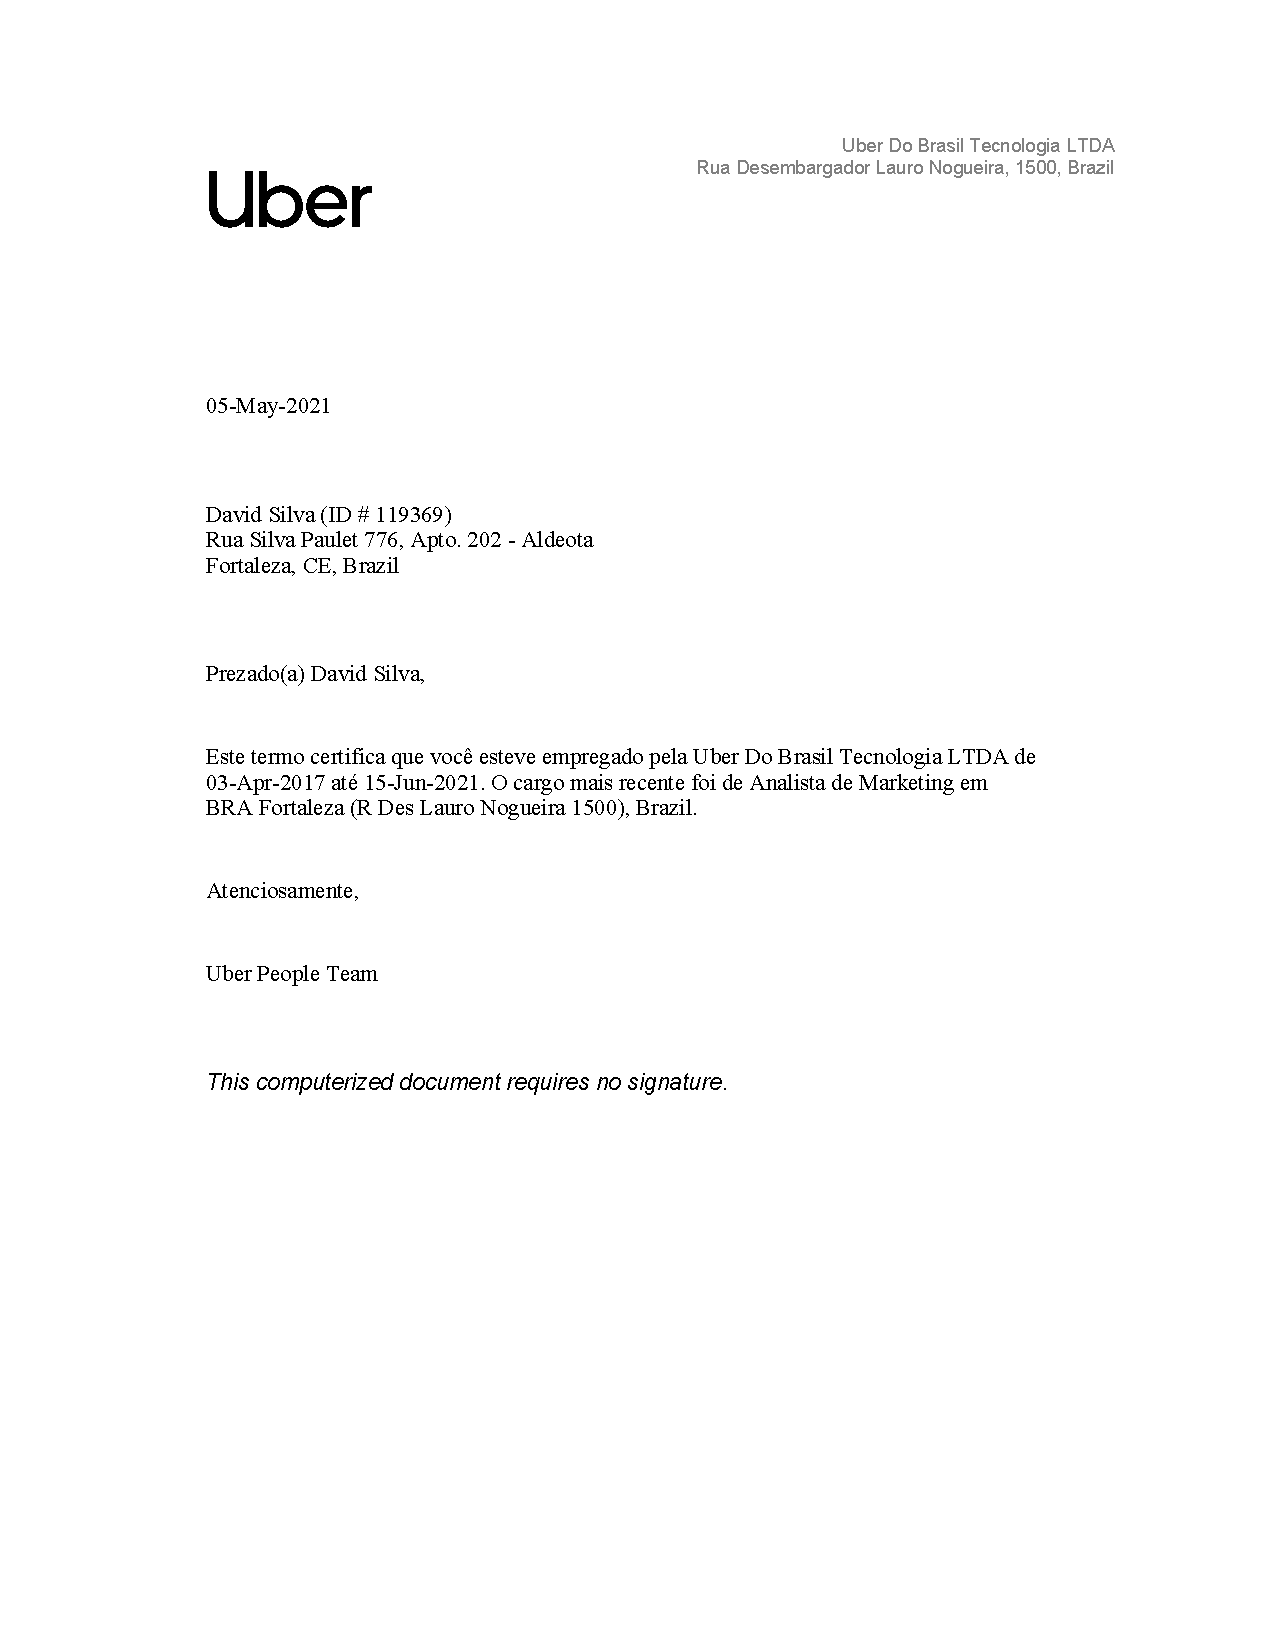
\includegraphics[scale=0.95]{Carta Uber.pdf}\\
\end{paracol}
%--------------------------------------------------------------------------------------

% use ONLY \newpage if you want to force a page break for
% ONLY the currentc column
%\newpage
%% Set the left/right column width ratio to 1:0.
%\columnratio{1.0}

\end{document}
